\documentclass[a4paper,13pt]{scrreprt}

\usepackage[francais]{babel}

\usepackage[utf8]{inputenc}
\usepackage[T1]{fontenc}
\usepackage{pifont}
%\usepackage{verdana}
\usepackage{ulem}


\usepackage{amsmath}
\usepackage{amssymb}
\usepackage{amsthm}
\usepackage{amscd}
\usepackage{mathabx}
\usepackage{hyperref}
\usepackage{setspace} 
\usepackage{multicol}
\onehalfspacing

\usepackage[abbrev,backrefs]{amsrefs}
\usepackage{eurosym}

\usepackage{graphicx}
\usepackage{array}

\usepackage{tikz,tkz-tab}
\usepackage{pgfplots}
\usepackage{tkz-fct}
\usetkzobj{all}

\usepackage[all]{xy}

\usepackage{geometry}
\geometry{hmargin=2.5cm,vmargin=2.5cm}
\pagestyle{myheadings}
\renewcommand{\chaptermark}[1]{\markboth{\textbf{\thechapter. #1}}{}}
\renewcommand{\sectionmark}[1]{\markright{\textbf{\thesection. #1}}}

\renewcommand{\familydefault}{\sfdefault}

\theoremstyle{plain}
\newtheorem{thé}[subsection]{Théorème}
\newtheorem*{thé*}{Théorème}
\newtheorem{pro}[subsection]{Proposition}
\newtheorem{cor}[subsection]{Corollaire}	
\newtheorem*{cor*}{Corollaire}
\newtheorem{lem}[subsection]{Lemme}		

\theoremstyle{definition}
\newtheorem{déf}[subsection]{Définition}
\newtheorem{exe}[subsection]{Exemple}
\newtheorem{con}[subsection]{Contre-exemple}
\newtheorem{rema}[subsection]{Remarque}	
\newtheorem*{rema*}{Remarque}	
\newtheorem*{nota}{Notation}
\newtheorem*{prob}{Problème}	
\newtheorem*{epcs}{Exercices pour cette section}
\newtheorem{exo}[subsection]{Exercice}

\newcommand{\nn}{\mathbb{N}}
\newcommand{\nno}{\mathbb{N}_{0}}
\newcommand{\zz}{\mathbb{Z}}
\newcommand{\qu}{\mathbb{Q}}
\newcommand{\rr}{\mathbb{R}}
\newcommand{\cc}{\mathbb{C}}
\newcommand{\imp}{\Rightarrow}

\DeclareMathOperator{\dom}{dom}
\DeclareMathOperator{\im}{im}

\begin{document}
	
\begin{titlepage}
	
	\newcommand{\HRule}{\rule{\linewidth}{0.5mm}} % Defines a new command for the horizontal lines, change thickness here
	
	\center % Center everything on the page
	
	%----------------------------------------------------------------------------------------
	%	HEADING SECTIONS
	%----------------------------------------------------------------------------------------
	
	\vspace{4cm}
	
	\textsc{\Large Cours de mahématiques de cinquième année \\ 4 périodes/semaine \\ Année 2018-2019}\\[0.5cm]
	\vspace{9.6cm}
	\textsc{\LARGE Rappels et compléments}\\[1cm] % Major heading such as course name
	\vspace{10cm}
	\textsc{\Large Lycée Martin V}\\[0.5cm] % Minor heading such as course title
	

	
\end{titlepage}
	

\tableofcontents

\chapter{Introduction et rappels sur les ensembles}

\section{Rappels... et compléments}

Ce premier chapitre du cours de mathématiques de cinquième année est dédié à toute une série de rappels des années précédentes, en particulier de la quatrième année. Néanmoins, ces rappels sont agrémentés de quelques nouveautés. Les thèmes abordés sont les équations et les inéquations, les polynômes, les droites et les paraboles et enfin les fonctions. \\
Ce premier chapitre est l'occasion de se remettre à niveau. Insistons sur ce point : à l'issue de ce chapitre, les notions mentionnées ci-dessus doivent être absolument maîtrisées. En effet, la matière du cours de mathématiques de cinquième année étant d'une complexité supérieure à tout ce qui a été fait dans les années antérieures, les notions abordées dans ce chapitre de rappels et qui sont utilisées systématiquement comme outils dans les chapitres suivants ne peuvent en aucun cas constituer un frein supplémentaire à la compréhension. \\
En fonction de la maîtrise que chacun a déjà des notions traitées, la charge de travail que demandera ce chapitre peut être quasi nulle ou plus grande que celles de tous les chapitres à venir. Malgré tout, il est impératif de fournir la charge de travail nécessaire pour avoir une bonne maîtrise de la matière abordée dans ce chapitre, de manière à réduire significativement la charge de travail requise pour les chapitres suivants.

\section{Rappels sur les ensembles}

Les mathématiques modernes sont généralement formulées dans le langage de la théorie des ensembles, un formalisme incroyablement puissant créé par Georg Cantor à la fin du dix-neuvième siècle. La révolution pour les mathématiques qu'a été cette théorie des ensembles ne peut malheureusement pas être exposée en détail dans le cadre d'un cours de mathématiques de secondaire, mais la richesse d'expressivité de cette théorie et la relative simplicité de ses versions les plus naïves justifient qu'elle soit utilisée dans notre cours. Rappelons donc quelques définitions de la théorie des ensembles naïve ainsi que quelques notations.

\newpage

\begin{déf}
	Un \emph{ensemble} est une collection d'objets, objets qui \emph{appartiennent} à cet ensemble et sont appelés ses \emph{éléments}. Deux ensembles sont égaux si et seulement si ils ont les mêmes éléments.
\end{déf}
\begin{nota}
	Les symboles $\{$ et $\}$ sont généralement utilisés pour noter un ensemble. Le symbole $\in$ désigne l'appartenance.
\end{nota}
\begin{exe}
	$\{1,13,\star\}$ est un ensemble qui contient trois éléments : $1$, $13$ et $\star$. \og $\star$ est un élément de $\{1,13,\star\}$ \fg{} se note $\star \in \{1,13,\star\}$. \\
	L'ensemble $\{1,13,\star\}$ est le même ensemble que $\{13,1,\star\}$, mais est différent de l'ensemble $\{1,13\}$.
\end{exe}
\begin{déf}
	Un ensemble $A$ est \emph{inclus} dans un ensemble $B$ si tous les éléments de $A$ appartiennent aussi à $B$.
\end{déf}
\begin{nota}
	\og L'ensemble $A$ est inclus dans l'ensemble $B$ \fg{} se note $A \subseteq B$.
\end{nota}
\begin{exe}
	L'ensemble $\{1,\star\}$ est inclus dans l'ensemble $\{1,13,\star\}$ : $\{1,\star\} \subseteq \{1,13,\star\}$. \\
	L'ensemble $\{1,13,\star\}$ n'est pas inclus dans l'ensemble $\{1,\star\}$ car $13 \in \{1,13,\star\}$ mais $13$ n'appartient pas à $\{1,\star\}$ : $13 \notin \{1,\star\}$.
\end{exe}
\begin{déf}
	\emph{L'union} de deux ensembles $A$ et $B$ est l'ensemble qui contient les éléments de $A$ et les éléments de $B$.
\end{déf}
\begin{nota}
	L'union de deux ensembles $A$ et $B$ se note $A\cup B$.
\end{nota}
\begin{exe}
	$\{1,13,\star\} \cup \{1,\star\} = \{1,13,\star\}$ et $\{1,13\} \cup \{1,\star\} = \{1,13,\star\}$.
\end{exe}
\begin{déf}
	\emph{L'intersection} de deux ensembles $A$ et $B$ est l'ensemble des éléments de $A \cup B$ qui appartiennent à $A$ et appartiennent à $B$.
\end{déf}
\begin{nota}
	L'intersection de deux ensembles $A$ et $B$ se note $A\cap B = \{x \in A \cup B ~|~x \in A$ et $x\in B\}$.
\end{nota}
\begin{exe}
	$\{1,13,\star\} \cap \{1,\star\} = \{1,\star\}$ et $\{1,13\} \cap \{1,\star\} = \{1\}$.
\end{exe}
\begin{déf}
	La \emph{différence} d'un ensemble $A$ par un ensemble $B$ est l'ensemble des éléments de $A$ qui n'appartiennent pas à $B$
\end{déf}
\begin{nota}
	La différence d'un ensemble $A$ par un ensemble $B$ se note $A \backslash B = \{x \in A  ~|~x\notin B\}$.
\end{nota}
\begin{exe}
	$\{1,13,\star\} \backslash \{1,\star\} = \{13\}$ et $\{1,13\} \cap \{\star\} = \{1,13\}$.
\end{exe}
\begin{déf}
	Le \emph{produit cartésien} de deux ensembles $A$ et $B$ est l'ensemble des couples $(a,b)$ où $a\in A$ et $b \in B$.
\end{déf}
\begin{nota}
	Le produit cartésien de deux ensembles $A$ et $B$ se note $A \times B$.
\end{nota}
\begin{exe}
	$\{1,13\} \times \{1,\star\} = \{(1,1),(1,\star),(13,1),(13,\star)\}$. On a par exemple $(1,\star) \in \{1,13\} \times \{1,\star\}$.
\end{exe}

Il existe des ensembles si importants en mathématiques qu'ils ont leur propre symbole. Le premier est l'ensemble vide :

\begin{déf}
	\emph{L'ensemble vide}, noté $\emptyset$, est l'ensemble qui ne contient aucun élément.
\end{déf}

Les ensembles les plus connus sont les ensembles de nombres. Rappelons ceux-ci, du plus simple au plus complexe.

\begin{déf}
	\emph{L'ensemble des nombres naturels}, noté $\nn$, est l'ensemble $\{0,1,2,3...\}$.
\end{déf}
\begin{rema}
	La principale utilité des nombres naturels est de permettre de compter et dénombrer. Ils permettent également de calculer dans une moindre mesure : on peut toujours additionner ou multiplier deux nombres naturels, mais on ne peut pas toujours les soustraire entre eux ($4-7=-3$ n'est pas un nombre naturel) ou les diviser entre eux ($4/3$ n'est pas un nombre naturel).
\end{rema}

\begin{déf}
	\emph{L'ensemble des nombres entiers}, noté $\zz$, est l'ensemble $\{...,-3,-2,-1,0,1,2,3...\}$.
\end{déf}
\begin{rema}
	La principale utilité des nombres entiers est de calculer avec des valeurs entières : on peut toujours additionner ou multiplier deux nombres entiers et on peut aussi toujours les soustraire entre eux ! Mais on ne peut pas toujours les diviser entre eux ($-4/3$ n'est pas un nombre entier).
\end{rema}

\begin{déf}
	\emph{L'ensemble des nombres rationnels}, noté $\qu$, est l'ensemble des fractions de nombres entiers : $\frac{a}{b}$ avec $a,b \in \zz$ et $b \neq 0$ (on ne divise pas par $0$).
\end{déf}
\begin{rema}
	La principale utilité des nombres rationnels est de calculer avec des valeurs fractionnaires : on peut toujours additionner, multiplier, soustraire et diviser (à condition que le deuxième soit non nul, bien entendu) deux nombres rationnels.
\end{rema}

\begin{déf}
	\emph{L'ensemble des nombres réels}, noté $\rr$, est l'ensemble des nombres qui peuvent être représentés par un nombre entier et une suite finie ou infinie de décimales.
\end{déf}
\begin{rema}
	On considère généralement que ce sont tous les nombres qu'on peut retrouver dans la réalité physique et une interprétation géométrique classique est celle des points d'une droite (infinie) : à chaque point de la droite correspond un nombre réel.
\end{rema}
\begin{rema}
	En plus de tous les nombres rationnels, $\rr$ contient des nombres comme $\sqrt{2}$ ou $\pi$, qui sont évidemment très utiles.
\end{rema}
Notons qu'il y a donc une hiérarchie parmi les ensembles de nombres :
$$\nn \subseteq \zz \subseteq \qu \subseteq \rr$$
Pour terminer, rappelons quelques notations ainsi que la définition d'intervalle (réel) :
\begin{nota}
	~~\\
	${\rr}_{0} = \rr \backslash \{0\}$ \\
	${\rr}^{+} = \{x \in \rr~|~x \ge 0\}$ \\
	${\rr}^{-} = \{x \in \rr~|~x \le 0\}$ \\
	${\rr}^{2} = \rr \times \rr$ \\
	${\rr}^{3} = \rr \times \rr \times \rr$
\end{nota}
\begin{déf}
	Un \emph{intervalle} (réel) est un sous-ensemble de $\rr$, $I \subseteq \rr$, tel que si on a deux nombres réels $x,y \in \rr$ avec $x < y$, $x \in I$ et $y \in I$, alors tout nombre réel $z \in \rr$ qui est compris entre $x$ et $y$ (c'est-à-dire tel que $x\le z \le y$) est nécessairement dans $I$ (c'est-à-dire que $z \in I$).
\end{déf}
Il n'existe pas un très grand nombre de formes possibles pour les intervalles réels. En dehors de $\rr$ et $\emptyset$, tous les intervalles réels sont d'une des formes suivantes :
\begin{nota}
	Soient deux nombres réels $a$ et $b$. \\
	\begin{itemize}
		\item [$\bullet$] $[a,b] = \{x \in \rr~|~a \le x \le b\}$
		\item [$\bullet$] $[a,b[ = \{x \in \rr~|~a \le x < b\}$
		\item [$\bullet$] $]a,b] = \{x \in \rr~|~a < x \le b\}$
		\item [$\bullet$] $]a,b] = \{x \in \rr~|~a < x < b\}$
		\item [$\bullet$] $[a,\infty[ = \{x \in \rr~|~a \le x\}$
		\item [$\bullet$] $]a,\infty[ = \{x \in \rr~|~a < x\}$
		\item [$\bullet$] $]-\infty,b] = \{x \in \rr~|~x \le b\}$
		\item [$\bullet$] $]-\infty,b[ = \{x \in \rr~|~x < b\}$
	\end{itemize}
\end{nota}
~\\
Pour approfondir et s'entraîner avec quelques exercices, je vous renvoie vers le site \href{https://www.auto-math.be/public/0/module/2}{Auto-Math}.
\chapter{Les équations et les inéquations}

\section{Les équations} \label{sectionequation}

Dans de nombreux cas, la résolution d'un problème formalisé à l'aide des mathématiques consiste en la résolution d'une équation. Afin de pouvoir se concentrer sur les mathématiques elles-mêmes et les idées belles et ingénieuses qu'on met en place afin de résoudre de nouveaux problèmes, il faut être à même de résoudre des équations simples avec aisance.

\begin{déf}
	Une \emph{équation} est une égalité qui n'est vérifiée que pour certaines valeurs données aux variables qu'elle contient. Ces variables sont les \emph{inconnues} de l'équation et les valeurs qui vérifient l'équation sont appelées les \emph{solutions} de l'équation.
\end{déf}

\begin{exe}
	$2x+7=x-1$ est une équation à une inconnue : $x$. De plus, $-8$ est une solution de cette équation : si on remplace la variable $x$ par $-8$, on obtient une égalité : $2(-8)+7=-9=-8-1$.
\end{exe}


Lorsqu'on demande de résoudre une équation, il faut normalement préciser ce que peuvent contenir les variables de l'équation, autrement dit dans quel ensemble on recherche les solutions de l'équation. Les solutions d'une équation dépendent du type de solution qu'on recherche. Par exemple :
\begin{exe}
	Avec l'équation $x^2=4$, le fait de savoir si on cherche tous les nombres entiers $x$ tels que $x^2=4$ ou tous les nombres entiers \textbf{positifs} a de l'importance. Dans le premier cas, l'équation a deux solutions : $2$ et $-2$. Dans le second cas, l'équation a seulement une solution : $2$ (parce que $-2$ n'est pas un nombre entier positif).
\end{exe}
Notons qu'une équation peut ne pas avoir de solution. Par exemple :
\begin{exe}
	Si on cherche les nombres réels $x$ qui vérifient l'équation $x^2=-1$, il n'y a pas de solution. En effet, tous les carrés de nombres réels sont des nombres positifs, mais $-1$ est un nombre strictement négatif.
\end{exe}

\newpage

Pour résoudre des équations, on utilise les propriétés de l'identité et des opérations. \\ Pour des nombres réels $a,b,c,d$ quelconques, on a :

\begin{enumerate}
	\item $a=a$~~~~~~(Tout nombre est égal à lui-même !)
	\item Si $a=b$, alors $b=a$.
	\item Si $a=b$ et $b=c$, alors $a=c$.
	\item Si $a=b$, alors $a+c=b+c$.
	\item Si $a=b$, alors $a-c=b-c$.
	\item Si $a=b$, alors $a.c=b.c$.
	\item Si $a=b$, \textbf{à la condition que} $c \neq 0$ (on ne divise pas par $0$), alors $\frac{a}{c}=\frac{b}{c}$.
	\item Si $a=b$ et $c=d$, alors $a+c=b+d$.
\end{enumerate}
Ces règles de calcul vous sont connues depuis longtemps, ne fût-ce qu'intuitivement. En plus de ces règles de calcul élémentaires, on peut ajouter les propriétés de l'addition et de la multiplication :
\begin{enumerate}
	\item $(a+b)+c=a+(b+c)$~~~~~~(associativité de l'addition)
	\item $a+b=b+a$~~~~~~(commutativité de l'addition)
	\item $a.(b.c)=(a.b).c$~~~~~~(associativité de la multiplication)
	\item $a.b=b.a$~~~~~~(commutativité de la multiplication)
	\item $a.(b+c)=a.b+a.c$~~~~~~(distributivité)
\end{enumerate}

\begin{rema}
	Lorsqu'une équation fait intervenir un polynôme de degré supérieur ou égal à deux (voir section \ref{sectionpoly} pour un rappel sur les polynômes), il est souvent nécessaire de factoriser un polynôme pour résoudre une équation, autrement dit le réécrire sous la forme d'une produit de polynômes de degrés plus petits. Rappelons les formules suivantes, souvent très utiles. \\
	Pour des nombres réels $a,b$ quelconques, on a:
	\begin{enumerate}
		\item $(a+b)^2=(a+b)(a+b)=a.(a+b)+b.(a+b)=a^2+ab+ba+b^2=a^2+2ab+b^2$
		\item $(a+b)(a-b)=a(a-b)+b(a-b)=a^2-ab+ba-b^2=a^2-b^2$
		\item $(a+b)^3=(a^2+2ab+b^2)(a+b)=a^2.(a+b)+2ab.(a+b)+b^2.(a+b)=a^3+a^2 b + 2a^2 b + 2a b^2 + ab^2 + b^3 = a^3 + 3a^2b + 3ab^2 + b^3$
		\item $(a-b)(a^2+ab+b^2)=a^3 + a^2 b + ab + a b^2 - a^2 b - ab^2 - b^3 = a^3 - b^3$
	\end{enumerate}
\end{rema}

\newpage

\begin{rema}
	Une autre démarche nécessaire pour résoudre certaines équations faisant intervenir des fractions est la mise au même dénominateur. Rappelons donc que pour quatre nombres réels $a,b,c,d$ tels que $b \ne 0$ et $d \ne 0$, on a :$$\frac{a}{b}+\frac{c}{d}=\frac{ad}{bd}+\frac{cb}{db}=\frac{ad+bc}{bd}$$
\end{rema}

\begin{epcs}
	~~\\
	Exercices faciles : \ref{exoei1}, \ref{exoei8}, \ref{exoei9}, \ref{exoei10}, \ref{exoei11}, \ref{exoei12}.\\
	Exercices moyens : \ref{exoei2}.\\
	Exercices difficiles : \ref{exoei3}, \ref{exoei4}.
\end{epcs}

\section{Les inéquations} \label{sectioninequation}

Dans certains cas, la résolution d'un problème revient à la résolution d'une inéquation plutôt que d'une équation, par exemple lorsqu'on recherche une borne maximale pour une variable.

\begin{déf}
	Une \emph{inéquation} est une inégalité qui n'est vérifiée que pour certaines valeurs données aux variables qu'elle contient. Ces variables sont les \emph{inconnues} de l'inéquation et les valeurs qui vérifient l'inéquation sont appelées les \emph{solutions} de l'inéquation.
\end{déf}
\begin{exe}
	$j+1 \ge -6$ est une inéquationà une inconnue : $j$. De plus, $0$ est une solution de cette équation : si on remplace la variable $j$ par $0$, l'inégalité est vérifiée : $0+1 \ge -6$.
\end{exe}
Comme pour les équations, lorsqu'on demande de résoudre une inéquation, il faut normalement préciser ce que peuvent contenir les variables de l'inéquation, autrement dit dans quel ensemble on recherche les solutions de l'inéquation. Les solutions d'une inéquation dépendent du type de solution qu'on recherche. Par exemple :
\begin{exe}
	Avec l'inéquation $2x \le 7$, le fait de savoir si on cherche tous les nombres réels $x$ tels que $2x \le 7$ ou tous les nombres entiers positifs $x$ tels que $2x \le 7$ a de l'importance. Dans le premier cas, l'inéquation a une infinité de solutions : tous les nombres réels plus petits que $\frac{7}{2}$. Dans le second cas, l'inéquation a seulement quatre solutions : $0,1,2,3$.
\end{exe}
Notons qu'une inéquation peut ne pas avoir de solution. Par exemple :
\begin{exe}
	Si on cherche les nombres réels $x$ qui vérifient l'équation $x^2 \le -1$, il n'y a pas de solutions. En effet, tous les carrés de nombres réels sont des nombres positifs, mais $-1$ est un nombre strictement négatif.
\end{exe}

\newpage

Pour résoudre des inéquations, on utilise les propriétés de l'inégalité et des opérations. \\ Pour des nombres réels $a,b,c,d$ quelconques, on a :

\begin{enumerate}
	\item Tout nombre est plus grand ou égal à lui-même : $a \ge a$.
	\item Si $a \ge b$ et $b \ge c$, alors $a \ge c$.
	\item Si $a \ge b$, alors $a+c \ge b+c$.
	\item Si $a \ge b$, alors $a-c \ge b-c$.
	\item Si $a \ge b$, \textbf{à la condition que} $c \ge 0$, alors $a.c \ge b.c$.
	\item Si $a \ge b$, \textbf{à la condition que} $c < 0$, alors $a.c \le b.c$. (Si $c<0$, le sens de l'inégalité est renversé.)
	\item Si $a \ge b$, \textbf{à la condition que} $c > 0$, alors $\frac{a}{c} \ge \frac{b}{c}$.
	\item Si $a \ge b$, \textbf{à la condition que} $c < 0$, alors $\frac{a}{c} \le \frac{b}{c}$. (Si $c<0$, le sens de l'inégalité est renversé.)
	\item Si $a \ge b$ et $c \ge d$, alors $a+c \ge b+d$.
	\item Si $a \ge b$ et $c \le d$, alors $a-c \ge b-d$.
	\item Si $b \ge a$ et $a > 0$, alors $\frac{1}{a} \ge \frac{1}{b}$.
\end{enumerate}
\begin{rema}
	Attention aux propriétés $6$, $8$, $10$ et $11$ : ne pas les respecter scrupuleusement est source de nombreuses erreurs !
\end{rema}

\begin{epcs}
	~~\\
	Exercices faciles : \ref{exoei5}, \ref{exoei5a}, \ref{exoei5b}, \ref{exoei5c}.\\
	Exercices difficiles : \ref{exoei6}, \ref{exoei7}.
\end{epcs}

\chapter{Les polynômes, les droites et les paraboles}

\section{Définitions} \label{sectionpoly}
	
Les polynômes sont des objets mathématiques qui apparaissent très souvent dans les équations et dans les inéquations que l'on doit résoudre pour trouver la solution à un problème.

\begin{déf}
	Un \emph{polynôme} en la variable $x$ est une somme dont les termes sont des produits de puissances entières positives ou nulles de la variable $x$ par des nombres réels. Les facteurs réels de ces produits sont appelés les \emph{coefficients} du polynôme. Le \emph{degré} du polynôme est le degré du terme de plus haute puissance de la variable dont le coefficient est non nul. Le \emph{terme indépendant} du polynôme est le terme de puissance nulle.
\end{déf}

\begin{exe}
	$7x^7 + x^2 +\frac{1}{4}$, $\pi x^{1000} -6$, $2x$ et $3$ sont quatre polynômes, respectivement de degrés $7$, $1000$, $1$ et $0$ et de termes indépendants $\frac{1}{4}$, $-6$, $0$ et $3$.
\end{exe}
\begin{con}
	$x^2 + 2\sqrt{x}$ n'est pas un polynôme. En effet, bien que $\sqrt{x}$ puisse être réécrit à l'aide d'une puissance ($\sqrt{x}=x^{\frac{1}{2}}$), cette puissance ($\frac{1}{2}$) n'est pas un nombre entier positif.
\end{con}
\begin{rema}
	Deux polynômes sont égaux si et seulement si les termes de même puissance ont les mêmes coefficients.
\end{rema}
Bien souvent, pour résoudre un problème, il faut trouver la racine d'un polynôme :
\begin{déf}
	Un nombre réel $a$ est une \emph{racine} d'un polynôme $c_n x^n + c_{n-1} x^{n-1} + ... + c_2 x^2 + c_1 x^1 + c_0$ (où $c_n , c_{n-1} , ... , c_2 , c_1 , c_0$ sont les coefficients du polynômes, autrement dit des nombres réels) si lorsqu'on remplace la variable $x$ par $a$ (lorsqu'on \emph{évalue} le polynôme en $a$), le résultat est égal à $0$. Autrement dit, si $c_n a^n + c_{n-1} a^{n-1} + ... + c_2 a^2 + c_1 a + c_0 = 0$.
\end{déf}
\begin{exe}
	Le nombre $-1$ est racine du polynôme $x^2-3x-4$. En effet : $(-1)^2 - 3(-1) - 4 = 1 + 3 - 4 = 0$.
\end{exe}
\begin{con}
	Le nombre $\pi$ n'est pas une racine du polynôme $x^{17}-x+1$. En effet : ${\pi}^{17} - \pi + 5 \neq 0$.
\end{con}

\begin{rema}
	Il est possible d'additionner, de multiplier et même de diviser des polynômes :
	\begin{itemize}
		\item [$\bullet$] La \emph{somme} de deux polynômes est le polynôme obtenu en additionnant entre eux les termes de même puissance. \\
		Par exemple : la somme de $4x^4 - x^2 - \frac{3}{4}x +1$ et de $3x^2 - \pi$ est $4x^4 + (-x^2 + 3x^2) - \frac{3}{4}x + (1 - \pi) = 4x^4 + 2x^) - \frac{3}{4}x + 1 - \pi$. \\
		
		\item [$\bullet$] Le \emph{produit} de deux polynômes est le polynôme obtenu en multipliant chaque terme de l'un par chaque terme de l'autre. \\
		Par exemple : le produit de $ - 4x^2 - 3x +\frac{1}{2}$ et de $\sqrt{17}x + 12$ est $- (4x^2 - 3x +\frac{1}{2}).\sqrt{17}x + (4x^2 - 3x +\frac{1}{2}). 12 = (4\sqrt{17}x^3 - 3\sqrt{17}x^2 +\frac{\sqrt{17}}{2}x) + (48x^2 - 36x + 6) = 4\sqrt{17}x^3 + (- 3\sqrt{17}x^2 + 48x^2) + (\frac{\sqrt{17}}{2}x+36x)+6 = 4\sqrt{17}x^3 + (- 3\sqrt{17} + 48)x^2 + (\frac{\sqrt{17}}{2}+36)x + 6$. \\
		\item [$\bullet$] La \emph{division} d'un polynôme par un autre polynôme est un peu plus complexe. Elle n'est possible que si le degré du polynôme divisé, le \emph{dividende}, est plus grand ou égal au degré du polynôme qui divise, le \emph{diviseur}\footnote{Sinon, c'est un peu comme essayer de diviser dans les naturels un petit nombre par un grand nombre : on peut par exemple effectuer la division entière de $1000$ par $10$, mais il n'y a aucune chance qu'on puisse effectuer la division entière de $10$ par $1000$. De la même manière, on peut par exemple diviser $x^7$ par $x^3$, mais aucune chance qu'on puisse diviser $x^3$ par $x^7$.}. Le but de la division d'un polynôme $P(x)$ par un polynôme $D(x)$ est d'obtenir deux polynômes, $Q(x)$ (le \emph{quotient}) et $R(x)$ (le \emph{reste}), tels que :
		\begin{itemize}
			\item [$\bullet$] $P(x) = Q(x).D(x) + R(x)$
			\item [$\bullet$] Le degré de $R(x)$ est strictement plus petit que celui de $D(x)$.
			\item [$\bullet$] Le degré de $Q(x)$ est égal au degré de $D(x)$ moins le degré de $Q(x)$\footnote{Si le degré de $D(x)$ était plus grand que celui de $P(x)$, le degré de $Q(x)$ devrait être... négatif. Ce qui n'a pas de sens : le degré de $D(x)$ doit donc être plus grand que celui de $P(x)$.}.
		\end{itemize}
		Il y a deux méthodes pour calculer la division d'un polynôme par un autre polynôme. La première, la méthode de la division euclidienne, fonctionne toujours. La seconde, la méthode de Horner, ne fonctionne que lorsque le diviseur est un polynôme de degré $1$. Nous ne présentons ici que la première, volontairement, mais un rappel sur la méthode de Horner peut être trouvé sur cette page : \url{https://www.auto-math.be/public/0/module/10/theorie/37}.
\newpage
		\begin{exe}
			La division euclidienne pour les polynômes fonctionne de façon similaire à la division euclidienne pour les nombres entiers à l'aide d'un tableau du type :
			\begin{equation*}
			\renewcommand{\arraystretch}{1.2}
			\renewcommand{\arraycolsep}{2pt}
			\begin{array}{r|r}
			P(x) & D(x)  \\
			\cline{2-2}
			\vdots~~~~ & Q(x)\\
			\cline{1-1}
			R(x) &   
			\end{array}
			\end{equation*}
			Le processus se termine quand le degré du polynôme $R(x)$ est strictement plus petit que le degré du polynôme $D(x)$. \\
			~~\\
			Procédons étape par étape sur un exemple : divisons $P(x)=2x^3+x^2-1$ par $D(x)=3x^2-1$. On commence avec le tableau suivant :
			\begin{equation*}
			\renewcommand{\arraystretch}{1.2}
			\renewcommand{\arraycolsep}{2pt}
			\begin{array}{rrrr|rr}
			2x^3&+x^2 &   &-1&3x^2  &-1  \\
			\cline{5-6}
			   &    &   &  &   &   \\
			&  & &  &   &  \\
			&  &   &   &   &  \\
			&     &   &   &   &  
			\end{array}
			\end{equation*}
			On divise le premier terme (celui de plus haut degré) du dividende par celui du diviseur : $2x^3$ divisé par $3x^2$ donne $\frac{2}{3}x$. On inscrit ce résultat à la place du quotient :
			\begin{equation*}
			\renewcommand{\arraystretch}{1.2}
			\renewcommand{\arraycolsep}{2pt}
			\begin{array}{rrrr|rr}
			2x^3&+x^2 &   &-1&3x^2  &-1  \\
			\cline{5-6}
			&    &   &  &\frac{2}{3}x&   \\
			&  & &  &   &  \\
			&  &   &   &   &  \\
			&     &   &   &   &  
			\end{array}
			\end{equation*}
			On multiplie ensuite ce début de quotient par le diviseur, $(\frac{2}{3}x).(2x^2 -1) = 2x^3 - \frac{2}{3}x$, et on soustrait le résultat du dividende :
			\begin{equation*}
			\renewcommand{\arraystretch}{1.2}
			\renewcommand{\arraycolsep}{2pt}
			\begin{array}{rrrr|rr}
			2x^3&+x^2 &   &-1&3x^2  &-1  \\
			\cline{5-6}
			-2x^3&    &+\frac{2}{3}x&  &\frac{2}{3}x&   \\
			\cline{1-3}
			&x^2 &+\frac{2}{3}x&  &   &  
			\end{array}
			\end{equation*}
			~~\\
			On recommence jusqu'à avoir terminé :
			\begin{equation*}
			\renewcommand{\arraystretch}{1.2}
			\renewcommand{\arraycolsep}{2pt}
			\begin{array}{rrrr|rr}
			2x^3&+x^2 &   &-1&3x^2  &-1  \\
			\cline{5-6}
			-2x^3&    &+\frac{2}{3}x&  &\frac{2}{3}x&+\frac{1}{3}\\
			\cline{1-3}
			&x^2 &+\frac{2}{3}x&  &   &  \\
			&-x^2&   &-\frac{1}{3}&   &  \\
			\cline{2-4}
			&     &\frac{2}{3}x&-\frac{4}{3}&   &  
			\end{array}
			\end{equation*}
			À ce stade, le degré de du polynôme $\frac{2}{3}x-\frac{4}{3}$ (qui est égal à $1$) est strictement plus petit que le degré du polynôme $3x^2-1$ (qui est égal à $2$). Le processus est donc terminé, et on a :
			$$2x^3+x^2-1 = \left(\frac{2}{3}x+\frac{1}{3}\right)\left(3x^2-1\right) + \left(\frac{2}{3}x-\frac{4}{3}\right)$$
		\end{exe}
	\end{itemize}
\end{rema}
Terminons par une proposition très simple à démontrer et son corollaire extrêmement utile.
\begin{pro}
	Soit $a$ un nombre réel. Soit $P(x)=c_n x^n + c_{n-1} x^{n-1} + ... + c_2 x^2 + c_1 x^1 + c_0$ un polynôme de degré égal ou supérieur à $1$. \\
	Le reste de la division du polynôme $P(x)$ par $(x-a)$ est égal à $P(a) = c_n a^n + c_{n-1} a^{n-1} + ... + c_2 a^2 + c_1 a^1 + c_0$.
\end{pro}
\begin{proof} \label{diveuc}
	La division euclidienne de $P(x)$ par $(x-a)$ nous donne deux polynômes $Q(x)$ et $R(x)$ tels que :
	$$P(x) = Q(x).(x-a)+R(x)$$
	où le degré de $R(x)$ est strictement plus petit que celui de $(x-a)$ (qui est égal à $1$) et donc égal à $0$. Autrement dit, $R(x)$ est un polynôme constant : quel que soit $x$, $R(x)=k$ pour un certain nombre réel $k$. Il nous reste à montrer que $P(a)=k$. Pour ce faire, il suffit de remplacer $x$ par $a$ dans l'équation ci-dessus :
	$$P(a) = Q(a).(a-a)+R(a)= Q(a).0 + k = k$$
\end{proof}
\begin{cor}
	Soit $a$ un nombre réel. Soit $P(x)=c_n x^n + c_{n-1} x^{n-1} + ... + c_2 x^2 + c_1 x^1 + c_0$ un polynôme de degré égal ou supérieur à $1$. \\
	$P(x)$ est divisible par $(x-a)$ sans reste si et seulement si $a$ est une racine de $P(x)$.
\end{cor}
\begin{proof}
	Par la proposition \ref{diveuc}, le reste de la division de $P(x)$ par $(x-a)$ est égal à $P(a)$. Ce reste est donc nul si et seulement si $P(a)=0$, autrement dit si $a$ est une racine de $P(x)$.
\end{proof}
\begin{epcs}
	~~\\
	Exercices faciles : \ref{exop1},\ref{exop2}, \ref{exop2a}, \ref{exop2b}.\\
	Exercices moyens :  \ref{exop2c}.\\
	Exercices difficiles : \ref{exop3}.
\end{epcs}

\section{Les droites}

Supposons nous être donné un repère orthonormé du plan ${\rr}^2$ :
\begin{center}
\begin{tikzpicture}
\begin{axis}[ xmin=-5, xmax=5, ymin=-5, ymax=5, extra x ticks={-4,-3,-2,-1,0,1,2,3,4}, extra y ticks={-4,-3,-2,-1,0,1,2,3,4}, extra tick style={grid=major}, ]
\addplot[color=black] coordinates { (0,-5) (0,-4) (0,-3) (0,-2) (0,-1) (0,0) (0,1) (0,2) (0,3) (0,4) (0,5) };
\addplot[color=black] coordinates { (-5,0) (-4,0) (-3,0) (-2,0) (-1,0) (0,0) (1,0) (2,0) (3,0) (4,0) (5,0) };
\end{axis}
\end{tikzpicture}
\end{center}

Dans ce contexte, l'objet géométrique que sont les droites peuvent être reliés aux polynômes de degré 1 :
\begin{déf} \label{défdroite}
	Une \emph{droite} (non-verticale) est un ensemble de points $(x,y)$ du plan ${\rr}^2$ qui vérifie une équation du type $y = ax + b$ où $a$ et $b$ sont des nombres réels. L'équation $y = ax + b$ est appelée \emph{l'équation cartésienne} de la droite, le nombre $a$ est la \emph{pente} de la droite et le nombre $b$ est \emph{l'ordonnée à l'origine} de la droite.
\end{déf}
\begin{exe}
	L'ensemble $\{(x,y) \in {\rr}^2 ~|~ y = \frac{1}{2}x -1\}$, autrement dit l'ensemble des points $(x,y)$ du plan ${\rr}^2$ tels que l'équation $y=\frac{1}{2}x -1$ est vérifiée, est une droite de pente $\frac{1}{2}$ et d'ordonnée à l'origine $-1$ :
\begin{center}
	\begin{tikzpicture}
	\begin{axis}[ xmin=-5, xmax=5, ymin=-5, ymax=5, extra x ticks={-4,-3,-2,-1,0,1,2,3,4}, extra y ticks={-4,-3,-2,-1,0,1,2,3,4}, extra tick style={grid=major}, ]
	\addplot[color=black] coordinates { (0,-5) (0,-4) (0,-3) (0,-2) (0,-1) (0,0) (0,1) (0,2) (0,3) (0,4) (0,5) };
	\addplot[color=black] coordinates { (-5,0) (-4,0) (-3,0) (-2,0) (-1,0) (0,0) (1,0) (2,0) (3,0) (4,0) (5,0) };
	\addplot[color=blue] coordinates { (-5,-3.5) (-4,-3) (-3,-2.5) (-2,-2) (-1,-1.5) (0,-1) (1,-0.5) (2,0) (3,0.5) (4,1) (5,1.5) };
	\end{axis}
	\end{tikzpicture}
\end{center}
\end{exe}
\begin{déf}
	~~\\
	Deux droites sont \emph{parallèles} si et seulement si elles ont la mêmes pente. \\
	Deux droites sont \emph{sécantes} si et seulement si elles ont des pentes différentes.
\end{déf}
\begin{exe}
	Les deux droites d'équations cartésiennes $y= 2x -1$ et $y=2x-2$ sont parallèles :
	\begin{center}
		\begin{tikzpicture}
		\begin{axis}[ xmin=-5, xmax=5, ymin=-5, ymax=5, extra x ticks={-4,-3,-2,-1,0,1,2,3,4}, extra y ticks={-4,-3,-2,-1,0,1,2,3,4}, extra tick style={grid=major}, ]
		\addplot[color=black] coordinates { (0,-5) (0,-4) (0,-3) (0,-2) (0,-1) (0,0) (0,1) (0,2) (0,3) (0,4) (0,5) };
		\addplot[color=black] coordinates { (-5,0) (-4,0) (-3,0) (-2,0) (-1,0) (0,0) (1,0) (2,0) (3,0) (4,0) (5,0) };
		\addplot[color=blue] coordinates { (-2,-5) (-1,-3) (0,-1) (1,1) (2,3) (3,5) };
		\addplot[color=red] coordinates { (-1.5 ,-5) (-1,-4) (0,-2) (1,0) (2,2) (3,4) (3.5,5)};
		\end{axis}
		\end{tikzpicture}
	\end{center}
	~~\\
	Les deux droites d'équations cartésiennes $y= 2x -1$ et $y=-x+1$ sont sécantes :
		\begin{center}
			\begin{tikzpicture}
			\begin{axis}[ xmin=-5, xmax=5, ymin=-5, ymax=5, extra x ticks={-4,-3,-2,-1,0,1,2,3,4}, extra y ticks={-4,-3,-2,-1,0,1,2,3,4}, extra tick style={grid=major}, ]
			\addplot[color=black] coordinates { (0,-5) (0,-4) (0,-3) (0,-2) (0,-1) (0,0) (0,1) (0,2) (0,3) (0,4) (0,5) };
			\addplot[color=black] coordinates { (-5,0) (-4,0) (-3,0) (-2,0) (-1,0) (0,0) (1,0) (2,0) (3,0) (4,0) (5,0) };
			\addplot[color=blue] coordinates { (-2,-5) (-1,-3) (0,-1) (1,1) (2,3) (3,5) };
			\addplot[color=red] coordinates { (-4,5) (-3,4) (-2,3) (-1,2) (0,1) (1,0) (2,-1) (3,-2) (4,-3) (5,-4) };
			\end{axis}
			\end{tikzpicture}
		\end{center}
\end{exe}
\begin{déf}
	~~\\
	Deux droites non-horizontales de pentes $a_1$ et $a_2$ sont perpendiculaires si et seulement si $a_1 = \frac{-1}{a_2}$.
\end{déf}
\begin{exe}
	Les deux droites d'équations cartésienne $y= 2x -1$ et $y=\frac{-1}{2}x+3$ sont perpendiculaires :
	\begin{center}
		\begin{tikzpicture}
		\begin{axis}[ xmin=-5, xmax=5, ymin=-5, ymax=5, extra x ticks={-4,-3,-2,-1,0,1,2,3,4}, extra y ticks={-4,-3,-2,-1,0,1,2,3,4}, extra tick style={grid=major}, ]
		\addplot[color=black] coordinates { (0,-5) (0,-4) (0,-3) (0,-2) (0,-1) (0,0) (0,1) (0,2) (0,3) (0,4) (0,5) };
		\addplot[color=black] coordinates { (-5,0) (-4,0) (-3,0) (-2,0) (-1,0) (0,0) (1,0) (2,0) (3,0) (4,0) (5,0) };
		\addplot[color=blue] coordinates { (-2,-5) (-1,-3) (0,-1) (1,1) (2,3) (3,5) };
		\addplot[color=red] coordinates { (-5,0.5) (-4,0) (-3,-0.5) (-2,-1) (-1,-1.5) (0,-2) (1,-2.5) (2,-3) (3,-3.5) (4,-4) (5,-4.5) };
		\end{axis}
		\end{tikzpicture}
	\end{center}
\end{exe}

\begin{epcs}
	~~\\
	Exercices faciles : \ref{exop4}.\\
	Exercices moyens : \ref{exop5}.\\
	Exercices difficiles : \ref{exop6}, \ref{exop7}, \ref{exop8}.
\end{epcs}

\section{Les paraboles}

Si les polynômes de degré 1 peuvent être reliés aux droites, les polynômes de degré 2 peuvent être reliés aux paraboles.

\begin{déf}
	Une \emph{parabole} est un ensemble de points $(x,y)$ du plan ${\rr}^2$ qui vérifie une équation du type $y = ax^2 + bx + c$ où $a$ est un nombre réel non-nul et $b,c$ sont des nombres réels quelconques. L'équation $y = ax^2 + bx + c$ est appelée \emph{l'équation cartésienne} de la parabole.
\end{déf}
\newpage
\begin{exe}
	L'ensemble $\{(x,y) \in {\rr}^2 ~|~ y = -2x^2 + 3x -1\}$, autrement dit l'ensemble des points $(x,y)$ du plan ${\rr}^2$ tels que l'équation $y = -2x^2 + 3x -1$ est vérifiée, est une parabole :
	\begin{center}
		\begin{tikzpicture}
		\begin{axis}[ xmin=-5, xmax=5, ymin=-5, ymax=5, extra x ticks={-4,-3,-2,-1,0,1,2,3,4}, extra y ticks={-4,-3,-2,-1,0,1,2,3,4}, extra tick style={grid=major}, ]
		\addplot[color=black] coordinates { (0,-5) (0,-4) (0,-3) (0,-2) (0,-1) (0,0) (0,1) (0,2) (0,3) (0,4) (0,5) };
		\addplot[color=black] coordinates { (-5,0) (-4,0) (-3,0) (-2,0) (-1,0) (0,0) (1,0) (2,0) (3,0) (4,0) (5,0) };
		\addplot[color=blue] coordinates { (-1,-6) (-0.75,-4.375) (-0.5,-3) (-0.25,-1.875) (0,-1) (0.125,-0.65625) (0.25,-0.375) (0.375,-0.15625) (0.5,0) (0.6,0.08) (0.7,0.12) (0.75,0.125) (0.8,0.12) (0.9,0.08) (1,0) (1.125,-0.15625) (1.25,-0.375) (1.375,-0.65625) (1.5,-1) (1.75,-1.875) (2,-3) (2.25,-4.375) (2.5,-6) };
		\end{axis}
		\end{tikzpicture}
	\end{center}
\end{exe}
\begin{rema}
	Le signe du coefficient de $x^2$ dans l'équation cartésienne $y=ax^2 + bx +c$ d'une parabole permet de savoir si la parabole est tournée vers le haut ou vers le bas. Si $a>0$, la parabole est trounée vers le haut. Si $a<0$, la parabole est tournée vers le bas.
\end{rema}
Dans de nombreux problèmes, il est nécessaire de trouver les solutions d'une équation du type $ax^2 + bx +c = 0$ où $a$ est un nombre réel non-nul et $b,c$ sont des nombres réels quelconques (c'est-à-dire les racines du polynôme $ax^2+bx+c$), ce qui revient à chercher les intersections d'une parabole avec l'axe des abscisses. Pour ce faire, le plus simple est souvent de factoriser le polynôme $ax^2 + bx +c$. Le lemme\footnote{Un lemme est une proposition qu'on prouve avant un gros théorème afin de faciliter la démonstration du gros théorème.} et le théorème qui suivent rappellent comment y parvenir :
\begin{lem} \label{lemfacto}
	Soit $a$ un nombre réel non-nul. Soient $b,c$ deux nombres réels quelconques. \\
	On a : $$ax^2+bx+c=a\left(x+\frac{b}{2a}\right)^2 - \frac{b^2 - 4ac}{4a}$$
\end{lem}
\begin{proof}
	Il suffit de développer le membre de droite de l'équation :
	\begin{align*}
	a\left(x+\frac{b}{2a}\right)^2 - \frac{b^2 - 4ac}{4a} &= a\left(x^2 + \frac{b}{a}x + \frac{b^2}{4a^2}\right)- \frac{b^2 - 4ac}{4a} \\
	&= ax^2 + bx + \frac{b^2}{4a} - \frac{b^2}{4a} + \frac{4ac}{4a}\\
	&= ax^2 + bx + c
	\end{align*}
\end{proof}
\begin{thé} [Vous ne devez pas être capable de le démontrer pour l'interrogation, mais il faut l'avoir compris et être capable de l'utiliser.] \label{thépara}
		~~\\
		~~\\
		Soit $a$ un nombre réel non-nul. Soient $b,c$ deux nombres réels quelconques. \\
		Posons $\Delta = b^2 -4ac$. Ils y a trois possibilités :
		\begin{itemize}
			\item [$\bullet$] Si $\Delta < 0$, le polynôme $ax^2 + bx +c$ n'admet pas de racine réelle.
			\item [$\bullet$] Si $\Delta = 0$, le polynôme $ax^2 + bx +c$ admet une unique racine réelle : $-\frac{b}{2a}$.
			\item [$\bullet$] Si $\Delta  > 0$, le polynôme $ax^2 + bx +c$ admet deux racines réelles : $\frac{-b + \sqrt{\Delta}}{2a}$ et $\frac{-b - \sqrt{\Delta}}{2a}$.
		\end{itemize}
\end{thé}
\begin{proof}
	Par le lemme \ref{lemfacto}, un nombre réel $x$ est racine de $ax^2+bx+c$ si et seulement si $a\left(x+\frac{b}{2a}\right)^2 - \frac{b^2 - 4ac}{4a} = 0$. On peut remplacer $b^2 - 4ac$ dans cette dernière équation par $\Delta$ et tenter de résoudre l'équation :
$$a\left(x+\frac{b}{2a}\right)^2 - \frac{\Delta}{4a}$$
Si on divise par $a$ ($a$ est bien non-nul par hypothèse), on obtient l'équation équivalente :
$$\left(x+\frac{b}{2a}\right)^2 - \frac{\Delta}{4a^2} = 0$$
On veut pouvoir utiliser la formule $(m^2 - n^2) = (m-n)(m+n)$ valable pour tous nombres réels $m,n$. L'idée est de poser $m = (x + \frac{b}{2a})$ et $n = \frac{\sqrt{\Delta}}{2a}$ Bien entendu, pour que cela ait un sens, il faut que $\Delta$ admette une racine carrée, autrement dit que $\Delta$ soit positif. C'est pour cette raison que le théorème (et sa preuve) est décomposé en trois parties : \\
\begin{itemize}
	\item [$\bullet$] Si $\Delta < 0$, alors $(x+\frac{b}{2a})^2$ est un nombre positif et $-\frac{\Delta}{4a^2}$ est un nombre strictement positif : leur somme ne peut pas être nulle. L'équation $(x+\frac{b}{2a})^2-\frac{\Delta}{4a^2}=0$ n'admet donc pas de solution parmi les nombres réels. En conclusion, le polynôme $ax^2 + bx +c$ n'admet pas de racines réelles. \\
	\item [$\bullet$] Si $\Delta = 0$, l'équation $(x+\frac{b}{2a})^2-\frac{\Delta}{4a^2}=0$ se simplifie en $(x+\frac{b}{2a})^2=0$, ce qui est équivalent à $(x+\frac{b}{2a})(x+\frac{b}{2a})=0$, équation qui a une unique solution (double) : $-\frac{b}{2a}$. En conclusion, le polynôme $ax^2 + bx +c$ admet une unique racine réelle : $-\frac{b}{2a}$. \\
\newpage
	\item [$\bullet$] Si $\Delta > 0$, alors $(x+\frac{b}{2a})^2-\frac{\Delta}{4a^2} = ((x+\frac{b}{2a}) + \frac{\sqrt{\Delta}}{2a})((x+\frac{b}{2a}) - \frac{\sqrt{\Delta}}{2a})$ et donc notre équation est équivalente à l'équation : $$\left((x+\frac{b}{2a}) + \frac{\sqrt{\Delta}}{2a}\right) \left((x+\frac{b}{2a}) - \frac{\sqrt{\Delta}}{2a}\right)=0$$ Ce qu'on peut réécrire sous la forme : $$\left(x + \frac{b +\sqrt{\Delta}}{2a}\right) \left(x + \frac{b -\sqrt{\Delta}}{2a}\right)=0$$
	Cette équation a deux solutions : $\frac{-b - \sqrt{\Delta}}{2a}$ et $\frac{-b + \sqrt{\Delta}}{2a}$. En conclusion, le polynôme $ax^2 + bx +c$ a alors deux racines réelles : $\frac{-b + \sqrt{\Delta}}{2a}$ et $\frac{-b - \sqrt{\Delta}}{2a}$.
\end{itemize}
\end{proof}

\begin{epcs}
	~~\\
	Exercices faciles : \ref{exop9}, \ref{exop10}.\\
	Exercices moyens : \ref{exop11}.\\
	Exercices difficiles : \ref{exop12}, \ref{exop13}, \ref{exop14}.
\end{epcs}


\chapter{Les fonctions}

\section{Définitions}

Vous avez déjà rencontré la notion de fonction dans les années antérieures, en particulier en quatrième année.

\begin{déf}
	Une \emph{fonction} est une application d'un ensemble $A$ vers un ensemble $B$ qui à chaque élément $x$ de $A$ associe exactement un élément (et un seul) de l'ensemble $B$, noté $f(x)$, appelé \emph{l'image} de $x$ par la fonction $f$.
\end{déf}

Donnons des exemples.
\begin{exe}
	Si je possède un sac de billes, je peux décider de les trier par couleurs. Le processus qui consiste à associer à chaque bille du sac sa couleur peut être vu comme une fonction. Dans ce cas, l'ensemble $A$ est le sac de billes et l'ensemble $B$ est l'ensemble des couleurs.
\end{exe}
Voici un contre-exemple :
\begin{con}
	Le processus qui associe à chaque être humain de sexe masculin (l'ensemble $A$ est l'ensemble des hommes sur Terre) les personnes de sexe féminin (l'ensemble $B$ est l'ensemble des femmes sur Terre) avec qui il a joué un match de tennis au moins une fois dans sa vie ne peut pas être assimilé à une fonction : certains hommes n'ont jamais joué un match de tennis avec une femme dans leur vie tandis que certains hommes ont joué au tennis avec plus d'une femme dans leur vie. Ce processus n'attribue donc pas toujours à chaque élément de l'ensemble de départ (à chaque homme) exactement un élément de l'ensemble d'arrivée (une femme). Ce processus ne respecte pas la définition de fonction.
\end{con}
Pour donner des exemples formels, introduisons la notation usuelle de la donnée d'une fonction :
\begin{nota}
	La donnée d'une fonction d'un ensemble $A$ vers un ensemble $B$ est notée :
	\begin{align*}
	f : A &\to B \\
	x &\mapsto f(x)
	\end{align*}
	La première ligne donne d'abord le nom de la fonction : ici $f$. Elle donne ensuite l'ensemble de départ de $f$, le \emph{domaine} de $f$, noté $\dom(f)$ : ici $A$. Elle donne également l'ensemble d'arrivée de $f$ : ici $B$. \\
	La deuxième ligne donne la règle selon laquelle la fonction $f$ transforme un élément de l'ensemble de départ pour donner un élément de l'ensemble d'arrivée. Cette règle peut être une règle au cas par cas, une règle générale ou une règle mixte. Notons que cette règle peut nous être inconnue (on peut alors voir la fonction comme une machine \og boîte noire \fg{} qui transforme ce qu'on lui donne en autre chose, sans qu'on sache comment).
\end{nota}
Donnons à présent des exemples formels :
\begin{exe}
	\begin{align*}
	g : \{0,3,-1\} &\to \{0,13\} \\
	0 &\mapsto 0 \\
	3 &\mapsto 0 \\
	-1 &\mapsto 13 \\
	\end{align*}
	Dans cet exemple, la règle selon laquelle la fonction $f$ transforme un élément de l'ensemble $\{0,3,-1\}$ pour donner un élément de l'ensemble $\{0,13\}$ est donnée au cas par cas. Par exemple : $g(3) = 0$. (Notons que deux éléments peuvent avoir la même image.)
\end{exe}
\begin{exe}
	Rappel : $\nn$ désigne l'ensemble des nombres naturels (c'est-à-dire l'ensemble des nombres entiers positifs : $0, 1, 2, 3, ...$).
	\begin{align*}
	f : \nn &\to \nn \\
	x &\mapsto x+1 \\
	\end{align*}
	Dans cet exemple, la règle selon laquelle la fonction $f$ transforme un élément de l'ensemble $\nn$ pour donner un élément de l'ensemble $\nn$ est donnée de manière générale. Quel que soit le nombre naturel $x$ qu'on donne à la fonction $f$, cette fonction fait toujours la même chose : nous rendre ce nombre $x$ plus $1$. Par exemple : $f(2131) = 2131 + 1 = 2132$. \\ (Notons que l'ensemble de départ d'une fonction peut être égal à son ensemble d'arrivée.)
\end{exe}
\begin{exe}
	\begin{align*}
	f : \nn &\to \nn \\
	x &\mapsto \begin{cases}
	\frac{x}{2}&\text{si $x$ est pair}\\
	3x+1&\text{si $x$ est impair}
	\end{cases}
	\end{align*}
	Dans cet exemple, la règle selon laquelle la fonction $f$ transforme un élément de l'ensemble $\nn$ pour donner un élément de l'ensemble $\nn$ est donnée de manière générale mais est décomposée selon deux conditions. Quel que soit le nombre naturel $x$ qu'on donne à la fonction $f$, cette fonction fait toujours la même chose : si ce nombre est pair, elle nous rend ce nombre $x$ divisé par $2$, mais s'il est impair, elle nous rend ce nombre $x$ multiplié par $3$, plus $1$. Par exemple : $f(2) = \frac{2}{2} = 1$ et $f(17) = 3.17+1 = 52$.
\end{exe}
Dans le cours de mathématiques, nous nous intéresserons surtout aux fonctions réelles :
\begin{déf}
	Une fonction $f : A \to B$ est une \emph{fonction réelle} si $A$ est inclus dans $\rr$ (l'ensemble des nombres réels) et si $B$ est égal à $\rr$.
\end{déf}
\begin{exe}
	\begin{align*}
	f : {\rr} \backslash \{0\} &\to \rr \\
	x &\mapsto \frac{1}{x} \\
	\end{align*}
	Puisque qu'on ne peut pas diviser par $0$, le domaine de $f$ ne peut pas être $\rr$ tout entier, on doit retirer $0$. Mais ${\rr} \backslash {0}$ est bien inclus dans $\rr$, $f$ est donc bien une fonction réelle.
\end{exe}
\begin{con}
	\begin{align*}
	f : {\rr} &\to \{\star, \diamond\} \\
	x &\mapsto \star \\
	\end{align*}
	L'ensemble d'arrivée n'est pas $\rr$, ce n'est même pas un ensemble de nombres. $f$ n'est donc pas une fonction réelle.
\end{con}
Les fonctions réelles ont les avantages d'être les plus utiles, les plus communes et de pourvoir être facilement représentées à l'aide d'un graphe. C'est la raison pour laquelle nous travaillerons principalement avec des fonctions réelles dans ce cours. \\
~~\\
Pour terminer cette section, insistons sur le fait que pour deux fonctions $f$ et $g$ soient égales, il faut que deux conditions soient remplies : \\
\begin{enumerate}
	\item $\dom(f) = \dom(g)$ \\
	\item Pour tout élément $x$ de $\dom(f) = \dom(g)$ (ce sont les mêmes ensembles si la première condition est respectée), on a $f(x)=g(x)$.
\end{enumerate} ~\\
Souvent, on vérifie la deuxième condition sans avoir vérifié la première condition, ce qui est une erreur. \\

\begin{epcs}
	~~\\
	Exercices faciles : \ref{exof1}, \ref{exof2}, \ref{exof3}.\\
	Exercices moyens : \ref{exof4}, \ref{exof5}.\\
	Exercices difficiles : \ref{exof6}, \ref{exof7}, \ref{exof25}.
\end{epcs}


\section{Fonctions de référence et graphes de fonctions} \label{sffgf}

Certaines fonctions réelles sont particulièrement communes : ce sont les fonctions de référence. Elles servent de \og briques de base \fg{} pour construire d'autres fonctions plus complexes et ce sont celles qui reviennent le plus souvent dans la résolution de problèmes. Il est donc important de bien connaître leurs caractéristiques, en particulier leur domaine de définition maximal : \\

\begin{enumerate}
		\item La fonction constante de constante $c$ ($c$ est un nombre réel quelconque) : \begin{align*}
		f : \rr &\to \rr \\
		x &\mapsto c
		\end{align*}
		
	\item La fonction identité : \begin{align*}
	f : \rr &\to \rr \\
	x &\mapsto x
	\end{align*}
	
	\item La fonction carrée : \begin{align*}
	f : \rr &\to \rr \\
	x &\mapsto x^2
	\end{align*}
	
	\item La fonction cubique : \begin{align*}
	f : \rr &\to \rr \\
	x &\mapsto x^3
	\end{align*}
	
	\item La fonction racine carrée\footnote{Rappel : ${{\rr}_{0}}^{+} = {\rr}^{+} \backslash \{0\} = \{x \in \rr ~|~ x \ge 0 \} \backslash \{0\} = \{x \in \rr ~|~ x > 0 \}$.} : \begin{align*}
	f : {{\rr}_{0}}^{+} &\to \rr \\
	x &\mapsto \sqrt{x}
	\end{align*}
	
	\item La fonction racine cubique : \begin{align*}
	f : \rr &\to \rr \\
	x &\mapsto \sqrt[3]{x}
	\end{align*}
	
	\item La fonction inverse : \begin{align*}
	f : {\rr}_{0} &\to \rr \\
	x &\mapsto \frac{1}{x}
	\end{align*}
	
	\item La fonction valeur absolue : \begin{align*}
	f : \rr &\to \rr \\
	x &\mapsto |x|
	\end{align*}
\end{enumerate}
Au cours de l'année, d'autres fonctions de référence seront ajoutées. \\
~~\\
Les fonctions réelles ont l'avantage de pouvoir être représentées graphiquement dans le plan ${\rr}^{2}$ à partir du moment où l'on s'est fixé un repère orthonormé. Pour une fonction réelle $f$ donnée, il suffit d'associer à chaque valeur $x$ de l'axe des abscisses la valeur $f(x)$ pour l'axe des ordonnées.

\begin{déf}
	Soit $f : \dom(f) \to \rr$ une fonction réelle. \\Le \emph{graphe/graphique} de $f$ est l'ensemble des points du plan ${\rr}^{2}$\footnote{Rappel : ${\rr}^{2} = \rr \times \rr$.} suivant : $${\mathcal{G}}_{f} = \{(x,f(x) \in {\rr}^{2}~|~x \in \dom(f)\}$$
\end{déf}
\begin{exe}
	La fonction \begin{align*}
	f : ]-\infty,-1] \cup [0,\infty[ &\to \rr \\
	x &\mapsto \begin{cases}
	1&\text{si $x \le -1$}\\
	x-1&\text{si $x \ge 0$}
	\end{cases}
	\end{align*}
	a comme graphe ${\mathcal{G}}_{f} = \{(x,1) \in {\rr}^{2}~|~x \in ]-\infty,-1]\} \cup \{(x,x-1) \in {\rr}^{2}~|~x \in [0,\infty[\}$, graphe qui peut par exemple être représenté ainsi :
		\begin{center}
			\begin{tikzpicture}
			\begin{axis}[
			axis lines = left,
			xlabel = $x$,
			ylabel = {$f(x)$},
			ymin=-2,
			ymax=2,
			ystep=1,
			]
			\addplot[restrict x to domain=-2:-1,color=red] 
			coordinates {
				(-2, 1)
				(-1, 1)
			};
			\addplot[restrict x to domain=0:2,color=red] 
			coordinates {
				(0,-1)
				(1, 0)
				(2, 1)
			};
			
			\end{axis}
			\end{tikzpicture}
		\end{center}
		
\end{exe}
~\\
Ci-dessous sont données les représentations graphiques des fonctions de référence, avec lesquelles il faut aussi être familier. \newpage
\begin{enumerate}
	\item ~~\\
	\begin{center}
		\begin{tikzpicture}[scale=0.9]
		\begin{axis}[
		axis lines = left,
		xlabel = $x$,
		ylabel = {$f(x)$},
		ymin=-2,
		ymax=2,
		ystep=1,
		]
		\addplot [
		domain=-2:2, 
		samples=100, 
		color=red,
		]
		{0};
		\addlegendentry{fonction constante ($c=0$)}
		
		\end{axis}
		\end{tikzpicture}
	\end{center}
	
	
	\item ~~\\
	\begin{center}
		\begin{tikzpicture}[scale=0.9]
		\begin{axis}[
		axis lines = left,
		xlabel = $x$,
		ylabel = {$f(x)$},
		ymin=-2,
		ymax=2,
		ystep=1,
		]
		\addplot [
		domain=-2:2, 
		samples=100, 
		color=red,
		]
		{x};
		\addlegendentry{fonction identité}
		
		\end{axis}
		\end{tikzpicture}
	\end{center}
	
	\item ~~\\
	\begin{center}
		\begin{tikzpicture}[scale=0.9]
		\begin{axis}[
		axis lines = left,
		xlabel = $x$,
		ylabel = {$f(x)$},
		ymin=-2,
		ymax=2,
		xmin=-2,
		xmax=2,
		ystep=1,
		]
		\addplot [
		domain=-2:2, 
		samples=100, 
		color=red,
		]
		{x^2};
		\addlegendentry{fonction carrée}
		
		\end{axis}
		\end{tikzpicture}
	\end{center}
	
	\item ~~\\
	\begin{center}
		\begin{tikzpicture}[scale=0.9]
		\begin{axis}[
		axis lines = left,
		xlabel = $x$,
		ylabel = {$f(x)$},
		xmin=-2,
		xmax=2,
		ymin=-2,
		ymax=2,
		ystep=1,
		]
		\addplot [
		domain=-2:2, 
		samples=100, 
		color=red,
		]
		{x^3};
		\addlegendentry{fonction cubique}
		
		\end{axis}
		\end{tikzpicture}
	\end{center}
	
	\item  ~~\\
	\begin{center}
		\begin{tikzpicture}[scale=0.9]
		\begin{axis}[
		axis lines = left,
		xlabel = $x$,
		ylabel = {$f(x)$},
		xmin=-2,
		xmax=2,
		ymin=-2,
		ymax=2,
		ystep=1,
		]
		\addplot [
		domain=-2:2, 
		samples=100, 
		color=red,
		]
		{sqrt(x)};
		\addlegendentry{fonction racine carrée}
		
		\end{axis}
		\end{tikzpicture}
	\end{center}
	
	\item ~~\\
	\begin{center}
		\begin{tikzpicture}[scale=0.9]
		\begin{axis}[
		axis lines = left,
		xlabel = $x$,
		ylabel = {$f(x)$},
		xmin=-2,
		xmax=2,
		ymin=-2,
		ymax=2,
		ystep=1,
		]
		\addplot [
		domain=-2:2, 
		samples=100, 
		color=red,
		]
		{{x/abs(x)*abs(x)^(1/3)}};
		\addlegendentry{fonction racine cubique}
		
		\end{axis}
		\end{tikzpicture}
	\end{center}
	
	\item ~~\\
	\begin{center}
		\begin{tikzpicture}[scale=0.9]
		\begin{axis}[
		axis lines = left,
		xlabel = $x$,
		ylabel = {$f(x)$},
		xmin=-2,
		xmax=2,
		ymin=-2,
		ymax=2,
		ystep=1,
		]
		\addplot [
		domain=-2:2, 
		samples=100, 
		color=red,
		]
		{1/x};
		\addlegendentry{fonction inverse}
		
		\end{axis}
		\end{tikzpicture}
	\end{center}
	
	\item ~~\\
	\begin{center}
		\begin{tikzpicture}[scale=0.9]
		\begin{axis}[
		axis lines = left,
		xlabel = $x$,
		ylabel = {$f(x)$},
		xmin=-2,
		xmax=2,
		ymin=-2,
		ymax=2,
		ystep=1,
		]
		\addplot [
		domain=-2:2, 
		samples=100, 
		color=red,
		]
		{abs(x)};
		\addlegendentry{fonction valeur absolue}
		
		\end{axis}
		\end{tikzpicture}
	\end{center}
\end{enumerate}
~\\
À présent, définissons l'image d'une fonction (réelle) :
\begin{déf}
	Soit $f : \dom(f) \to \rr$ une fonction réelle. \\\emph{L'image} de $f$ est l'ensemble des images des éléments de $\dom(f)$ par $f$ : $$\im(f) = \{f(x) \in \rr~|~x \in \dom(f)\}$$
\end{déf}
\begin{rema} \label{remaimage}
De façon équivalente, l'image d'une fonction réelle $f$ est l'ensemble des ordonnées des points du graphe de $f$, c'est-à-dire $\{y \in \rr~|~$il existe $(x,f(x))\in {\mathcal{G}}_{f}$ tel que $y=f(x)\}$.
\end{rema}
\newpage
\begin{exe} ~\\
	\begin{enumerate}
		\item L'image d'une fonction constante de constante $c$ est $\{c\}$.
		\item L'image de la fonction identité est $\rr$.
		\item L'image de la fonction carrée est ${\rr}^{+}$.
		\item L'image de la fonction cubique est $\rr$.
		\item L'image de la fonction racine carrée est ${\rr}^{+}$.
		\item L'image de la fonction racine cubique est $\rr$.
		\item L'image de la fonction inverse est $\rr \backslash \{0\}$.
		\item L'image de la fonction valeur absolue est ${\rr}^{+}$.
	\end{enumerate}
\end{exe}
~\\
~\\
~\\
Pour terminer cette section, rappelons les règles de transformation des graphes de fonctions. Supposons avoir une fonction réelle $f$ :
\begin{enumerate}
	\item Le graphe d'une fonction dont la règle de transformation est donnée par $x \mapsto f(x) + b$ où $b$ est un nombre réel est le graphe de la fonction $f$ décalé de $b$ le long de l'axe des ordonnées.
	\begin{exe} ~~\\
		\begin{center}
			\begin{tikzpicture}
			\begin{axis}[
			axis lines = left,
			xlabel = $x$,
			ylabel = {$y$},
			xmin=-2,
			xmax=2,
			ymin=-2,
			ymax=2,
			ystep=1,
			]
			\addplot [
			domain=-2:2, 
			samples=100, 
			color=red,
			]
			{x^3};
			\addlegendentry{$f(x)=x^3$}
			
			\addplot [
			domain=-2:2, 
			samples=100, 
			color=blue,
			]
			{x^3-1};
			\addlegendentry{$f(x)-1=x^3-1$}
			
			\end{axis}
			\end{tikzpicture}
		\end{center}
	\end{exe}
\newpage
	\item Le graphe d'une fonction dont la règle de transformation est donnée par $x \mapsto a.f(x)$ où $a$ est un nombre réel est le graphe de la fonction $f$ étiré d'un facteur $a$ le long de l'axe des ordonnées.
	\begin{exe} ~~\\
		\begin{center}
			\begin{tikzpicture}
			\begin{axis}[
			axis lines = left,
			xlabel = $x$,
			ylabel = {$y$},
			xmin=-2,
			xmax=2,
			ymin=-2,
			ymax=2,
			ystep=1,
			]
			\addplot [
			domain=-2:2, 
			samples=100, 
			color=red,
			]
			{x^3};
			\addlegendentry{$f(x)=x^3$}
			
			\addplot [
			domain=-2:2, 
			samples=100, 
			color=blue,
			]
			{0.25*x^3};
			\addlegendentry{$\frac{1}{4}f(x)=\frac{1}{4}x^3$}
			
			\end{axis}
			\end{tikzpicture}
		\end{center}
	\end{exe}
~\\
	\item Le graphe d'une fonction dont la règle de transformation est donnée par $x \mapsto f(x-b)$ où $b$ est un nombre réel est le graphe de la fonction $f$ décalé de $-b$ le long de l'axe des abscisses.
	\begin{exe} ~~\\
		\begin{center}
			\begin{tikzpicture}
			\begin{axis}[
			axis lines = left,
			xlabel = $x$,
			ylabel = {$y$},
			xmin=-2,
			xmax=2,
			ymin=-2,
			ymax=2,
			ystep=1,
			]
			\addplot [
			domain=-2:2, 
			samples=100, 
			color=red,
			]
			{x^3};
			\addlegendentry{$f(x)=x^3$}
			
			\addplot [
			domain=-2:2, 
			samples=100, 
			color=blue,
			]
			{(x+1)^3};
			\addlegendentry{$f(x+1)=(x+1)^3$}
			
			\end{axis}
			\end{tikzpicture}
		\end{center}
	\end{exe}
\newpage
	\item Le graphe d'une fonction dont la règle de transformation est donnée par $x \mapsto f(ax)$ où $a$ est un nombre réel est le graphe de la fonction $f$ étiré d'un facteur $\frac{1}{a}$ le long de l'axe des abscisses.
	\begin{exe} ~~\\
		\begin{center}
			\begin{tikzpicture}
			\begin{axis}[
			axis lines = left,
			xlabel = $x$,
			ylabel = {$y$},
			xmin=-2,
			xmax=2,
			ymin=-2,
			ymax=2,
			ystep=1,
			]
			\addplot [
			domain=-2:2, 
			samples=100, 
			color=red,
			]
			{x^3};
			\addlegendentry{$f(x)=x^3$}
			
			\addplot [
			domain=-2:2, 
			samples=100, 
			color=blue,
			]
			{8*(x)^3};
			\addlegendentry{$f(2x)=(2x)^3$}
			
			\end{axis}
			\end{tikzpicture}
		\end{center}
	\end{exe}
\end{enumerate}
\begin{rema}
	Il faut faire attention aux deux dernières règles de transformation : elles sont source de nombreuses erreurs.
\end{rema}

\begin{epcs}
	~~\\
	Exercices faciles : \ref{exof8}, \ref{exof9}, \ref{exof10}.\\
	Exercices moyens : \ref{exof10a}, \ref{exof10b}, \ref{exof10c}, \ref{exof10d}, \ref{exof10e}, \ref{exof10f}. \\
	Exercices difficiles : \ref{exof25}.
\end{epcs}

\section{Propriétés de fonctions réelles}

Dans cette section, nous rappelons certaines notions et propriétés portant sur les fonctions réelles.

\begin{déf}
	Soit $f : \dom(f) \to \rr$ une fonction réelle telle que $0 \in \dom(f)$. \\
	\emph{L'ordonnée à l'origine} de $f$ est le nombre $f(0)$.
\end{déf}

\begin{déf}
	Soit $f : \dom(f) \to \rr$ une fonction réelle. \\
	Un nombre réel $r\in \dom(f)$ est une \emph{racine} de $f$ si et seulement si $f(r)=0$.
\end{déf}

\begin{exe}
	Soit la fonction \begin{align*}
	f : \rr &\to \rr \\
	x &\mapsto x^2 -1
	\end{align*}
	L'ordonnée à l'origine de $f$ est $-1$ et $f$ a deux racines : $1$ et $-1$ ($f(1)=1^2 -1 =0$ et $f(-1) = (-1)^2 - 1 = 0$).
\end{exe}
~~\\
\begin{déf}
	Soit $f : \dom(f) \to \rr$ une fonction réelle. \\
	On dit que $f$ est...
	\begin{itemize}
		\item [$\bullet$] \emph{positive} si pour tout $x \in \dom(f)$, $f(x) \ge 0$.
		\item [$\bullet$] \emph{strictement positive} si pour tout $x \in \dom(f)$, $f(x) > 0$.
		\item [$\bullet$] \emph{négative} si pour tout $x \in \dom(f)$, $f(x) \le 0$.
		\item [$\bullet$] \emph{strictement négative} si pour tout $x \in \dom(f)$, $f(x) < 0$.
	\end{itemize}
\end{déf}

\begin{exe}
	La fonction \begin{align*}
	f : \rr &\to \rr \\
	x &\mapsto x^2
	\end{align*}
	est positive (mais n'est pas strictement positive, puisque $f(0)=0$). \\
	~~\\
	La fonction \begin{align*}
	f : {\rr}^{+} &\to \rr \\
	x &\mapsto -\sqrt{x}-1
	\end{align*}
	est strictement négative.
\end{exe}

\begin{con}
	La fonction \begin{align*}
	f : \rr &\to \rr \\
	x &\mapsto 5x+\pi
	\end{align*}
	n'est ni positive, ni négative (par exemple : $f(-1000)=-5000+\pi < 0$ et $f(-\frac{\pi}{10})=5(-\frac{\pi}{10})+\pi=\frac{\pi}{2}>0$).
\end{con}

\begin{rema}
	Le graphe d'une fonction positive se trouve au dessus de l'axe des abscisses. Le graphe d'une fonction négative se trouve en dessous de l'axe des abscisses.
\end{rema}
~~\\
\begin{déf}
	Soit $f : \dom(f) \to \rr$ une fonction réelle. \\
	On dit que $f$ est...
	\begin{itemize}
		\item [$\bullet$] \emph{paire} si pour tout $x \in \dom(f)$, $-x \in \dom(f)$ et $f(-x) = f(x)$.
		\item [$\bullet$] \emph{impaire} si pour tout $x \in \dom(f)$, $-x \in \dom(f)$ et $f(-x) =- f(x)$.
	\end{itemize}
\end{déf}

\begin{exe}
	La fonction \begin{align*}
	f : \rr &\to \rr \\
	x &\mapsto 2|x|+1
	\end{align*}
	est paire. En effet, pour tout $x \in \rr$, $-x \in \rr$ et $f(x)=2|x|+1=2|-x|+1=f(-x)$. \\
	~~\\
	La fonction \begin{align*}
	f : {\rr} &\to \rr \\
	x &\mapsto (\pi x)^3
	\end{align*}
	est impaire. En effet, pour tout $x \in \rr$, $-x \in \rr$ et $f(-x)=(\pi (-x))^3=(-1.\pi x)^3= (-1)^3(\pi (x))^3=-(\pi (x))^3=-f(x)$.
\end{exe}

\begin{con}
	La fonction \begin{align*}
	f : \rr &\to \rr \\
	x &\mapsto (x-2)^2
	\end{align*}
	n'est ni paire ni impaire. Par exemple, $f(1)=(1-2)^2=1$ mais $f(-1)=(-1-2)^2=9$ ce qui n'est ni égal à $f(x)$, ni à $-f(x)$.
\end{con}

\begin{rema}
	Le graphe d'une fonction paire a une symétrie axiale ayant pour axe l'axe des ordonnées. Le graphe d'une fonction impaire a une symétrie centrale ayant pour centre l'origine.
\end{rema}
~~\\
\begin{déf}
	Soit $f : \dom(f) \to \rr$ une fonction réelle. \\
	On dit que $f$ est...
	\begin{itemize}
		\item [$\bullet$] \emph{croissante} si pour tout $x,y \in \dom(f)$ avec $x \le y$, on a $f(x) \le f(y)$.
		\item [$\bullet$] \emph{strictement croissante} si pour tout $x,y \in \dom(f)$ avec $x < y$, on a $f(x) < f(y)$.
		\item [$\bullet$] \emph{décroissante} si pour tout $x,y \in \dom(f)$ avec $x \le y$, on a $f(x) \ge f(y)$.
		\item [$\bullet$] \emph{strictement décroissante} si pour tout $x,y \in \dom(f)$ avec $x \le y$, on a $f(x) > f(y)$.
	\end{itemize}
\end{déf}

\begin{exe}
	La fonction \begin{align*}
	f : [1,\infty[ &\to \rr \\
	x &\mapsto \sqrt{x-1}
	\end{align*}
	est strictement croissante. En effet, pour tout $x,y \in [1,\infty[$ avec $x < y$, on a $f(x) < f(y) \Leftrightarrow \sqrt{x-1} < \sqrt{y-1} \Leftrightarrow x-1 < y-1 \Leftrightarrow x < y$. \\
	~~\\
	La fonction \begin{align*}
	f : \rr &\to \rr \\
	x &\mapsto \begin{cases}
	0&\text{si $x <0$}\\
	-x&\text{si $x \ge 0$}
	\end{cases}
	\end{align*}
	est décroissante mais pas strictement décroissante (par exemple, $-2$ et $-1$ appartiennent au domaine de $f$ et sont tels que $-2 < -1$, mais pourtant $f(-2)=0=f(-1)$.
\end{exe}

\begin{con}
	La fonction \begin{align*}
	f : \rr &\to \rr \\
	x &\mapsto -|x|
	\end{align*}
	n'est ni croissante, ni décroissante.
\end{con}

\begin{rema}
	Le graphe d'une fonction croissante ne fait que monter ou stagner. Si la fonction est strictement croissante, son graphe ne fait que monter et ne peut pas stagner. Le graphe d'une fonction décroissante ne fait que descendre ou stagner. Si la fonction est strictement décroissante, son graphe ne fait que descendre et ne peut pas stagner.
\end{rema}
~~\\
\begin{déf}
	Soit $f : \dom(f) \to \rr$ une fonction réelle. \\
	On dit que $f$ est...
	\begin{itemize}
		\item [$\bullet$] \emph{majorée} si il existe un nombre réel $M$ (appelé \emph{majorant}) tel que pour tout $x \in \dom(f)$, on a $f(x) \le M$.
		\item [$\bullet$] \emph{minorée} si il existe un nombre réel $m$ (appelé \emph{minorant}) tel que pour tout $x \in \dom(f)$, on a $f(x) \ge m$.
		\item [$\bullet$] \emph{bornée} si $f$ est majorée et minorée.
	\end{itemize}
\end{déf}

\begin{exe}
	La fonction \begin{align*}
	f : {\rr}_{0} &\to \rr \\
	x &\mapsto \frac{1}{|x|}
	\end{align*}
	est minorée (par $0$) mais pas majorée. \\
	~~\\
	La fonction \begin{align*}
	f : [-1,1] &\to \rr \\
	x &\mapsto 3x^3
	\end{align*}
	est bornée (majorée par $3$ et minorée par $-3$).
\end{exe}

\begin{con}
	La fonction \begin{align*}
	f : \rr &\to \rr \\
	x &\mapsto x+9
	\end{align*}
	n'est ni majorée, ni minorée.
\end{con}

\begin{rema}
	Le graphe d'une fonction majorée ne monte pas plus haut qu'un certain seuil. Le graphe d'une fonction minorée ne va pas plus bas qu'un certain seuil.
\end{rema}

\begin{epcs}
	~~\\
	Exercices faciles : \ref{exof11}, \ref{exof12}.\\
	Exercices moyens : \ref{exof13}, \ref{exof14}. \\
	Exercices difficiles : \ref{exof15}, \ref{exof16}, \ref{exof17}, \ref{exof18}, \ref{exof19}, \ref{exof20}, \ref{exof21}, \ref{exof22}, \ref{exof23}, \ref{exof24}, \ref{exof25}.
\end{epcs}

\section{Opérations sur les fonctions}

À l'instar des nombres (ou des polynômes), il est possible d'additionner, de soustraire, de multiplier et de diviser deux fonctions. Ces opérations sont définies ponctuellement à partir des opérations équivalentes portant sur les nombres réels.

\begin{déf}
	Soient $f : \dom (f) \to \rr$ et $g : \dom (g) \to \rr$ deux fonctions réelles. \\
	\begin{itemize}
		\item [$\bullet$] La \emph{somme} de $f$ et de $g$ est la fonction : \begin{align*}
		(f+g) : \dom (f) \cap \dom (g) &\to \rr \\
		x &\mapsto f(x) + g(x)
		\end{align*}
		\item [$\bullet$] La \emph{différence} de $f$ et de $g$ est la fonction : \begin{align*}
		(f-g) : \dom (f) \cap \dom (g) &\to \rr \\
		x &\mapsto f(x) - g(x)
		\end{align*}
	\end{itemize}
\end{déf}
\begin{rema}
	La somme et la différence de deux fonctions réelles $f$ et $g$ ne peuvent a priori qu'être définies sur l'intersection des domaines de ces deux fonctions, c'est-à-dire $\dom (f) \cap \dom (g)$. En effet, si on souhaite que les expressions $f(x) + g(x)$ et $f(x) - g(x)$ fassent sens, il est nécessaire que le nombre $x$ appartiennent à la fois au domaine de $f$ et au domaine de $g$, autrement dit doit appartenir à l'intersection de ces deux ensembles.
\end{rema}
\begin{déf}
	Soient $f : \dom (f) \to \rr$ et $g : \dom (g) \to \rr$ deux fonctions réelles. \\
	\begin{itemize}
		\item [$\bullet$] Le \emph{produit} de $f$ et de $g$ est la fonction : \begin{align*}
		(f.g) : \dom (f) \cap \dom (g) &\to \rr \\
		x &\mapsto f(x).g(x)
		\end{align*}
		\item [$\bullet$] Le \emph{quotient} de $f$ par $g$ est la fonction : \begin{align*}
		\left(\frac{f}{g}\right) : \{x \in \dom (f) \cap \dom (g)~|~g(x) \neq 0\} &\to \rr \\
		x &\mapsto \frac{f(x)}{g(x)}
		\end{align*}
	\end{itemize}
\end{déf}
\begin{rema}
	Le domaine de définition du produit de deux fonctions réelles $f$ et $g$ est $\dom (f) \cap \dom (g)$ pour la même raison qu'avec la somme et la différence. Dans le cas du quotient, le domaine doit encore être réduit ! En effet, pour que l'expression $\frac{f(x)}{g(x)}$ fasse sens, non seulement $x$ doit appartenir et au domaine de $f$, et au domaine de $g$, mais $g(x)$ doit évidemment être différent de $0$ (puisqu'on ne divise pas par $0$). On ne doit donc garder que les éléments $x$ de $\dom (f) \cap \dom (g)$ qui sont tels que $g(x) \neq 0$.
\end{rema}
\begin{exe}
	Conidérons les deux fonctions : \begin{align*}
	f : [0,\infty[ &\to \rr \\
	x &\mapsto \sqrt{x}(x-1)^2
	\end{align*}
	et
	\begin{align*}
	g : \rr \backslash \{-1,9\} &\to \rr \\
	x &\mapsto \pi \frac{x-1}{|x+1|}
	\end{align*}
	On a :
	\begin{enumerate}
		\item \begin{align*}
		(f+g) : [0,\infty[ \backslash \{9\} &\to \rr \\
		x &\mapsto \sqrt{x}(x-1)^2 + \pi \frac{x-1}{|x+1|} = (x-1).(\sqrt{x}(x-1)+\pi \frac{1}{|x+1|})
		\end{align*}
		\item \begin{align*}
		(f-g) : [0,\infty[ \backslash \{9\} &\to \rr \\
		x &\mapsto \sqrt{x}(x-1)^2 - \pi \frac{x-1}{|x+1|} = (x-1).(\sqrt{x}(x-1)-\pi \frac{1}{|x+1|})
		\end{align*}
		\item \begin{align*}
		(f.g) : [0,\infty[ \backslash \{9\} &\to \rr \\
		x &\mapsto (\sqrt{x}(x-1)^2).(\pi \frac{x-1}{|x+1|}) = \pi \sqrt{x}(x-1)^3  \frac{1}{|x+1|}
		\end{align*}
		\item \begin{align*}
		\left(\frac{f}{g}\right) : [0,\infty[ \backslash \{1,9\} &\to \rr \\
		x &\mapsto \frac{\sqrt{x}(x-1)^2}{\pi \frac{x-1}{|x+1|}} = \sqrt{x}(x-1)^2 \frac{1}{\pi}\frac{|x+1|}{x-1} = \frac{1}{\pi} \sqrt{x}(x-1)|x+1|
		\end{align*}
	\end{enumerate}
\end{exe}

Il existe une dernière opération portant sur les fonctions, la composition. C'est la plus complexe, mais aussi la plus riche : elle permet de créer de toutes nouvelles fonctions à partir d'anciennes. Appliquer la composée de deux fonctions sur un élément revient à appliquer l'une suivie de l'autre :
\begin{déf}
	Soient $f : \dom (f) \to \rr$ et $g : \dom (g) \to \rr$ deux fonctions réelles. \\
	La \emph{composée} de $f$ et $g$ est la fonction : \begin{align*}
	(f \circ g) : \{x \in \dom (g)~|~g(x) \in \dom (f)\} &\to \rr \\
	x &\mapsto f(g(x))
	\end{align*}
\end{déf}
\begin{rema}
	Pour que l'expression $f(g(x))$ fasse sens, il est d'abord nécessaire que $x$ appartienne au domaine de $g$ (sinon $g(x)$ n'a pas de sens), mais il est également nécessaire que $g(x)$ appartienne au domaine de $f$ (sinon $f(g(x))$ n'a pas de sens, même si $g(x)$ a un sens). Le domaine de définition de la composée $(f \circ g)$ de deux fonctions réelles $f$ et $g$ est donc l'ensemble des éléments $x$ du domaine de la première fonction appliquée tels que leur images par cette fonction appartiennent au domaine de la seconde fonction appliquée, c'est-à-dire $\{x \in \dom (g)~|~g(x) \in \dom (f)\}$.
\end{rema}
\begin{exe}
	Considérons les deux fonctions : \begin{align*}
	f : \rr \backslash \{1\} &\to \rr \\
	x &\mapsto \frac{4}{|x-1|}
	\end{align*}
	et
	\begin{align*}
	g : [0,\infty[ &\to \rr \\
	x &\mapsto \sqrt{x}+\frac{1}{2}
	\end{align*}
	On a :
	\begin{enumerate}
		\item \begin{align*}
		(f \circ g) : [0,\infty[ \backslash \{\frac{1}{4}\} &\to \rr \\
		x &\mapsto f(g(x))= f(\sqrt{x}+2) = \frac{4}{|\sqrt{x}+\frac{1}{2}-1|}= \frac{4}{|\sqrt{x}-\frac{1}{2}|}
		\end{align*}
		\item \begin{align*}
		(g \circ f) : \rr \backslash \{1\} &\to \rr \\
		x &\mapsto g(f(x))= g\left(\frac{4}{|x-1|}\right) = \sqrt{\frac{4}{|x-1|}}+\frac{1}{2}
		\end{align*}
	\end{enumerate}
\end{exe}
\newpage
\begin{epcs}
	~~\\
	Exercices faciles : \ref{exof26}.\\
	Exercices moyens : \ref{exof27}, \ref{exof28}. \\
	Exercices difficiles : \ref{exof25}.
\end{epcs}

\chapter{Exercices}

\section{Les équations et les inéquations : exercices}

\begin{exo} \label{exoei1}
	Résoudre dans $\rr$, en justifiant chaque étape à partir des propriétés de l'identité et des propriétés de l'addition et de la multiplication.
	\begin{enumerate}
		\item $\frac{5}{\pi} +4x = \sqrt{3}(x-7)$
		\item $10x = x^2 + 3x$
		\item $5x = x(5-x)$
	\end{enumerate}
\end{exo}

\begin{exo} \label{exoei8}
	Démontrer que $2=1$ est très facile : supposons avoir deux nombres réels $a$ et $b$ qui sont égaux et non-nuls.
	\begin{align*}
	a&=b \\
	a^2&=ab\text{~~~~~~(on a multiplié par $a$ des deux côtés)} \\
	a^2-b^2&=ab-b^2\text{~~~~~~(on a soustrait par $b^2$ des deux côtés)} \\
	(a+b)(a-b)&=b(a-b)\text{~~~~~~(produit remarquable à gauche, mise en évidence de $b$ à droite)} \\
	(a+b)&=b\text{~~~~~~(on a divisé par $(a-b)$ des deux côtés)} \\
	b+b&=b\text{~~~~~~(on a remplacé $a$ par $b$ à gauche, puisque $a=b$)} \\
	2b&=b\text{~~~~~~(on a réuni les deux $b$ à gauche)} \\
	2&=1\text{~~~~~~(on a divisé par $b$ des deux côtés)}
	\end{align*}
	Cette \og démonstration \fg{} est-elle correcte ? Avons-nous détruit les mathématiques ?
\end{exo}

\begin{exo} \label{exoei9}
	Un étudiant a obtenu au cours de math les notes de $75$, $82$, $71$ et $84$ (sur $100$). Quelle note doit-il obtenir au prochain test pour avoir une moyenne de $80$ ?
\end{exo}

\begin{exo} \label{exoei10}
	Six cents personnes assistent à la première d'un film. Les adultes paient $8${\euro} et les enfants paient $5${\euro}. Si la recette est de $4155${\euro}, combien y avait-il d'enfants dans la salle ?
\end{exo}

\begin{exo} \label{exoei11}
	Un fermier veut employer $180$ m de barrière pour clôturer un espace rectangulaire bordé par la rivière sur un de ses côtés. Calculer l'aire de la surface ainsi clôturée si la longueur du côté parallèle à la rivière est...
	\begin{enumerate}
		\item deux fois la longueur du côté adjacent.
		\item une fois et demi la longueur du côté adjacent.
		\item égale à la longueur du côté adjacent.
	\end{enumerate}
\end{exo}

\begin{exo} \label{exoei12}
	Le salaire horaire de base d'un travailleur est de $10${\euro}, mais il reçoit une fois et demi son salaire pour chaque heure supplémentaire fournie en plus des $40$ heures hebdomadaires. S'il reçoit $595${\euro} pour la semaine, combien d'heures supplémentaires a-t-il effectuées ?
\end{exo}

\begin{exo} \label{exoei2}
	Résoudre dans $\rr$.
	\begin{enumerate}
		\item $\frac{7x}{3}-\frac{3}{2}(100-\frac{2x}{7}) = \frac{x}{2} + \frac{x+2}{3}$
		\item $\frac{5x+1}{8x}-\frac{3}{-4x+2}=\frac{x+3}{2x-1} + \frac{2x+1}{16x}$
		\item $\frac{1}{x^2 - 63} = 1$
		\item $-\frac{6}{x}+\frac{9}{x^2}=-1$
		\item $\frac{x^2}{x}=2x$
		\item $|x+1| = 3$
		\item $\frac{2}{|2x|} = -x$
	\end{enumerate}
\end{exo}

\begin{exo} \label{exoei3}
	Résoudre dans $\rr$.
	\begin{enumerate}
		\item $\frac{4x+5}{8x^2-18x-35} - \frac{x}{x-1} = \frac{5}{2x-7}-3\frac{x-2}{x-1}$
		\item $x^2 - 10x + 5=0$
		\item $\frac{x}{3x^2-7x}=1$
		\item $x^2 \frac{1}{x-7} = \frac{7x^2 - 49x +1}{x-7}$
		\item $(x- 36)^2 - 4 = 0$
		\item $x^5 - 2x^4 = x-2$
		\item $\sqrt{x^2-1}=x+1$
		\item $(x-3)^2-4(x-3)=0$
		\item $\frac{1}{3}x^2+\frac{3}{4}x+\frac{4}{5}=0$
		\item $x^3+x^2=4x+4$
		\item $(x+8)^2-3(x+8)+1=0$
		\item $\frac{1}{x-5}-\frac{1}{x+5}=\frac{\pi}{6}$
		\item $\frac{2x-4}{3(x-1)}+\frac{x-1}{2(x-2)}=2 \frac{x+2}{x^2-3x+2}$
		\item $5x^4 + x^2 - 2x=0$
		\item $\frac{3}{4}x^{10} - x^5 + \frac{1}{4}=0$
		\item $|4x| = |-x+2|$
		\item $\sqrt{|3x-2|}= |\sqrt{x^2-x-4}|$
		\item $\frac{\pi}{\sqrt{2x+1}}=|x| - (3x+\frac{1}{2})$
	\end{enumerate}
\end{exo}

\begin{exo} \label{exoei4}
	\url{https://www.auto-math.be/public/0/module/5}
\end{exo}

\begin{exo} \label{exoei5}
	Résoudre dans $\rr$, en justifiant chaque étape à partir des propriétés de l'inégalité et des propriétés de l'addition et de la multiplication.
	\begin{enumerate}
		\item $x^2 \le 4$
		\item $-x - \frac{3}{4} > \frac{x}{-3}+\frac{x+1}{4}$
		\item $\frac{1}{x} \le \frac{1}{x^2}$
		\item $|2x+1| < x$
	\end{enumerate}
\end{exo}

\begin{exo} \label{exoei5a}
	Vous êtes en vacances au Groenland. Vous souhaitez louez les services d'un guide pingouin et deux pingouins se présentent à vous : \\
	\begin{itemize}
		\item Jean-Claude, qui demande $110${\euro} au départ et $1,75${\euro} par kilomètre parcouru en sa charmante compagnie.
		\item Ismaël, qui demande $125${\euro} au départ et $1,50${\euro} par kilomètre parcouru sous sa protection.
	\end{itemize}
	À partir de combien de kilomètres Ismaël est-il plus avantageux que Jean-Claude ?
\end{exo}

\begin{exo} \label{exoei5b}
	Vous êtes l'heureux propriétaire d'une machine à fabriquer des donuts (de \textbf{succulents} donuts). Lorsqu'on fait tourner la machine à une vitesse normale, elle produit $3$ donuts par minutes. On peut ralentir ou accélérer la machine : si on fait tourner la machine $\frac{1}{2}$ fois plus rapidement que sa vitesse normale, elle produit $3\left(\frac{1}{2}\right)^2$ de donut par minute, si on fait tourner la machine $2$ fois plus rapidement que sa vitesse normale, elle produit $3.2^2$ donuts par minute, si on fait tourner la machine $3$ fois plus rapidement que sa vitesse normale, elle produit $3.3^2$ donuts par minute, si on fait tourner la machine $\pi$ fois plus rapidement que sa vitesse normale, elle produit $3.{\pi}^2$ donuts par minute... vous voyez l'idée. \\
	Malheureusement, si on fait tourner la machine trop rapidement, elle surchauffe et explose. Jusqu'à quelle vitesse peut-on pousser la machine avant qu'elle n'explose si le nombre maximal de donuts qu'elle peut produire par minute sans problème est $60$ ?
\end{exo}

\begin{exo} \label{exoei5c}
	Supposons que vous cuisinez des boulettes. Ce qui est bon avec les boulettes, c'est la surface de la boulette qui est toute dorée. On veut donc que les boulettes aient une grande surface pour un petit volume. \\
	Sachant que l'aire de la surface d'une boule de rayon $r \in {\rr}_{0}$ est donnée par la formule $4\pi r^2$ et que son volume est donné par la formule $\frac{4}{3} \pi r^3$, pour quels rayons la valeur numérique de l'aire de la surface est-elle plus grande que celle du volume ? \\
	Pouvez-vous en tirer une conclusion pour les boulettes ?
\end{exo}

\begin{exo} \label{exoei6}
	Résoudre dans $\rr$.
	\begin{enumerate}
		\item $\frac{-x^2-5}{2x} \ge 0$
		\item $\frac{x^2+4}{2x} < -2$
		\item $\sqrt{x+7} > \sqrt{-x+9}$
		\item $x(3x^2-6x+1)(-x^2-3x-3) \ge 0$
		\item $2x-7 > x^2 - 2x +10$
		\item $\frac{x^2+x-2}{2x-5}<0$
		\item $\frac{2}{2x+3} < \frac{1}{x}$
		\item $\frac{3}{2x} - \frac{2x}{2x-1} > \frac{3x^2}{2x^2-x}$
		\item $|2x+|-x-4|| \le 0$
		\item $|1+|x|| \le x|x|+2x+|-1|$
	\end{enumerate}
\end{exo}

\begin{exo} \label{exoei7}
	\url{https://www.auto-math.be/public/0/module/6}
\end{exo}

\section{Les polynômes, les droites et les paraboles : exercices}

\begin{exo} \label{exop1}
	Parmi les expressions suivantes, lesquelles sont des polynômes ? Justifier.
	\begin{enumerate}
		\item $x$
		\item $4+3$
		\item $x^2+x+1$
		\item $x^{\pi} +0$
		\item $\frac{x}{4}$
		\item $\frac{x+4}{x^2}+5$
		\item $\frac{1}{x}$
		\item $\sqrt{x+3}$
		\item $x^3 - \frac{3}{4} x^3 + \pi {x^3}$
	\end{enumerate}
\end{exo}

\begin{exo} \label{exop2}
	Vérifier si les nombres donnés sont des racines des polynômes proposés.
	\begin{enumerate}
		\item Nombre : $3$. Polynôme : $x^2+7x-1$.
		\item Nombre : $3$. Polynôme : $x^2+7x-30$.
		\item Nombre : $\pi$. Polynôme : $0$.
		\item Nombre : $5$. Polynôme : $x^5 - 4x^4 -43x^3 + 194 x^2 -188x + 840$.
		\item Nombre : $\frac{7}{9}$. Polynôme : $2x +x - \frac{7}{3}$.
	\end{enumerate}
\end{exo}

\begin{exo} \label{exop2a}
	Additionner les couples de polynômes suivants :
	\begin{enumerate}
		\item $x^2+7x-1$ et $x^{12} + \pi -x^2$.
		\item $x^7 - x^4 +1200x$ et $3$.
	\end{enumerate}
\end{exo}

\begin{exo} \label{exop2b}
	Multiplier les couples de polynômes suivants :
	\begin{enumerate}
		\item $-\frac{1}{7}x^2+x-\pi$ et $-x^{9} -\sqrt[3]{3}x$.
		\item $6x^6 +1200x+1$ et $3x - x^4$.
	\end{enumerate}
\end{exo}

\begin{exo} \label{exop2c}
	Parmi les couples de polynômes suivants, dans quels cas la division du premier par la deuxième est-elle possible ? Justifier.
	\begin{enumerate}
		\item $x^2+2x+1$ et $x^{2} +1$.
		\item $x^7$ et $x^8+x^4+x^2$.
		\item $4$ et $3$.
		\item $x^4 - \sqrt{11} x^3 +x^2 - 13x +1$ et $x+2$.
		\item $\frac{2}{5}$ et $x-\frac{2}{5}$.
		\item $-4x^3 +x^2 +5203$ et $x-11$.
	\end{enumerate}
	Pour tous les couples où la division est possible, calculer cette division.
\end{exo}

\begin{exo} \label{exop3}
	\url{https://www.auto-math.be/public/0/module/10}
\end{exo}

\begin{exo} \label{exop4}
	Comment définiriez-vous une \emph{droite verticale} ? Pourquoi la définition \ref{défdroite} ne permet-elle pas de parler de droites verticales ? À quoi ressemble l'équation cartésienne d'une droite verticale ? Que peut-on dire au sujet de la pente des droites verticales ?
\end{exo}

\begin{exo} \label{exop5}
	Donner l'équation cartésienne d'une droite...
	\begin{enumerate}
		\item de pente $3$ et d'ordonnée à l'origine $-100$. Représenter cette droite.
		\item de pente $-\frac{1}{\pi}$ et passant par le point $(2,6)$. Représenter cette droite.
		\item parallèle à l'axe des abscisses et passant par le point $(0,-6)$. Représenter cette droite.
		\item parallèle à la droite d'équation $y=4x+1$ et passant par l'origine. Représenter cette droite.
		\item qui coupe l'axe des abscisses en $5$ et l'axe des ordonnées en $3$. Représenter cette droite.
		\item passant par les points $(2,1)$ et $(-3,-7)$. Représenter cette droite.
		\item passant par les points $(-2,1)$ et $(3,-7)$. Représenter cette droite.
		\item passant par le point $(-1,1)$ et perpendiculaire à la droite d'équation $y=3x-1$. Représenter cette droite.
		\item passant par le point $(0,7)$ et perpendiculaire à la droite d'équation $y=-\frac{\sqrt{2}}{2}x$. Représenter cette droite.
		\item passant par le point $(-2,0)$ et perpendiculaire à la droite passant par les points $(10,1)$ et $(11,-\frac{1}{2})$. Représenter cette droite.
		\item qui a comme graphe le graphe suivant :
		\begin{center}
			\begin{tikzpicture}
			\begin{axis}[ xmin=-5, xmax=5, ymin=-5, ymax=5, extra x ticks={-4,-3,-2,-1,0,1,2,3,4}, extra y ticks={-4,-3,-2,-1,0,1,2,3,4}, extra tick style={grid=major}, ]
			\addplot[color=black] coordinates { (0,-5) (0,-4) (0,-3) (0,-2) (0,-1) (0,0) (0,1) (0,2) (0,3) (0,4) (0,5) };
			\addplot[color=black] coordinates { (-5,0) (-4,0) (-3,0) (-2,0) (-1,0) (0,0) (1,0) (2,0) (3,0) (4,0) (5,0) };
			\addplot[color=blue] coordinates { (-5,2.4) (-4,2.2) (-3,2) (-2,1.8) (-1,1.6) (0,1.4) (1,1.2) (2,1) (3,0.8) (4,0.6) (5,0.4) };
			\end{axis}
			\end{tikzpicture}
		\end{center}
	\end{enumerate}
\end{exo}

\begin{exo} \label{exop6}
	En quel point coupe l'axe des ordonnées une droite qui passe par le point $(2,1)$ et parallèle à une autre droite, qui elle coupe l'axe des abscisses en $-4$ et est parallèle à une troisième droite passant par le point $(-1,1)$ et d'ordonnée à l'origine $-1$ ? Représenter les trois droites sur un graphique.
\end{exo}

\begin{exo} \label{exop7}
	Quelle valeur doit prendre le paramètre $p$ pour que la droite d'équation $y=(n-5)x+(-n+1)$...
	\begin{enumerate}
		\item coupe l'axe des ordonnées en $-5$.
		\item soit perpendiculaire à une droite passant par les point $(1,5)$ et $((-1,-1)$.
	\end{enumerate}
\end{exo}

\begin{exo} \label{exop8}
	\url{https://www.auto-math.be/public/0/module/8}
\end{exo}

\begin{exo} \label{exop9}
	Du point de vue de la représentation graphique d'une parabole d'équation cartésienne $ax^2+bx+c=0$, que nous apprend le signe du paramètre $\Delta$ du théorème \ref{thépara} sur la position de la parabole par rapport à l'axe des abscisses ?
\end{exo}

\begin{exo} \label{exop10}
	Déterminer si les paraboles suivantes ont des intersections avec l'axe des abscisses. Si oui, donner leurs coordonnées.
	\begin{enumerate}
		\item La parabole d'équation cartésienne $3x^2-x+\frac{7}{3}$.
		\item La parabole d'équation cartésienne $-x^2-\sqrt{5}x+5$.
		\item La parabole d'équation cartésienne $49x^2+42x+9$.
		\item La parabole d'équation cartésienne $\frac{2}{3}x^2 + \frac{\sqrt{3}}{2} x - \frac{9}{8}$.
		\item La parabole d'équation cartésienne $\pi x^2 - \pi x + x$.
	\end{enumerate}
\end{exo}

\begin{exo} \label{exop11}
	Quelle est l'équation cartésienne d'une parabole passant par le point $(0,2)$, dont le coefficient du terme de plus haut degré dans son équation cartésienne est $4$ et qui a exactement une intersection avec l'axe des abscisses ?
\end{exo}

\begin{exo} \label{exop12}
	Quelle(s) valeur(s) doit prendre le paramètre réel $n$ dans l'équation $y=(n+1)x^2+(-2n-1)x+(n-4)$ pour que la parabole associée ait...
	\begin{enumerate}
		\item deux intersections avec l'axe des abscisses ?
		\item une seule intersection avec l'axe des abscisses ?
		\item aucune intersection avec l'axe des abscisses ?
	\end{enumerate}
\end{exo}

\begin{exo} \label{exop13}
	En utilisant le lemme \ref{lemfacto} et les règles de transformation de graphes de fonctions (voir section \ref{sffgf}), donner les coordonnées du sommet d'une parabole (le point le plus bas de la parabole si elle est tournée vers le haut, le point le plus haut si elle est tournée vers le bas) d'équation cartésienne $ax^2 + bx +c$.
\end{exo}

\begin{exo} \label{exop14}
	\url{https://www.auto-math.be/public/0/module/9}
\end{exo}


\section{Les fonctions : exercices}

\begin{exo} \label{exof1}
	Les processus d'association suivants correspondent-ils à des fonctions ? Si oui, quel est l'ensemble de départ de la fonction, quel est l'ensemble d'arrivée ?
	\begin{enumerate}
		\item Associer à chaque couvert dans le tiroir dans lequel il doit être rangé (le tiroir à fourchettes, le tiroir à cuillères à soupes, ...).
		\item Associer à chaque nombre réel strictement positif $r$ l'aire d'un cercle dont la longueur du rayon est égale à $r$.
		\item Associer à chaque mot de la langue française les livres dans lesquels ce mot est écrit.
		\item Associer à chaque livre le premier mot écrit dans ce livre.
		\item Associer à un nombre naturel non-nul ses diviseurs.
		\item Associer à un pays le nombre de personnes qui y vivent.
	\end{enumerate}
	Parmi ces fonctions, y a-t-il des fonctions réelles ?
\end{exo}

\begin{exo} \label{exof2}
	Donner des exemples et des contre-exemples intuitifs de fonctions. Donner au moins un exemple de fonction qui est une fonction réelle et un exemple de fonction qui n'est pas une fonction réelle.
\end{exo}

\begin{exo} \label{exof3}
	Donner une notation formelle des fonctions suivantes :
	\begin{enumerate}
		\item À chaque nombre naturel, j'associe le double de ce nombre.
		\item À chaque nombre réel, j'associe le double de ce nombre.
		\item La fonction $h$ qui va de l'ensemble $\{a,b,c\}$ dans l'ensemble $\{-3,\star\}$ et dont l'image de n'importe quel élément de $\{a,b,c\}$ est $\star$.
		\item Associer à chaque nombre réel qui admet une racine carrée sa racine carrée (positive).
		\item Associer à chaque nombre réel son tiers, plus $1$.
	\end{enumerate}
\end{exo}

\begin{exo} \label{exof4}
	Quels sont les domaines de définition les plus grands possibles pour les fonctions réelles dont les règles de transformation sont les suivantes :
	\begin{enumerate}
		\item $x \mapsto \frac{5x+1}{3x-2}$ \\
		\item $x \mapsto \sqrt{x-6}$ \\
		\item $x \mapsto \frac{\pi}{\sqrt{3x-2}}$ \\
		\item $x \mapsto x^5 +4$ \\
		\item $x \mapsto \frac{3}{4} + 5 + \sqrt{5x}$ \\
		\item $x \mapsto \frac{\sqrt{x^2 - 1}}{x+100} + 1$ \\
		\item $x \mapsto \frac{1}{x+\pi} + \frac{62}{x-1}$ \\
		\item $x \mapsto \frac{\sqrt{5}}{2}$ \\
		\item $x \mapsto \sqrt{\frac{1}{x}}$ \\
		\item $x \mapsto \sqrt{\frac{1}{x}} - \sqrt{x}$ \\
		\item $x \mapsto \frac{\sqrt{x^2+9}}{\sqrt{x^2-9}}$ \\
		\item $x \mapsto \frac{x^2+x+1}{\sqrt{x^2-99}}$ \\
		\item $x \mapsto \sqrt{x^2 +8} - \sqrt{-x}$ \\
		\item $x \mapsto \frac{x+1784388227}{x^2+17}$ \\
		\item $x \mapsto \frac{\sqrt{x+4}}{\sqrt{x^2-17}}$ \\
	\end{enumerate}
	(Rappel : il faut à chaque fois trouver les conditions pour que les dénominateurs ne s'annulent jamais et pour que les contenus des racines carrées soient toujours positifs.)
\end{exo}

\begin{exo} \label{exof5}
	Après avoir donné les domaines de définition les plus grands possibles pour les couples de fonctions réelles dont les règles de transformation sont les suivantes, déterminer si elles sont égales.
	\begin{enumerate}
		\item $x \mapsto x$ et $x \mapsto \sqrt{x^2}$\\
		\item $x \mapsto x$ et $x \mapsto (\sqrt{x})^{2}$\\
		\item $x \mapsto x$ et $x \mapsto \frac{1}{\frac{1}{x}}$\\
		\item $x \mapsto \frac{1}{\sqrt{x}}$ et $x \mapsto \sqrt{\frac{1}{x}}$\\
		\item $x \mapsto \frac{x^2 - 25}{x+5}$ et $x \mapsto x-5$\\
		\item $x \mapsto \frac{x^2 - 25}{\pi}$ et $x \mapsto 12341x + 7$\\
		\item $x \mapsto x^2 + 5$ et $x \mapsto (\sqrt{x^2+5})^2$\\
	\end{enumerate}
\end{exo}

\begin{exo} \label{exof6}
	Quels sont les domaines de définition les plus grands possibles pour les fonctions réelles dont les règles de transformation sont les suivantes :
	\begin{enumerate}
		\item $x \mapsto \frac{\sqrt{\pi-x}}{\sqrt{x^2-6}+6}$ \\
		\item $x \mapsto \frac{x^{17} + \sqrt{-8x+3}}{x-110}-\frac{\sqrt{13}}{x^2 +3}$ \\
		\item $x \mapsto \sqrt{\sqrt{x-3}-7}$ \\
		\item $x \mapsto \frac{\sqrt{-x^2+9}}{\sqrt{-x^2+4}}-\sqrt{x^2-1}$ \\
		\item $x \mapsto \sqrt{\sqrt{2x+\pi} - \sqrt{4x-\frac{7}{4}}}$	
	\end{enumerate}
\end{exo}

\begin{exo} \label{exof7}
	Après avoir donné les domaines de définition les plus grands possibles pour les couples de fonctions réelles dont les règles de transformation sont les suivantes, déterminer si elles sont égales.
	\begin{enumerate}
		\item $x \mapsto -1 + \sqrt{x^2 - 3}$ et $x \mapsto \frac{x^2-4}{1 + \sqrt{x^2-3}}$\\
		\item $x \mapsto 1 + \sqrt{x^2 - 3}$ et $x \mapsto \frac{x^2-4}{-1 + \sqrt{x^2-3}}$\\
	\end{enumerate}
\end{exo}

\begin{exo} \label{exof8}
	\'Etant donné la définition de fonction, que peut-on dire sur le nombre d'intersection que peut avoir le graphe d'une fonction réelle avec une droite verticale ?
\end{exo}

\begin{exo} \label{exof9}
	Soit $n$ un nombre naturel non-nul et différent de $1$. \\
	Donner le domaine et l'image des fonctions puissance $n$ et racine $n$-ième en fonction de la parité de $n$. Esquissez les graphes des ces deux fonctions en fonction de la parité de $n$.
\end{exo}

\begin{exo} \label{exof10}
	Vérifier et démontrer la remarque \ref{remaimage}.
\end{exo}
\newpage
\begin{exo} \label{exof10a}
	Déterminer les racines des fonctions suivantes : \\
	\begin{enumerate}
		\item \begin{align*}
		f : {\rr}_{0} &\to \rr \\
		x &\mapsto -\frac{1}{x} - x
		\end{align*} \\
		\item \begin{align*}
		f : {\rr} \backslash \{\sqrt{5}\} &\to \rr \\
		x &\mapsto \sqrt[3]{-x^2+5}
		\end{align*} \\
		\item \begin{align*}
		f : \rr &\to \rr \\
		x &\mapsto |||x-1|+4|-\sqrt{2}|
		\end{align*} \\
		\item \begin{align*}
		f : \nn &\to \rr \\
		x &\mapsto 12x^2 - \frac{4}{3} - \frac{8}{3}
		\end{align*} \\
		\item \begin{align*}
		f : \nn &\to \rr \\
		x &\mapsto x^{10}+512x
		\end{align*}
	\end{enumerate}
\end{exo}
\newpage
\begin{exo} \label{exof10b}
	À partir du graphe de la fonction $f$ représenté, compléter les égalités : \\
		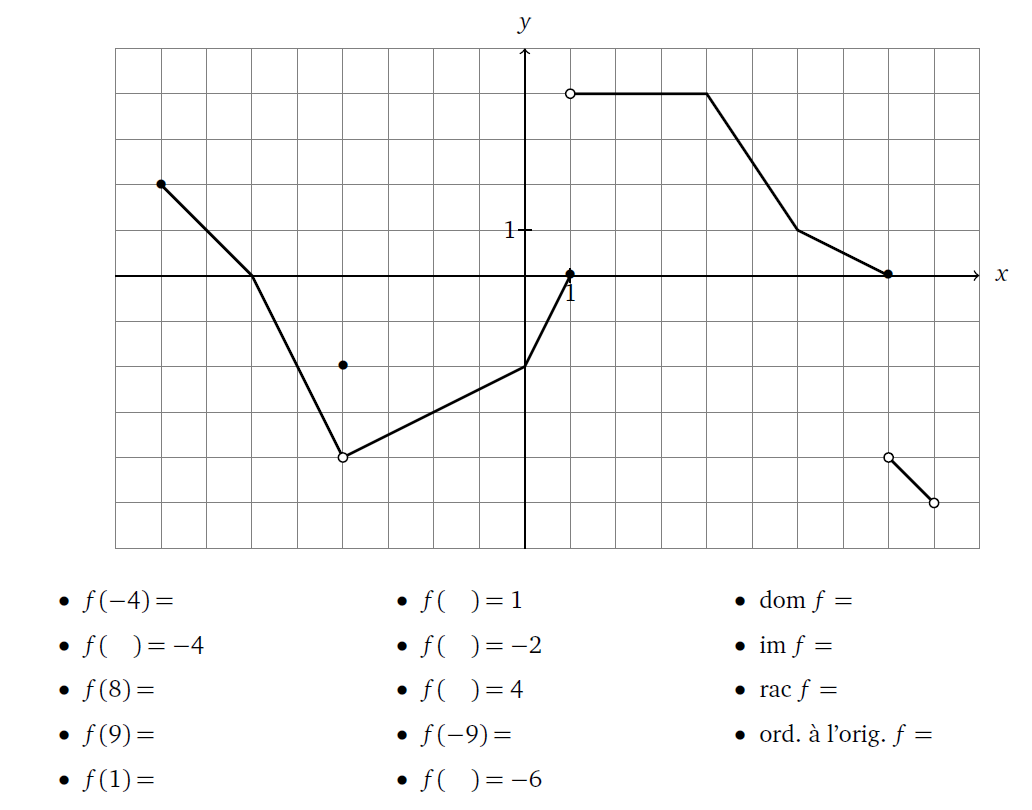
\includegraphics[scale=0.6]{qF.PNG} 
		Ensuite, donner la notation formelle de la fonction représentée (difficile !).
\end{exo}
\newpage
\begin{exo} \label{exof10c}
	En utilisant les règles de transformation de graphes, représenter les fonctions suivantes : \\
	\begin{enumerate}
		\item \begin{align*}
		f : {\rr} &\to \rr \\
		x &\mapsto 3\sqrt[3]{x+1}-2
		\end{align*} \\
		\item \begin{align*}
		f : {\rr} &\to \rr \\
		x &\mapsto (2x-7)^2
		\end{align*} \\
		\item \begin{align*}
		f : {\rr} \backslash \{7\} &\to \rr \\
		x &\mapsto \frac{2}{x-7}+\frac{1}{2}
		\end{align*} \\
		\item \begin{align*}
		f : {\rr} \backslash \{-3,2\} &\to \rr \\
		x &\mapsto 3|2x-1|+4
		\end{align*} \\
		\item \begin{align*}
		f : {\rr} \backslash \{-\frac{\pi}{3}\} &\to \rr \\
		x &\mapsto \frac{2x-1}{3x+\pi}
		\end{align*}
	
	\end{enumerate}
\end{exo}
\newpage
\begin{exo} \label{exof10d}
	Voici six fonctions et six graphes. Relier les six fonctions aux graphes correspondants. \\
	\begin{enumerate}
		
		\item ~~\\
		\begin{center}
			\begin{tikzpicture} [scale=0.8,domain=-5:5]
			\draw[step=1cm,gray,very thin] (-5,-5) grid (5,5);
			
			\draw[very thick,->] (-5,0) -- (5,0) node[anchor=south west] {x};
			\draw[very thick,->] (0,-5) -- (0,5) node[anchor=south west] {y};
			
			\foreach \x in {-5,-4,-3,-2,-1,0,1,2,3,4,5}
			\draw (\x cm,1pt) -- (\x cm,-1pt) node[anchor=north] {$\x$};
			\foreach \y in {-5,-4,-3,-2,-1,0,1,2,3,4,5}
			\draw (1pt,\y cm) -- (-1pt,\y cm) node[anchor=east] {$\y$};
			
			\draw[scale=1,domain=-2.16228:4.16228,smooth,variable=\x,blue] plot ({\x},{(\x-1)*(\x-1)*0.5});
			\end{tikzpicture}
		\end{center}
		
		\item ~~\\
		\begin{center}
			\begin{tikzpicture} [scale=0.8,domain=-5:5]
			\draw[step=1cm,gray,very thin] (-5,-5) grid (5,5);
			
			\draw[very thick,->] (-5,0) -- (5,0) node[anchor=south west] {x};
			\draw[very thick,->] (0,-5) -- (0,5) node[anchor=south west] {y};
			
			\foreach \x in {-5,-4,-3,-2,-1,0,1,2,3,4,5}
			\draw (\x cm,1pt) -- (\x cm,-1pt) node[anchor=north] {$\x$};
			\foreach \y in {-5,-4,-3,-2,-1,0,1,2,3,4,5}
			\draw (1pt,\y cm) -- (-1pt,\y cm) node[anchor=east] {$\y$};
			
			 \draw[color=blue,domain=-4.:5.,samples=900,scale=1] plot (\x,{-1*(sqrt(0.5 * \x +2))}) ;
			\end{tikzpicture}
		\end{center}
		\newpage
		\item ~~\\
		\begin{center}
			\begin{tikzpicture} [scale=0.9,domain=-5:5]
			\draw[step=1cm,gray,very thin] (-5,-5) grid (5,5);
			
			\draw[very thick,->] (-5,0) -- (5,0) node[anchor=south west] {x};
			\draw[very thick,->] (0,-5) -- (0,5) node[anchor=south west] {y};
			
			\foreach \x in {-5,-4,-3,-2,-1,0,1,2,3,4,5}
			\draw (\x cm,1pt) -- (\x cm,-1pt) node[anchor=north] {$\x$};
			\foreach \y in {-5,-4,-3,-2,-1,0,1,2,3,4,5}
			\draw (1pt,\y cm) -- (-1pt,\y cm) node[anchor=east] {$\y$};
			
			\draw[color=blue,domain=1.:4.0625,samples=500,scale=1] plot (\x,{-4*(sqrt(\x -1)) +2}) ;
			\end{tikzpicture}
		\end{center}
		
		\item ~~\\
		\begin{center}
				\begin{tikzpicture} [scale=0.9,domain=-5:5]
				\draw[step=1cm,gray,very thin] (-5,-5) grid (5,5);
				
				\draw[very thick,->] (-5,0) -- (5,0) node[anchor=south west] {x};
				\draw[very thick,->] (0,-5) -- (0,5) node[anchor=south west] {y};
				
				\foreach \x in {-5,-4,-3,-2,-1,0,1,2,3,4,5}
				\draw (\x cm,1pt) -- (\x cm,-1pt) node[anchor=north] {$\x$};
				\foreach \y in {-5,-4,-3,-2,-1,0,1,2,3,4,5}
				\draw (1pt,\y cm) -- (-1pt,\y cm) node[anchor=east] {$\y$};
				
				\draw[scale=1,domain=0.28571:5,smooth,variable=\x,blue] plot ({\x},{2 * ( \x )^(-1) -2});
				\draw[scale=1,domain=-5:-0.66667,smooth,variable=\x,blue] plot ({\x},{2 * ( \x )^(-1) -2});
				\end{tikzpicture}
		\end{center}		
		\newpage
		\item ~~\\
		\begin{center}
			\begin{tikzpicture} [scale=0.9,domain=-5:5]
			\draw[step=1cm,gray,very thin] (-5,-5) grid (5,5);
			
			\draw[very thick,->] (-5,0) -- (5,0) node[anchor=south west] {x};
			\draw[very thick,->] (0,-5) -- (0,5) node[anchor=south west] {y};
			
			\foreach \x in {-5,-4,-3,-2,-1,0,1,2,3,4,5}
			\draw (\x cm,1pt) -- (\x cm,-1pt) node[anchor=north] {$\x$};
			\foreach \y in {-5,-4,-3,-2,-1,0,1,2,3,4,5}
			\draw (1pt,\y cm) -- (-1pt,\y cm) node[anchor=east] {$\y$};
			
			\draw[scale=1,,domain=-5:5,smooth,variable=\x,blue] plot ({\x},{0.2 * (0.2 * \x)*(02  * \x) - 3});
			\end{tikzpicture}
		\end{center}
		
		\item ~~\\
		\begin{center}
			\begin{tikzpicture} [scale=0.9,domain=-5:5]
			\draw[step=1cm,gray,very thin] (-5,-5) grid (5,5);
			
			\draw[very thick,->] (-5,0) -- (5,0) node[anchor=south west] {x};
			\draw[very thick,->] (0,-5) -- (0,5) node[anchor=south west] {y};
			
			\foreach \x in {-5,-4,-3,-2,-1,0,1,2,3,4,5}
			\draw (\x cm,1pt) -- (\x cm,-1pt) node[anchor=north] {$\x$};
			\foreach \y in {-5,-4,-3,-2,-1,0,1,2,3,4,5}
			\draw (1pt,\y cm) -- (-1pt,\y cm) node[anchor=east] {$\y$};
			
			\draw[scale=1,domain=-5:5,smooth,variable=\x,blue] plot ({\x},{-2 * ( \x - 5.5)^(-1) -2});
			\end{tikzpicture}
		\end{center}	
	\end{enumerate}	
	\newpage
	\begin{enumerate}
		\item \begin{align*}
		f : {\rr}_{0}  &\to \rr \\
		x &\mapsto 2 (\frac{1}{x} -1)
		\end{align*}
		\item \begin{align*}
		f : {\rr} \backslash \left\{ \frac{11}{2} \right\}  &\to \rr \\
		x &\mapsto -2 \frac{1}{x - \frac{11}{2} } -2
		\end{align*}
		\item \begin{align*}
		f : {\rr}  &\to \rr \\
		x &\mapsto \frac{1}{5} \left(\frac{1}{5} x \right)^{2} - 3
		\end{align*}
		\item \begin{align*}
		f : {\rr}  &\to \rr \\
		x &\mapsto \frac{1}{2}(x-1)^{2}
		\end{align*}
		\item \begin{align*}
		f : [1,\infty[  &\to \rr \\
		x &\mapsto -4\sqrt{x -1} +2
		\end{align*}
		\item \begin{align*}
		f : [-4,\infty[  &\to \rr \\
		x &\mapsto -\sqrt{\frac{1}{2} x +2}
		\end{align*}
	\end{enumerate}
\end{exo}

\begin{exe} \label{exof10e}
	Supposons que dans quelques années, vous soyez devenu un chercheur en psychologie sociale. Vous souhaitez reproduire l'expérience de Asch\footnote{Solomon Asch est un des pionniers de la psychologie sociale, il a vécu du début à la fin du vingtième siècle.}, une expérience conçue pour étudier le phénomène du conformisme. L'expérience est la suivante : un interrogateur demande à un groupe de personnes d'enter dans une salle et leur montre à distance une image comme celle-ci :
	\begin{center}
	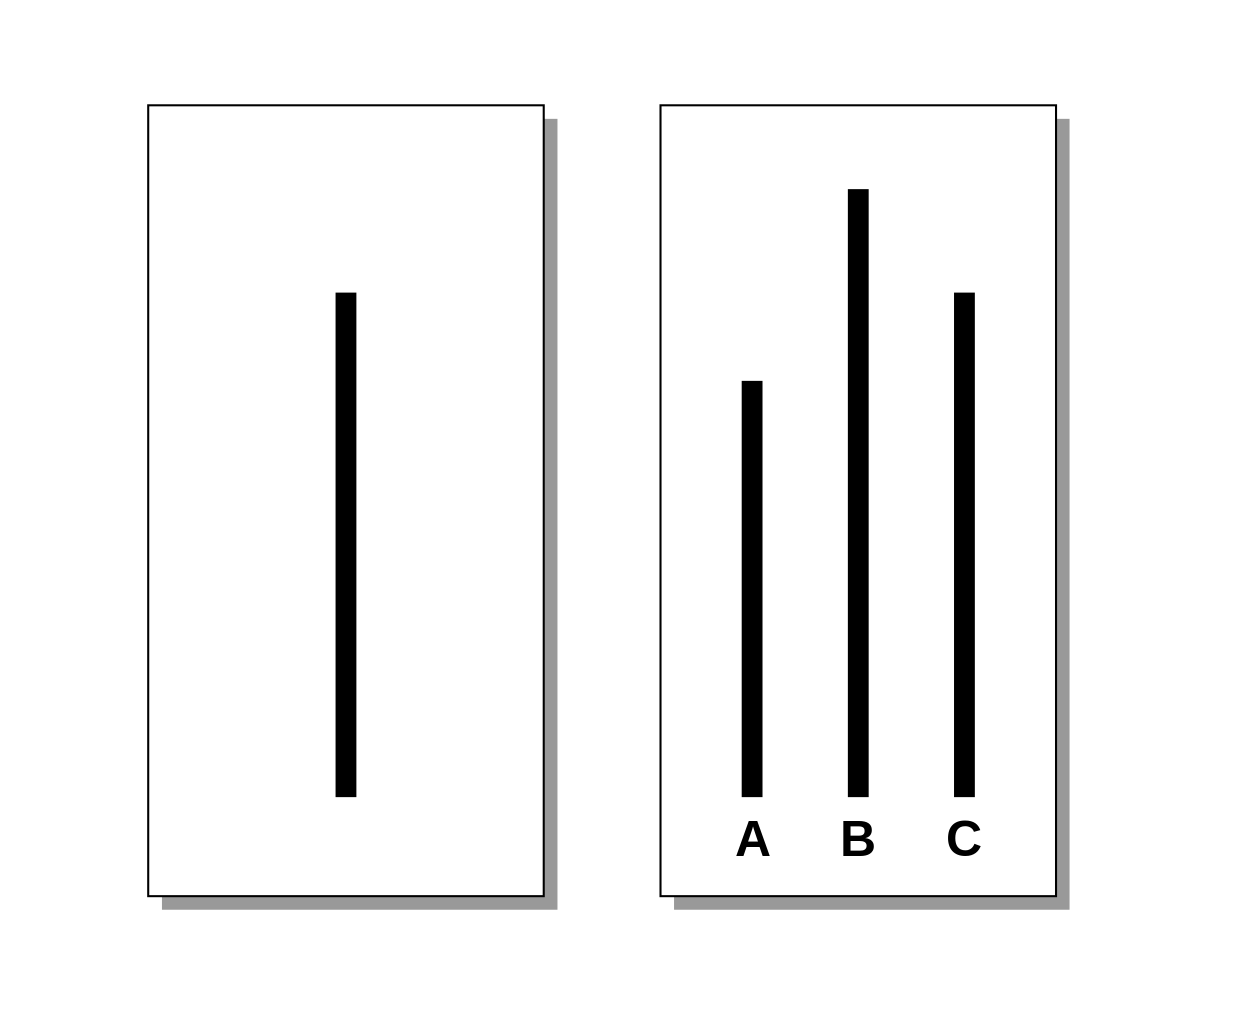
\includegraphics[scale=0.2]{Asch.PNG}
	\end{center}
	Ensuite, il demande aux personnes du groupe quelle est la barre de la boîte de droite qui est de la même taille que celle de la boîte de gauche. Le truc, c'est que dans le groupe des personnes interrogées, toutes les personnes sont complices avec l'interrogateur, sauf une. Tous ces complices vont d'abord hésiter, puis répondre $A$ (ce qui est évidemment une réponse incorrecte). Le but de l'expérience est de voir comment le sujet de l'expérience (la seule personne qui n'est pas complice avec l'interrogateur) va réagir : va-t-elle donner la bonne réponse évidente, ou va-t-elle se conformer au groupe et elle aussi répondre $A$ ? \\
	~~\\
	Dans votre cas, vous souhaitez voir comment la taille du groupe influence le pourcentage de sujets d'expérience qui se conforment au groupe. Imaginons que vous ayez récolté les données suivantes :
	\begin{center}
		\begin{tabular}{|c|c|c|c|c|}
			\hline
			Nombre de complices & $1$ & $2$ & $3$ & $5$ \\
			\hline
			Pourcentage de sujets d'expérience qui se conforment au groupe & $0$ & $13,6$ & $31,8$ & $58,3$\\
			\hline
		\end{tabular}
	\end{center}
	Afin d'étudier ces données, voici ce que je vous propose de faire :
	\begin{enumerate}
		\item Commencez par représenter ces données dans un repère approprié.
		\item Si vous deviez exprimer le pourcentage de sujets d'expérience qui se conforment au groupe en fonction du nombre de complices, quel type de fonction utiliseriez-vous ? Justifier votre choix.
		\item Déterminez l'expression d'une fonction qui modélise le lien entre le pourcentage de sujets d'expérience qui se conforment au groupe en fonction du nombre de complices à partir de vos données. Justifier votre choix.
		\item D'après votre modèle, estimez le pourcentage de sujets d'expérience qui se conformeraient au groupe s'il y avait $6$ complices.
		\item D'après votre modèle, estimez le pourcentage de sujets d'expérience qui se conformeraient au groupe s'il y avait $9$ complices. Cette estimation fait-elle sens ? Qu'est-ce que cela vous donne à penser au sujet de votre modèle ?
	\end{enumerate}
	Pour terminer : lorsque d'autres personnes ont réalisé cette expérience, elles ont observé qu'à partir d'environ $4$ complices, le pourcentage de sujets d'expérience qui se conforment au groupe n'augmente plus vraiment si on ajoute des complices et peut même diminuer à partir de $7$ ! Qu'est-ce que cela vous donne à penser au sujet de votre modèle ? Pouvez-vous imaginer une explication à ce phénomène ?
\end{exe}

\begin{exe} \label{exof10f}
	Supposons que dans quelques années, vous ayez fondé votre propre entreprise. Vous possédez $3$ usines qui fabriquent d'adorables ours en peluche. Puisque vous souhaitez rendre heureux le plus d'enfants possible\footnote{Et, anecdotiquement, maximiser votre profit.}, vous souhaitez trouver la vitesse optimale pour les machines de vos usines. Vous savez que vous pouvez les faire tourner plus rapidement que normalement, le seul problème est qu'au fur et à mesure qu'on augmente la vitesse des machines, de plus en plus de peluches sont défectueuses chaque jour et ne peuvent \sout{être vendues et vous rapporter de l'argent} rendre heureux des enfants. \\
	Après avoir mené quelques tests, vous avez les données suivantes :
	\begin{center}
		\begin{tabular}{|c|c|c|c|c|c|c|}
			\hline
			Vitesse des machines & $0$& $0.25$ & $0.5$ & $0.75$ & $1$ & $1.05$ \\
			\hline
			Nombre d'ours en peluches non défectueux & $0$ & $1680$ & $3021$ & $3934$ & $4492$ & $4571$ \\
			\hline
		\end{tabular}
	\end{center}
	\begin{center}
		\begin{tabular}{|c|c|c|c|c|c|c|}
			\hline
			Vitesse des machines & $1.1$ & $1.2$ & $1.3$ & $1.35$ & $1.4$ & $1.45$ \\
			\hline
			Nombre d'ours en peluches non défectueux & $4620$ & $4680$ & $4681$ & $4657$ & $4615$ & $4568$ \\
			\hline
		\end{tabular}
	\end{center}
	Afin de trouver la vitesse optimale à partir de ces données, voici ce que je vous propose de faire :
	\begin{enumerate}
		\item Commencez par représenter ces données dans un repère approprié.
		\item Si vous deviez exprimer le nombre d'ours en peluches non défectueux par heure en fonction de la vitesse des machines, quel type de fonction utiliseriez-vous ? Justifier votre choix.
		\item Déterminez l'expression d'une fonction qui modélise le lien entre le nombre d'ours en peluches non défectueux par heure en fonction de la vitesse des machines à partir de vos données. Justifier votre choix.
		\item D'après votre modèle, estimez la vitesse optimale.
		\item D'après votre modèle, à partir de quelle vitesse des machines la totalité des ours en peluche seront défectueux ?
	\end{enumerate}
\end{exe}

\begin{exo} \label{exof11}
	La fonction \begin{align*}
	f : {\rr}_{0} &\to \rr \\
	x &\mapsto \frac{1}{x}
	\end{align*}
	est-elle croissante ou décroissante ? Justifier.
\end{exo}

\begin{exo} \label{exof12}
	Parmi les fonctions de référence, déterminer celles qui sont (strictement) positive/négative, celles qui sont paires/impaires, celles qui sont (strictement) croissante/décroissante et celles qui sont majorée/minorée. Justifier à partir des définitions de ces propriétés.
\end{exo}

\begin{exo} \label{exof13}
	La fonction \begin{align*}
	f : \rr &\to \rr \\
	x &\mapsto x^3 - x^2
	\end{align*}
	est-elle croissante ou décroissante ? Justifier.
\end{exo}

\begin{exo} \label{exof14}
	La fonction \begin{align*}
	f : \rr &\to \rr \\
	x &\mapsto x^3 - x
	\end{align*}
	est-elle paire ou impaire ? Justifier.
\end{exo}

\begin{exo} \label{exof15}
	La fonction \begin{align*}
	f : {\rr}_{0} &\to \rr \\
	x &\mapsto \frac{-x^2+6}{\pi x^5 +x}
	\end{align*}
	est-elle paire ou impaire ? Justifier.
\end{exo}

\begin{exo} \label{exof16}
	Une fonction paire peut-elle être croissante ? Strictement croissante ?
\end{exo}

\begin{exo} \label{exof17}
	La fonction \begin{align*}
	f : {\rr} \backslash \{0\} &\to \rr \\
	x &\mapsto -x^2 + \frac{1}{-4|x|}
	\end{align*}
	est-elle majorée ou minorée ? Justifier.
\end{exo}

\begin{exo} \label{exof18}
	La fonction \begin{align*}
	f : \nn &\to \rr \\
	x &\mapsto \frac{1}{x+1}
	\end{align*}
	est-elle majorée ou minorée ? Justifier.
\end{exo}

\begin{exo} \label{exof19}
	La somme de deux fonctions croissantes est-elle (nécessairement) une fonction croissante ? La produit de deux fonctions croissantes est-il (nécessairement) une fonction croissante ? La composée de deux fonctions croissantes est-elle (nécessairement) une fonction croissante ? 
\end{exo}

\begin{exo} \label{exof20}
	La somme de deux fonctions décroissantes est-elle (nécessairement) une fonction décroissante ? La produit de deux fonctions croissantes est-il (nécessairement) une fonction décroissante ? La composée de deux fonctions décroissantes est-elle (nécessairement) une fonction croissante ? 
\end{exo}

\begin{exo} \label{exof21}
	La somme de deux fonctions paires est-elle (nécessairement) une fonction paire ? La produit de deux fonctions paires est-il (nécessairement) une fonction paire ? La composée de deux fonctions paires est-elle (nécessairement) une fonction paire ? 
\end{exo}

\begin{exo} \label{exof22}
	La somme de deux fonctions impaires est-elle (nécessairement) une fonction impaire ? La produit de deux fonctions impaires est-il (nécessairement) une fonction impaire ? La composée de deux fonctions impaires est-elle (nécessairement) une fonction impaire ? 
\end{exo}

\begin{exo} \label{exof23}
	La somme de deux fonctions majorées est-elle (nécessairement) une fonction majorée ? La produit de deux fonctions majorées est-il (nécessairement) une fonction majorée ? La composée de deux fonctions majorées est-elle (nécessairement) une fonction majorée ? 
\end{exo}

\begin{exo} \label{exof24}
	La somme de deux fonctions minorées est-elle (nécessairement) une fonction minoréee ? La produit de deux fonctions minorées est-il (nécessairement) une fonction minorée ? La composée de deux fonctions minorées est-elle (nécessairement) une fonction minorée ? 
\end{exo}
\newpage
\begin{exo} \label{exof26}
	~~\\ ~~\\	
	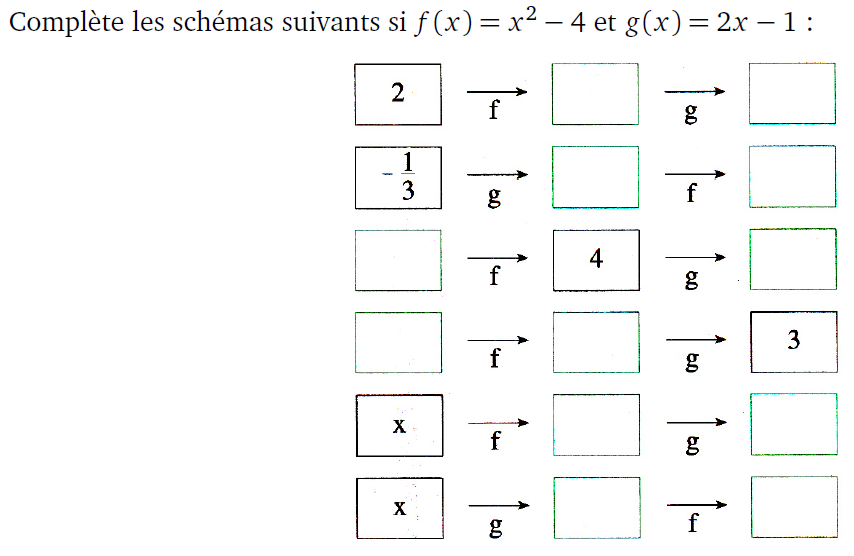
\includegraphics[scale=0.6]{qC.PNG}
\end{exo}

\begin{exo} \label{exof27}
 Décomposer les fonctions suivantes à partir des fonctions de référence.
 Exemple :
 	\item \begin{align*}
 	f : \rr \backslash \{-1\} &\to \rr \\
 	x &\mapsto \frac{1}{x+1} + \sqrt{x}
 	\end{align*}
 Une décomposition de $f$ à partir des fonctions de référence est la suivante : $f = (g \circ (h + i)) + j$ avec $g$ la fonction inverse, $h$ la fonction identité, $h$ la fonction constante de constante $1$ et $j$ la fonction racine carrée. \\
 ~~\\
 \begin{enumerate}
 	\item \begin{align*}
 	f : \rr \backslash \{-1\} &\to \rr \\
 	x &\mapsto 3(x+|x|)^3
 	\end{align*}
 	\item \begin{align*}
 	f : {\rr}_{0} &\to \rr \\
 	x &\mapsto \frac{2+x^2}{x}
 	\end{align*}
 	\item \begin{align*}
 	f : \rr &\to \rr \\
 	x &\mapsto 3x^2 + \sqrt[3]{x}(x^2-\pi)
 	\end{align*}
 \end{enumerate}
\end{exo}

\begin{exo} \label{exof28}
 Pour chaque couple de fonctions suivants, déterminer les domaines de définition des fonctions $f+g$, $\frac{f}{g}$, $f \circ g$ et $g\circ f$ ainsi que leur expression algébrique.
  \begin{enumerate}
  	\item \begin{align*}
  	f : [-\frac{1}{2},\infty] &\to \rr \\
  	x &\mapsto \sqrt{2x+1}
  	\end{align*}
  	et
  	\begin{align*}
  	g : \rr &\to \rr \\
  	x &\mapsto \pi - x^2
  	\end{align*}
  	\item \begin{align*}
  	f : \rr &\to \rr \\
  	x &\mapsto |x^3-3|
  	\end{align*}
  	et
  	\begin{align*}
  	g : {\rr}_{0} &\to \rr \\
  	x &\mapsto \frac{1}{x}+x
  	\end{align*}
  \item \begin{align*}
  f : {\rr}_{0} &\to \rr \\
  x &\mapsto \sqrt[3]{-x^2+\frac{1}{x^2}}
  \end{align*}
  et
  \begin{align*}
  g : \{0\} &\to \rr \\
  x &\mapsto 2\sqrt{-|x|+\frac{2}{7}x}
  \end{align*}
\end{enumerate}
\end{exo}

\begin{exo} \label{exof25}
	\url{https://www.auto-math.be/public/0/module/13}
\end{exo}

\chapter{Solutions}

Lorsqu'un exercice est composé d'une série de sous-exercices, seule la solution du premier sous-exercice est accompagnée du développement.
\section{Les équations et les inéquations : solutions}

\begin{exo}
	\begin{enumerate}
		\item $\left\{ \frac{5 + 7\sqrt{3} \pi}{(\sqrt{3}-4)\pi} \right\}$. Développement : 
		$$\frac{5}{\pi} +4x = \sqrt{3}(x-7)$$
		Par distributivité (membre de droite de l'équation) :
		$$\frac{5}{\pi} +4x = \sqrt{3}x-\sqrt{3}.7$$
		Par la règle $5$ (voir section \ref{sectionequation}), avec $c = \frac{5}{\pi}$ :
		$$\frac{5}{\pi} +4x -  \frac{5}{\pi} = \sqrt{3}x-\sqrt{3} . 7 -  \frac{5}{\pi}$$
		Par commutativité de la somme (membre de gauche) :
		$$4x + \frac{5}{\pi} -  \frac{5}{\pi} = \sqrt{3}x-\sqrt{3} . 7 -  \frac{5}{\pi}$$
		$$4x=\sqrt{3}x-\sqrt{3} . 7 -  \frac{5}{\pi}$$
		Par la règle $5$, avec $c = \sqrt{3}x$ :
		$$4x-\sqrt{3}x=\sqrt{3}x-\sqrt{3}.7 -  \frac{5}{\pi}-\sqrt{3}x$$
		Par distributivité (membre de gauche) et par commutativité de la somme (membre de droite) :
		$$(4-\sqrt{3})x=\sqrt{3}x-\sqrt{3}x-\sqrt{3}.7 -  \frac{5}{\pi}$$
		$$(4-\sqrt{3})x=-\sqrt{3}.7 -  \frac{5}{\pi}$$
		Par la règle $7$, avec $c = (4-\sqrt{3})$ :
		$$\frac{(4-\sqrt{3})x}{4-\sqrt{3}}=\frac{-\sqrt{3}.7 -  \frac{5}{\pi}}{4-\sqrt{3}}$$
		Par commutativité de la somme et du produit (membre de gauche) :
		$$x=\frac{5 + 7\sqrt{3} \pi}{(\sqrt{3}-4)\pi}$$
		~~\\
		(Note : on comprend pourquoi on ne justifie pas chaque étape de nos calculs en général, c'est beaucoup trop lourd et abolument pas nécessaire une fois qu'on a appris à utiliser les règles de calcul de façon correcte. Au passage, faisons remarquer que dans la correction ci-dessus, on a (volontairement) passé sous silence les emplois de l'associativité de la somme et du produit, sans quoi la réponse serait encore plus longue).
		\item $\{ 0,7 \}$
		\item $\{ 0 \}$
	\end{enumerate}
\end{exo}

\begin{exo}
	Puisque $a=b$, on a $a-b=0$. Pour passer de la quatrième ligne à la cinquième ligne, on divise donc par $0$, ce qui est illégitime.
\end{exo}

\begin{exo}
	Notons $x$ la note qu'il doit obtenir pour avoir une moyenne de $80$. $x$ vérifie l'équation :
	$$\frac{75+82+71+84+x}{5}=80$$
	\'Equation qui a pour solution $88$. Il doit donc obtenir $88$ s'il souhaite avoir une moyenne de $80$.
\end{exo}

\begin{exo}
	Notons $x$ le nombre d'enfants dans la salle. S'il y avait $x$ enfants dans la salle, il devait y avoir $600-x$ adultes dans la salle, qui ont chacun payé $8${\euro}, tandis que les $x$ enfants ont chacun payé $5${\euro}, pour un total de $4155${\euro} :
	$$x.5+(600-x).8=4155$$
	\'Equation qui a pour solution $215$. Il y avait donc $215$ enfants dans la salle.
\end{exo}

\begin{exo}
	Notons $x$ la longueur du côté adjacent.
	\begin{enumerate}
		\item Dans ce cas, la longueur du côté parallèle à la rivière est de $2x$ et l'aire de la surface cloturée est de $x.2x$. Par ailleurs, puisque le pourtour de la surface a une longueur de $180$ m, on a l'équation : $x + 2x + x + 2x = 180$, équation qui a pour solution $30$. L'aire de la surface cloturée est donc de $30.2.30=1800$ m$^{2}$.
		\item Dans ce cas, la longueur du côté parallèle à la rivière est de $\frac{3}{2}x$ et l'aire de la surface cloturée est de $x.\frac{3}{2}x$. Par ailleurs, puisque le pourtour de la surface a une longueur de $180$ m, on a l'équation : $x + \frac{3}{2}x + x + \frac{3}{2}x = 180$, équation qui a pour solution $36$. L'aire de la surface cloturée est donc de $36.\frac{3}{2}.36=1944$ m$^{2}$.
		\item égale à la longueur du côté adjacent. Dans ce cas, la longueur du côté parallèle à la rivière est de $x$ et l'aire de la surface cloturée est de $x.x$. Par ailleurs, puisque le pourtour de la surface a une longueur de $180$ m, on a l'équation : $x + x + x + x = 180$, équation qui a pour solution $45$. L'aire de la surface cloturée est donc de $45.45=2025$ m$^{2}$.
	\end{enumerate}
\end{exo}

\begin{exo}
	Le salaire horaire de base d'un travailleur est de $10${\euro}, mais il reçoit une fois et demi son salaire pour chaque heure supplémentaire fournie en plus des $40$ heures hebdomadaires. S'il reçoit $595${\euro} pour la semaine, combien d'heures supplémentaires a-t-il effectuées ?
	Notons $x$ le nombres d'heures supplémentaires effectuées. En travaillant ses $40$ heures de base, il a gagné $40.10=400${\euro}. Ses heures supplémentaires lui ont rapporté $x.\frac{3}{2}.10${\euro}. La somme de ces deux nombres donne $595${\euro} :
	$$400 + 15x = 595$$
	Cette équation a pour solution $13$. Il a donc effectué $13$ heures supplémentaires.
\end{exo}

\begin{exo}
	\begin{enumerate} \item $\{ \frac{6328}{81} \}$. Développement : \\$$\frac{7x}{3}-\frac{3}{2}(100-\frac{2x}{7}) = \frac{x}{2} + \frac{x+2}{3}$$
		$$\frac{7x}{3}-150 + \frac{3x}{7} = \frac{3x}{6} + \frac{2x+4}{6}$$
		$$\frac{7x.7.2}{3.7.2}-\frac{150.3.7.2}{3.7.2} + \frac{3x.3.2}{7.3.2} = \frac{3x.7}{6.7} + \frac{(2x+4).7}{6.7}$$
		$$(7.7.2)x-150.3.7.2 + (3.3.2)x = 3x.7 + (2x+4).7$$
		$$(7.7.2 + 3.3.2 - 3.7 - 2.7)x=150.3.7.2+4.7$$
		$$x=\frac{150.3.7.2+4.7}{7.7.2 + 3.3.2 - 3.7 - 2.7}$$
		$$x=\frac{6328}{81}$$
		\item $\{ -\frac{1}{30} \}$
		\item $\{ -8,8 \}$
		\item $\{ 3 \}$
		\item $\emptyset$
		\item $\{ -4,2 \}$
		\item $\{ -1 \}$
	\end{enumerate}
\end{exo}

\begin{exo} \begin{enumerate}
		\item $\{ \frac{15 - \sqrt{41}}{4},\frac{15 + \sqrt{41}}{4} \}$. Développement : \\
		$$\frac{4x+5}{8x^2-18x-35} - \frac{x}{x-1} = \frac{5}{2x-7}-3\frac{x-2}{x-1}$$
		On remarque que $x$ doit être différent de $-\frac{5}{4}$, $\frac{7}{2}$, et $1$ pour que l'équation fasse sens (conditions d'existence). On suppose donc que $x \notin \{ -\frac{5}{4}, \frac{7}{2} , 1 \}$.
		$$\frac{4x+5}{(4x+5)(2x-7)} - \frac{x}{x-1} = \frac{5(x-1)}{(2x-7)(x-1)}-3\frac{(x-2)(2x-7)}{(x-1)(2x-7)}$$
		$$\frac{(x-1)}{(2x-7)(x-1)} - \frac{x(2x-7)}{(x-1)(2x-7)} = \frac{5(x-1)}{(2x-7)(x-1)}-3\frac{(x-2)(2x-7)}{(x-1)(2x-7)}$$
		$$x-1 - (2x^2 - 7x) = 5x - 5 - (6x^2 - 12 x - 21x + 42)$$
		$$-2x^2 + 8x - 1 = -6x^2 +38x - 47$$
		$$4x^2 - 30x + 46 = 0$$
		$$4\left(x^2 - \frac{15}{2}x + \frac{23}{2}\right) = 0$$
		$$\left(x - \left(\frac{15 - \sqrt{41}}{4}\right)\right)\left(x -\left(\frac{15 + \sqrt{41}}{4}\right)\right) = 0$$
		\item $\{ 5-2\sqrt{5},5+2\sqrt{5} \}$
		\item $\{ \frac{8}{3} \}$
		\item $\{ \frac{49 - \sqrt{2377}}{12},\frac{49 + \sqrt{2377}}{12} \}$
		\item $\{ 34,38 \}$
		\item $\{ -1,1,2 \}$
		\item $\{ -1 \}$
		\item $\{ 3,7 \}$
		\item $\emptyset$
		\item $\{ -2,-1,2 \}$
		\item $\{ \frac{-13 - \sqrt{5}}{2},\frac{-13 + \sqrt{5}}{2} \}$
		\item $\{ -\sqrt{25+\frac{60}{\pi}},\sqrt{25+\frac{60}{\pi}} \}$
		\item $\{ -\frac{1}{7},5 \}$
		\item $\{ 0 \}$
		\item $\{ 1,\sqrt[5]{3} \}$
		\item $\{ -\frac{2}{3},\frac{2}{5} \}$
		\item $\{ 2+\sqrt{6},-1-\sqrt{7} \}$
		\item $\emptyset$
	\end{enumerate}
\end{exo}

\begin{exo}
	Solutions sur le site web.
\end{exo}

\begin{exo}
	\begin{enumerate}
		\item $[-2, 2]$. Développement : \\
		$$x^2 \le 4$$
		Par la règle $4$ (voir section \ref{sectioninequation}), avec $c=4$ :
		$$x^2 - 4 \le 0$$
		Par distributivité :
		$$(x+2) (x-2) \le 0$$
		Tableau de signes : \\
		\begin{tikzpicture}
		\tkzTabInit{$x$ / 1 , $(x+2)$ / 1 , $(x-2)$ / 1 , $(x+2) (x-2)$ / 1}{$-\infty$, $-2$, $2$, $+\infty$}
		\tkzTabLine{ , -, 0, +, 4 , +, }
		\tkzTabLine{ , -, -4, -, 0 , +, }
		\tkzTabLine{ , +, 0, -, 0 , +, }
		\end{tikzpicture} \\
		~~\\
		Les solutions de l'inéquation sont donc les éléments de $[-2, 2]$.
		\item $]-\infty, -\frac{12}{11}[$
		\item $]-\infty, 0[ \cup  ]0, 1]$
		\item $\emptyset$
	\end{enumerate}
\end{exo}

\begin{exo} Soit $x$ le nombre de kilomètres que vous allez parcourir. On se demande pour quel valeur de $x$ le coût de Ismaël ($125+(1,50)x$) sera plus petit que celui de Jean-Claude ($110+(1,75)x$). On a donc une inéquation :
	$$125+(1,50)x < 110+(1,75)x$$
	Les solutions de cette inéquation sont les éléments de $]60, \infty[$. Ismaël est donc plus avantageux que Jean-Claude à partir de $60$ kilomètres.
\end{exo}

\begin{exo} Vraisemblablement, si on fait tourner la machine à une vitesse $x$, elle produit $3x^2$ donuts par minutes. On cherche les valeurs de $x$ pour lesquels le nombre de donuts produits par minute est inférieur ou égal à $60$ :
	$$3x^2 \le 60$$
	Cette inéquation a pour solutions les éléments de $[-2 \sqrt{5}, 2 \sqrt{5}]$. La vitesse maximale à laquelle on peut pousser la machine est donc $2 \sqrt{5}$ fois sa vitesse normale.
\end{exo}

\begin{exo} On a l'inéquation :
	$$4\pi r^2 > \frac{4}{3} \pi r^3$$
	Dans ${{\rr}_{0}}^{+}$ (un rayon est toujours strictement positif, inutile donc de considérer les solutions négatives de cette inéquation), cette inéquation a pour solutions les éléments de $]0, 3[$. \\
	Conclusion pour les boulettes ; le rayon ne doit pas dépasser $3$ cm !\footnote{Bon, pour dire vrai, cette conclusion n'a pas beaucoup de sens. En effet, cet exercice vous demande de comparer la valeur numérique d'une aire avec celle d'un volume, c'est un peu comme comparer un nombre de pommes avec un nombre de poires. Par ailleurs, les unités qu'on utilise (par exemple : cm ou m ?) vont beaucoup influencer le sens de la conclusion, au point de la rendre non pertinente. Mais je vous conseille malgré tout de ne pas faire des boulettes trop grosses, c'est meilleur.}
\end{exo}

\begin{exo} ~~\\
	\begin{enumerate}
		\item $]-\infty, 0[$. Développement :
		$$\frac{-x^2-5}{2x} \ge 0$$
		On remarque que l'expression ne fait sens que si $x \in {\rr}_{0}$ (conditions d'existence).
		$$\frac{-x^2-5}{x} \ge 0$$
		Deux possibilités, si $x < 0$, on doit alors modifier le sens de l'inégalité lorsqu'on multiplie par $x$ :
		$$\frac{-x^2-5}{x}.x \le 0.x$$
		$$-x^2-5 \le 0$$
		$$-1.(-x^2-5) \ge -1.0$$
		$$x^2+5 \ge 0$$
		$$x^2 \ge -5$$
		Tous les nombres réels $x$ sont tels que $x^2 \ge -5$. Il n'y a pas de condition. Tous les nombres de $]-\infty, 0[$ vérfient donc l'inéquation. \\
		À présent, vérifions la deuxième possibilité : si $x \ge 0$, alors on ne doit pas modifier le sens de l'inégalité lorsqu'on multiplie par $x$ :
		$$\frac{-x^2-5}{x}.x \ge 0.x$$
		$$-x^2-5 \ge 0$$
		$$-1.(-x^2-5) \le -1.0$$
		$$x^2+5 \le 0$$
		$$x^2 \le -5$$
		Aucun nombres réels $x$ est tel que $x^2 \le -5$. Aucun nombre de $[0,\infty[$ ne vérifie donc l'inéquation. \\
		En conclusion, l'ensemble des solutions de l'inéquation est $]-\infty, 0[$. 
		\item $]-\infty,-2[ \cup ]-2, 0[$
		\item $]1, 9]$
		\item $]-\infty, 0] \cup [\frac{1}{3} (3 - \sqrt{6}), \frac{1}{3} (3 + \sqrt{6})]$
		\item $\emptyset$
		\item $]-\infty, -2[ \cup ]1, \frac{5}{2}[$
		\item $]-\infty, -\frac{3}{2}[ \cup ]0, \infty[$
		\item $]0,\frac{1}{2}[$
		\item $\{ -\frac{4}{3} \}$
		\item $[0,\infty[$
	\end{enumerate}
\end{exo}

\begin{exo}
	Solutions sur le site web.
\end{exo}

\section{Les polynômes, les droites et les paraboles : solutions}

\begin{exo}
	\begin{enumerate} ~~\\
		\item Oui. Il s'agit d'une somme avec un unique terme qui est un produit d'une puissance entière de la variable $x$ (ici : $1$) par un nombre réel (ici : $1$).
		\item Oui.
		\item Oui.
		\item Non.
		\item Oui.
		\item Non.
		\item Non.
		\item Non.
		\item Oui.
	\end{enumerate}
\end{exo}

\begin{exo}
	Vérifier si les nombres donnés sont des racines des polynômes proposés.
	\begin{enumerate}
		\item Non : $3^2 +7.3 -1 = 9 +21 - 1 = 29 \neq 0$.
		\item Oui.
		\item Oui (tous les nombres sont racines du polynôme nul).
		\item Oui.
		\item Oui.
	\end{enumerate}
\end{exo}

\begin{exo}  ~~\\ \begin{enumerate}
		\item $x^{12} - x^2 + 7x + (\pi -1)$. Développement : \\
		$x^2+7x-1 + x^{12} + \pi -x^2 = x^{12} - x^2 + 7x + (\pi -1)$
		\item $x^7 - x^4 +1200x+3$.
	\end{enumerate}
\end{exo}
\newpage
\begin{exo}  ~~\\ \begin{enumerate}
		\item $\frac{1}{7}x^{11} -x^{10} + \pi x^{9} +\frac{\sqrt[3]{3}}{7}x^3 -\sqrt[3]{3}x^2 + \pi \sqrt[3]{3} x$. Développement :
		\begin{align*}
		(-\frac{1}{7}x^2+x-\pi).(-x^{9} -\sqrt[3]{3}x) =& -\frac{1}{7}x^2.(-x^{9}) -\frac{1}{7}x^2.(-\sqrt[3]{3}x) \\
		&+ x.(-x^{9}) + x.(-\sqrt[3]{3}x) \\
		&-\pi.(-x^{9}) -\pi.(-\sqrt[3]{3}x) \\
		=&\frac{1}{7}x^{11} +\frac{\sqrt[3]{3}}{7}x^3 \\
		&+ -x^{10} -\sqrt[3]{3}x^2 \\
		&+\pi x^{9} + \pi \sqrt[3]{3} x \\
		=&\frac{1}{7}x^{11} -x^{10} + \pi x^{9} +\frac{\sqrt[3]{3}}{7}x^3 -\sqrt[3]{3}x^2 + \pi \sqrt[3]{3} x
		\end{align*}
		\item $-6 x^{10} + 18 x^7 - 1200 x^5 - x^4 + 3600 x^2 + 3 x$.
	\end{enumerate}
\end{exo}

\begin{exo}
	Parmi les couples de polynômes suivants, dans quels cas la division du premier par la deuxième est-elle possible ? Justifier.
	\begin{enumerate}
		\item $x^2+2x+1$ et $x^{2} +1$. Possible car le degré du premier polynôme ($2$) est plus grand ou égal au degré du second ($2$).
		\item Impossible.
		\item Posible. $4 = \frac{4}{3}.3 + 0$
		\item Possible. $x^4 - \sqrt{11} x^3 + x^2 - 13 x + 1 = (x^3 + (-2 - \sqrt{11}) x^2 + (5 + 2 \sqrt{11}) x - 4 \sqrt{11} - 23). (x + 2) + 47 + 8 \sqrt{11}$.
		\item Impossible.
		\item Possible. $-4x^3 +x^2 +5203 = (-4 x^2 - 43 x - 473)(x-11)+0$.
	\end{enumerate}
\end{exo}

\begin{exo}
	Solutions sur le site web.
\end{exo}

\begin{exo}
	Une définition possible est la suivante : \\
	Une \emph{droite verticale} est un ensemble de points $(x,y)$ du plan ${\rr}^2$ qui vérifie une équation du type $x = a$ où $a$ est un nombre réel.
	La définition \ref{défdroite} ne permet pas de parler de droite verticale car la variable $y$ doit être présente dans le membre de gauche de l'équation cartésienne d'une droite (non-verticale) selon la définition \ref{défdroite}. Il n'est pas vraiment pertinent de parler de la pente d'une droite verticale, mais certaines personnes disent qu'une droite verticale a \og une pente infinie \fg{}. Je vous déconseille vivement d'utiliser ce type d'expression.
\end{exo}

\begin{exo}
	Donner l'équation cartésienne d'une droite...
	\begin{enumerate}
		\item $y=3x-100$. Développement : \\
		L'équation cartésienne est du type $y=ax+b$ où $a,b \in \rr$, avec $a$ la pente de la droite et $b$ l'ordonnée à l'origine de la droite. L'équation cartésienne d'une droite de pente $3$ et d'ordonnée à l'origine $-100$ est donc $y=3x-100$.
		\begin{center}
			\begin{tikzpicture}
			\begin{axis}[ xmin=-250, xmax=250, ymin=-250, ymax=250, extra x ticks={-200,-150,-100,-50,0,50,100,150,200}, extra y ticks={-200,-150,-100,-50,0,50,100,150,200}, extra tick style={grid=major}, ]
			\addplot[color=black] coordinates { (0,-250) (0,-200) (0,-150) (0,-100) (0,-50) (0,0) (0,50) (0,100) (0,150) (0,200) (0,250) };
			\addplot[color=black] coordinates { (-250,0) (-200,0) (-150,0) (-100,0) (-50,0) (0,0) (50,0) (100,0) (150,0) (200,0) (250,0) };
			\addplot[color=blue] coordinates { (-50,-250) (0,-100) (50,50) (100,200) (116.66,250) };
			\end{axis}
			\end{tikzpicture}
		\end{center}
		\item $y=-\frac{1}{\pi}x-6$
		\item $y=-6$.
		\item $y=4x$
		\item $y= -\frac{3}{5}x+3$
		\item $y=\frac{8}{5}x - \frac{11}{5}$
		\item $y=-\frac{8}{5}x - \frac{11}{5}$
		\item $y=-\frac{1}{3}x+\frac{2}{3}$
		\item $y=-\frac{1}{-\frac{\sqrt{2}}{2}}x + 7=\frac{2}{\sqrt{2}}x + 7 = \sqrt{2}x + 7$
		\item $y=\frac{2}{3}x+\frac{4}{3}$
		\item $y=-\frac{1}{5}x+\frac{7}{5}$
	\end{enumerate}
\end{exo}

\begin{exo}
	En quel point coupe l'axe des ordonnées une droite qui passe par le point $(2,1)$ et parallèle à une autre droite, qui elle coupe l'axe des abscisses en $-4$ et est parallèle à une troisième droite passant par le point $(-1,1)$ et d'ordonnée à l'origine $-1$ ? Représenter les trois droites sur un graphique.
	Désignons par $d_1$ la première droite (celle dont on cherche l'ordonnée à l'origine), $d_2$ la deuxième (qui est celle par rapport à laquelle $d_1$ est parallèle) et $d_3$ la troisième (qui est celle passant par le point $(-1,1)$ et d'ordonnée à l'origine $-1$). \\
	Commençons par déterminer l'équation cartésienne de $d_3$. Puisqu'elle passe par les points $(0,-1)$ et $(-1,1)$, sa pente est égale à $\frac{-1-1}{0-(-1)}=-2$. Son équation cartésienne est donc de la forme $y=-2x+b$, avec $b \in \rr$. Pour trouver le $b$, on peut remplacer $x$ et $y$ par $-1$ et $1$ par exemple (puisque $d_3$ passe par $(-1,1)$) : $1=-2.(-1) + b$, donc $b=-1$. \\
	Passons à l'équation cartésienne de $d_2$. Puisqu'elle est parallèle à $d_3$, sa pente est égale à $-2$. Son équation cartésienne est donc de la forme $y=-2x+b$, avec $b \in \rr$. Pour trouver le $b$, on peut remplacer $x$ et $y$ par $-4$ et $0$ (puisque $d_3$ coupe l'axe des abscisses en $-4$) : $0=-2.(-4)+b$, donc $b=-8$. \\
	Enfin, trouvons l'équation cartésienne de $d_1$. Puisqu'elle est parallèle à $d_2$, sa pente est égale à $-2$. Son équation cartésienne est donc de la forme $y=-2x+b$, avec $b \in \rr$. Pour trouver le $b$, on peut remplacer $x$ et $y$ par $2$ et $1$ (puisque $d_1$ passe par $(2,1)$) : $2=-2.1+b$, donc $b=4$. \\
	On peut à présent représenter les trois droites : en bleu, $d_1$, en rouge, $d_2$, en vert, $d_3$. \\
	\begin{center}
		\begin{tikzpicture}
		\begin{axis}[ xmin=-5, xmax=5, ymin=-5, ymax=5, extra x ticks={-4,-3,-2,-1,0,1,2,3,4}, extra y ticks={-4,-3,-2,-1,0,1,2,3,4}, extra tick style={grid=major}, ]
		\addplot[color=black] coordinates { (0,-5) (0,-4) (0,-3) (0,-2) (0,-1) (0,0) (0,1) (0,2) (0,3) (0,4) (0,5) };
		\addplot[color=black] coordinates { (-5,0) (-4,0) (-3,0) (-2,0) (-1,0) (0,0) (1,0) (2,0) (3,0) (4,0) (5,0) };
		\addplot[color=blue] coordinates { (-0.5,5) (4.5,-5) };
		\addplot[color=red] coordinates { (-5,2) (-1.5,-5) };
		\addplot[color=green] coordinates { (-3,5) (2,-5) };
		\end{axis}
		\end{tikzpicture}
	\end{center}
\end{exo}

\begin{exo} ~~\\
	\begin{enumerate}
		\item La droite doit donc passer par le point $(0,-5)$. L'équation suivante doit donc être vérifiée : $-5=(n-5)0+(-n+1)=-n+1$. Autrement dit, $n$ doit être égal à $-6$.
		\item soit perpendiculaire à une droite passant par les point $(1,5)$ et $((-1,-1)$. Une telle droite a comme pente $\frac{5-(-1)}{1-(-1)}=\frac{6}{2}=3$. Si on souhaite qu'une droite d'équation cartésienne $y=(n-5)x+(-n+1)$ soit perpendiculaire à cette droite, il faut que sa pente soit égale à $-\frac{1}{3}$, autrement dit que $n-5=-\frac{1}{3}$. En conclusion, $n$ doit donc être égal $-\frac{1}{3}+5=\frac{14}{3}$.
	\end{enumerate}
\end{exo}

\begin{exo}
	Solutions sur le site web.
\end{exo}

\begin{exo} ~~\\
	Si $\Delta > 0$, la parabole coupe l'axe des abscisses en deux points. \\
	Si $\Delta = 0$, le sommet de la parabole se trouve sur l'axe des abscisses. \\
	Si $\Delta < 0$, la parabole se trouve strictement en dessous ou strictement au dessus de l'axe des abscisses.
\end{exo}

\begin{exo}
	Déterminer si les paraboles suivantes ont des intersections avec l'axe des abscisses. Si oui, donner leurs coordonnées.
	\begin{enumerate}
		\item Chercher les intersections de cette parabole avec l'axe des abscisses revient à chercher les nombres réels $x$ tels que $3x^2-x+\frac{7}{3}=0$, autrement dit les racines du polynôme $3x^2-x+\frac{7}{3}$. Par le théorème \ref{thépara}, puisque $\Delta = 1 - 4.3.\frac{7}{3} = -27$, ce polynôme n'a pas de racine.
		\item Oui. $(-\frac{5}{2} - \frac{\sqrt{5}}{2},0)$ et $(\frac{5}{2} - \frac{\sqrt{5}}{2},0)$.
		\item Oui. $(-\frac{3}{7},0)$.
		\item Oui. $(-\frac{3\sqrt{3}}{8}(1+ \sqrt{5}),0)$ et $(-\frac{3\sqrt{3}}{8}(1- \sqrt{5}),0)$.
		\item Oui. $(0,0)$ et $(\frac{\pi -1}{\pi },0)$.
	\end{enumerate}
\end{exo}

\begin{exo}
	Son équation cartésienne est du type $y=ax^2+bx+c$, avec $a$ un réel non-nul et $b,c \in \rr$. Le coefficient du terme de plus haut degré dans son équation cartésienne est $4$, autrement dit $a=4$. Elle passe par le point $(0,2)$, l'équation $2=4.0 +b.0 +c$ doit donc être vérifiée, autrement dit $c=2$. Enfin, elle a exactement une intersection avec l'axe des abscisses : par le théorème \ref{thépara}, on doit donc avoir $\Delta = b^2 - 4ac = b^2 - 4.4.2 = 0$. L'équation $b^2-32=0$ a deux solutions réelles : $4\sqrt{2}$ et $-4\sqrt{2}$. Les deux conviennent. On a donc deux réponses possibles : $y=4x^2+4\sqrt{2}x+2$ et $y=4x^2-4\sqrt{2}x+2$.
\end{exo}

\begin{exo} ~~\\\begin{enumerate}
	 	\item Par le théorème \ref{thépara}, on doit avoir $\Delta = b^2 - 4ac = (-2n-1)^2 - 4(n+1)(n-4)=4n^2+4n+1-4n^2+12n+16=16n+17>0$. Autrement dit, $n$ doit être strictement plus grand que $-\frac{17}{16}$.
	 	\item Par le théorème \ref{thépara}, on doit avoir $\Delta = b^2 - 4ac = (-2n-1)^2 - 4(n+1)(n-4)=4n^2+4n+1-4n^2+12n+16=16n+17=0$. Autrement dit, $n$ doit être égal à $-\frac{17}{16}$.
	 	\item Par le théorème \ref{thépara}, on doit avoir $\Delta = b^2 - 4ac = (-2n-1)^2 - 4(n+1)(n-4)=4n^2+4n+1-4n^2+12n+16=16n+17<0$. Autrement dit, $n$ doit être strictement plus petit que $-\frac{17}{16}$.
	 	\end{enumerate}
\end{exo}

\begin{exo}
	En utilisant le lemme \ref{lemfacto} et les règles de transformation de graphes de fonctions (voir section \ref{sffgf}), donner les coordonnées du sommet d'une parabole (le point le plus bas de la parabole si elle est tournée vers le haut, le point le plus haut si elle est tournée vers le bas) d'équation cartésienne $ax^2 + bx +c$.
	Le sommet d'une parabole d'équation cartésienne $y=x^2$ a pour coordonnées $(0,0)$. \\
	Le sommet d'une parabole d'équation cartésienne $y=(x+\frac{b}{2a})^2$ a pour coordonnées $(-\frac{b}{2a},0)$ (puisque la parabole s'est déplacée de $-\frac{b}{2a}$ le long de l'axe des abscisses). \\
	Le sommet d'une parabole d'équation cartésienne $y=a(x+\frac{b}{2a})^2$ a pour coordonnées $(-\frac{b}{2a},0)$ (puisque la parabole s'est étirée d'un facteur $a$ le long de l'axe des ordonnées). \\
	Le sommet d'une parabole d'équation cartésienne $y=a(x+\frac{b}{2a})^2-\frac{b^2-4ac}{4a}=ax^2+bx+c$ a pour coordonnées $(-\frac{b}{2a},-\frac{b^2-4ac}{4a})$ (puisque la parabole déplacée de $-\frac{b^2-4ac}{4a}$ le long de l'axe des ordonnées).
\end{exo}

\begin{exo}
	Solutions sur le site web.
\end{exo}


\section{Les fonctions : solutions}

\begin{exo} ~~\\
	\begin{enumerate}
		\item Oui. L'ensemble de départ est l'ensemble des couverts (qui doivent être rangés), l'ensemble d'arrivée est l'ensemble des tiroirs.
		\item Oui. L'ensemble de départ est ${{\rr}_{0}}^{+}$ (la longueur d'un rayon est un nombre strictement positif), l'ensemble d'arrivée est $\rr$.
		\item Non. Un mot peut être contenu dans plusieurs livres.
		\item Oui. L'ensemble de départ est l'ensemble des livres, l'ensemble d'arrivée est l'ensemble des mots.
		\item Non. Un nombre naturel peut avoir plusieurs diviseurs.
		\item Oui. L'ensemble de départ est l'ensemble des pays, l'ensemble d'arrivée est $\nn$.
	\end{enumerate}
	Oui, la deuxième.
\end{exo}

\begin{exo}
	Exemples : associer à chaque personne son âge (ce n'est pas une fonction réelle : l'ensemble des personnes n'est pas inclus dans $\rr$), associer à chaque nombre de pommes que l'on pourrait acheter au marché le prix que l'on devra payer pour celles-ci (c'est une fonction réelle). \\
	Contre-exemple : associer à chaque personne les voitures qu'elle possède (certaines personnes ont plusieurs voitures, d'autres n'en n'ont pas).
\end{exo}

\begin{exo} ~~\\
	\begin{enumerate}
		\item \begin{align*}
		f : \nn &\to \nn \\
		x &\mapsto 2x
		\end{align*} \\
		\item \begin{align*}
		f : \rr &\to \rr \\
		x &\mapsto 2x
		\end{align*} \\
		\item \begin{align*}
		h : \{a,b,c\} &\to \{-3,\star\} \\
		x &\mapsto \star
		\end{align*} \\
		\item \begin{align*}
		f : [0,\infty[ &\to \rr \\
		x &\mapsto \star
		\end{align*} \\
		\item \begin{align*}
		f : \rr &\to \rr \\
		x &\mapsto \frac{x}{3} + 1
		\end{align*}
	\end{enumerate}
\end{exo}

\begin{exo} ~~\\
	\begin{enumerate}
		\item $\rr \backslash \{\frac{2}{3}\}$. Développement :\\
		Un dénominateur ne peut pas s'annuler, il faut donc rejeter les valeurs de $x$ telles que ${3x-2}=0$, autrement dit $x=\frac{2}{3}$. Le domaine de définition maximal d'une telle fonction est donc $\rr \backslash \{\frac{2}{3}\}$.
		\item $[6,\infty[$
		\item $]\frac{2}{3},\infty[$
		\item $\rr$
		\item $[0,\infty[$
		\item $(]-\infty,-1] \cup [1,\infty[) \backslash \{-100\}$
		\item $\rr \backslash \{-\pi , 1\}$
		\item $\rr$
		\item $]0,\infty[$
		\item $]0,\infty[$
		\item $]-\infty,-3[ \cup ]3,\infty[$
		\item $]-\infty,-\sqrt{99}[ \cup ]\sqrt{99},\infty[$
		\item $]-\infty,0]$
		\item $\rr$
		\item $[-4,\infty[ \cap (]-\infty,-\sqrt{17}[ \cup ]\sqrt{17},\infty[) = ]\sqrt{17},\infty[$
	\end{enumerate}
\end{exo}

\begin{exo} ~~\\
	\begin{enumerate}
		\item $\rr$ et $\rr$. Différentes. Développement : \\
		L'expression finale de la première règle de transformation fait toujours sens. Celle de la seconde fait sens pour les nombres réels $x$ tels que $x^2 \ge 0$, c'est-à-dire pour tous les nombres réels. Les domaines de définition maximaux sont donc respectivement $\rr$ et $\rr$, qui sont égaux. Néanmoins, pour tout nombre réel $x$ négatif, on a $\sqrt{x^2}=|x| \neq x$. Les deux fonctions ne sont donc pas égales.
		\item $\rr$ et ${\rr}^{+}$. Différentes (puisque domaines de définition différents).
		\item $\rr$ et ${\rr}_{0}$. Différentes (puisque domaines de définition différents).
		\item $]0,\infty$ et $]0,\infty[$. \'Egales.
		\item ${\rr} \backslash \{-5\}$ et $\rr$. Différentes (puisque domaines de définition différents).
		\item $\rr$ et $\rr$. Différentes.
		\item $\rr$ et $\rr$. \'Egales.
	\end{enumerate}
\end{exo}

\begin{exo} ~~\\
	\begin{enumerate}
		\item $]-\infty,-\sqrt{6}] \cup [\sqrt{6},\pi]$. Développement : \\
		Pour que l'expression $\frac{\sqrt{\pi-x}}{\sqrt{x^2-6}+6}$ fasse sens, il est d'abord nécessaire que $\pi-x\ge 0$, autrement dit que $\pi\ge x$, c'est-à-dire $x \in ]-\infty,\pi]$. \\
		Ensuite, il est nécessaire que $x^2-6 \ge 0 \Leftrightarrow (x-\sqrt{6})(x+\sqrt{6}) \neq 0$, autrement dit que $x \in ]-\infty,-\sqrt{6}] \cup [\sqrt{6},\infty[$. \\
		Enfin, il est nécessaire que $\sqrt{x^2-6}+6 \neq 0$ : $$\sqrt{x^2-6}+6 \neq 0$$
		$$\sqrt{x^2-6} \neq -6$$
		$$x^2-6 \neq 36$$
		$$x^2-42 \neq 0$$
		$$(x-\sqrt{42})(x+\sqrt{42})\neq 0$$
		Autrement dit, $x$ doit appartenir à ${\rr} \backslash \{-\sqrt{42},\sqrt{42}\}$. \\
		En conclusion, $x$ doit respecter les trois conditions ci-dessus, autement dit appartenit à $(]-\infty,\pi]) \cap (]-\infty,-\sqrt{6}[ \cup [\sqrt{6},\infty[) \cap ({\rr} \backslash \{-\sqrt{42},\sqrt{42}\})= ]-\infty,-\sqrt{6}[ \cup [\sqrt{6},\pi]$.
		\item $]-\infty,\frac{3}{8}]$
		\item $[52,\infty[$
		\item $]-2,1] \cup [1,2[$
		\item $[\frac{7}{16},\frac{1}{8}(7+4 \pi)]$	
	\end{enumerate}
\end{exo}

\begin{exo} ~~\\
	\begin{enumerate}
		\item $]-\infty,-\sqrt{3}] \cup [\sqrt{3},\infty[$ et $]-\infty,-\sqrt{3}] \cup [\sqrt{3},\infty[$. \'Egales. Développement :\\
		Pour que l'expression finale de la première règle de transformation fasse sens, il faut que $x^2-3 \ge 0$, autrement dit $x \in ]-\infty,-\sqrt{3}] \cup [\sqrt{3},\infty[$. Pour que la seconde fasse sens, il faut que  $x^2-3 \ge 0$, autrement dit $x \in ]-\infty,-\sqrt{3}] \cup [\sqrt{3},\infty[$, mais aussi que $1 + \sqrt{x^2-3} \neq 0$... ce qui est toujours vrai. Les deux domaines de définition maximaux sont donc respectivement $]-\infty,-\sqrt{3}] \cup [\sqrt{3},\infty[$ et $]-\infty,-\sqrt{3}] \cup [\sqrt{3},\infty[$. \\
		Puisque les domaines de définitins sont égaux, il faut juste vérifier si pour tout $x \in ]-\infty,-\sqrt{3}] \cup [\sqrt{3},\infty[$, on a :
		$$-1 + \sqrt{x^2 - 3} = \frac{x^2-4}{1 + \sqrt{x^2-3}}$$
		Or, pour tout $x \in ]-\infty,-\sqrt{3}] \cup [\sqrt{3},\infty[$, on a :
		\begin{align*}
		\frac{x^2-4}{1 + \sqrt{x^2-3}} &= \frac{x^2-4}{1 + \sqrt{x^2-3}} . \frac{1 - \sqrt{x^2-3}}{1 - \sqrt{x^2-3}} \\
		&= \frac{x^2-4}{1^2 - (x^2-3)} . (1 - \sqrt{x^2-3}) \\
		&= \frac{x^2-4}{- x^2+4} . (1 - \sqrt{x^2-3})\\
		&= \frac{x^2-4}{- (x^2-4)} . (1 - \sqrt{x^2-3})\\
		&= -1 . (1 - \sqrt{x^2-3}) \\
		&= -1 + \sqrt{x^2-3}
		\end{align*}
		\item $]-\infty,-\sqrt{3}] \cup [\sqrt{3},\infty[$ et $]-\infty,-2[ \cup ]-2,-\sqrt{3}] \cup [\sqrt{3},2[ \cup ]2,\infty[$. Différentes (domaines de définition différents).
	\end{enumerate}
\end{exo}

\begin{exo}
	Puisqu'une fonction réelle attribue à chaque nombre réel $x$ (à chaque coordonnée de l'axe des abscisses) au plus un nombre (une coordonnée de l'axe des ordonnées), toute droite verticale a au plus une intersection avec le graphe d'une fonction réelle.
\end{exo}

\begin{exo}
	Si $n$ est pair, la fonction
	\item \begin{align*}
	f : {\rr} &\to \rr \\
	x &\mapsto x^n
	\end{align*}
	est pair et son graphe ressemble à celui de la fonction carrée (plus $n$ est grand, plus la fonction $f$ est plate entre $-1$ et $1$ et verticale avant $-1$ et après $1$). \\
	Si $n$ est impair, la fonction
	\item \begin{align*}
	g : {\rr} &\to \rr \\
	x &\mapsto x^n
	\end{align*}
	est impaire et son graphe ressemble à celui de la fonction cubique (plus $n$ est grand, plus la fonction $g$ est plate entre $-1$ et $1$ et verticale avant $-1$ et après $1$).
\end{exo}

\begin{exo}
	Il faut démontrer que $\{f(x) \in \rr~|~x \in \dom(f)\} = \{y \in \rr~|~$il existe $(x,f(x))\in {\mathcal{G}}_{f}$ tel que $y=f(x)\}$. \\
	Si on a un $x \in \dom (f)$ tel que $f(x) \in \{f(x) \in \rr~|~x \in \dom(f)\}$, alors $(x,f(x)) \in {\mathcal{G}}_{f}$ et donc $f(x) \in \{y \in \rr~|~$il existe $(x,f(x))\in {\mathcal{G}}_{f}$ tel que $y=f(x)\}$. En conclusion : $\{f(x) \in \rr~|~x \in \dom(f)\} \subseteq \{y \in \rr~|~$il existe $(x,f(x))\in {\mathcal{G}}_{f}$ tel que $y=f(x)\}$. \\
	Si on a un $y \in \rr$ avec $y \in \{y \in \rr~|~$il existe $(x,f(x))\in {\mathcal{G}}_{f}$ tel que $y=f(x)\}$, on peut trouver un $(x,f(x))\in {\mathcal{G}}_{f}$ avec $y=f(x)$, donc $y \in \{f(x) \in \rr~|~x \in \dom(f)\}$. En conclusion : $\{y \in \rr~|~$il existe $(x,f(x))\in {\mathcal{G}}_{f} \subseteq  \{f(x) \in \rr~|~x \in \dom(f)\}$. \\
	Puisque $\{f(x) \in \rr~|~x \in \dom(f)\} \subseteq \{y \in \rr~|~$il existe $(x,f(x))\in {\mathcal{G}}_{f}$ tel que $y=f(x)\}$ et $\{y \in \rr~|~$il existe $(x,f(x))\in {\mathcal{G}}_{f} \subseteq  \{f(x) \in \rr~|~x \in \dom(f)\}$, on a bien $\{y \in \rr~|~$il existe $(x,f(x))\in {\mathcal{G}}_{f} =  \{f(x) \in \rr~|~x \in \dom(f)\}$.
\end{exo}

\begin{exo} ~~\\
	\begin{enumerate}
		\item $\emptyset$. Développement : \\
		On cherche les nombres réels $x$ tels que $-\frac{1}{x} - x=0$, c'est-à-dire tels que :
		$$-\frac{1}{x}=x$$
		$$-1=x^2$$
		$$0=x^2 +1$$
		Mais aucun nombre réel ne vérifie cette dernière équation. En conclusion, l'ensemble des racines de la fonction $f$ est $\emptyset$.
		\item $\{-\sqrt{5},\sqrt{5}\}$
		\item $\emptyset$
		\item $\{-\frac{1}{\sqrt{5}},\frac{1}{\sqrt{5}}\}$
		\item $\{-2,0\}$
	\end{enumerate}
\end{exo}

\begin{exo} ~~\\
	\begin{center}
		\begin{tabular}{|l|c|r|}
			\hline
			$f(-4)=-2$ & $f(6)=1$ & $\dom (f) = [-8,9[$ \\
			\hline
			Pas de solution & $f(0)=-2$ ou $f(-5)=-2$ & $\im (f) =]-5,-4[ \cup ]-4,4]$\\
			\hline
			$f(8)=0$ & $f(2)=4$ (par exemple) & $\{-6,1,8\}$ \\
			\hline
			N'existe pas & N'existe pas & $-2$ \\
			\hline
			$f(1)=0$ & Pas de solution &  \\
			\hline
		\end{tabular}
	\end{center} ~~\\
	Notation formelle de la fonction :
	\begin{align*}
	f : [-8,9[ &\to \rr \\
	x &\mapsto \begin{cases}
	-x-6&\text{si $x \in [-8,-6]$}\\
	-2x-12&\text{si $x \in [-6,-4[$}\\
	-2&\text{si $x =-4$}\\
	\frac{1}{2}x-2&\text{si $x \in ]-4,0]$}\\
	2x-2&\text{si $x \in ]0,1]$}\\
	4&\text{si $x \in ]1,4]$}\\
	-\frac{3}{2}x +10 &\text{si $x \in ]4,6]$}\\
	-\frac{1}{2}x +4 &\text{si $x \in ]6,8]$}\\
	-x +4 &\text{si $x \in ]8,9[$}
	\end{cases}
	\end{align*}
\end{exo}

\begin{exo} ~~\\
	\begin{enumerate}
		\item ~~\\
		\begin{center}
			\begin{tikzpicture} [domain=-5:5]
			\draw[step=1cm,gray,very thin] (-5,-5) grid (5,5);
			
			\draw[very thick,->] (-5,0) -- (5,0) node[anchor=south west] {x};
			\draw[very thick,->] (0,-5) -- (0,5) node[anchor=south west] {y};
			
			\foreach \x in {-5,-4,-3,-2,-1,0,1,2,3,4,5}
			\draw (\x cm,1pt) -- (\x cm,-1pt) node[anchor=north] {$\x$};
			\foreach \y in {-5,-4,-3,-2,-1,0,1,2,3,4,5}
			\draw (1pt,\y cm) -- (-1pt,\y cm) node[anchor=east] {$\y$};
			
			\draw[scale=1,domain=-2:-1.001,samples=1000,variable=\x,blue] plot ({\x},{-2 -3*(abs( \x + 1 ))^(1/3)});
			\draw[scale=1,domain=-0.999:5,samples=1000,variable=\x,blue] plot ({\x},{-2 + 3*(abs( \x + 1))^(1/3)});
			\end{tikzpicture}
		\end{center}
		
		\item ~~\\
		\begin{center}
			\begin{tikzpicture} [domain=-5:5]
			\draw[step=1cm,gray,very thin] (-5,-5) grid (5,5);
			
			\draw[very thick,->] (-5,0) -- (5,0) node[anchor=south west] {x};
			\draw[very thick,->] (0,-5) -- (0,5) node[anchor=south west] {y};
			
			\foreach \x in {-5,-4,-3,-2,-1,0,1,2,3,4,5}
			\draw (\x cm,1pt) -- (\x cm,-1pt) node[anchor=north] {$\x$};
			\foreach \y in {-5,-4,-3,-2,-1,0,1,2,3,4,5}
			\draw (1pt,\y cm) -- (-1pt,\y cm) node[anchor=east] {$\y$};
			
			\draw[scale=1,domain=2.3820:4.6180,smooth,variable=\x,blue] plot ({\x},{(2 * \x -7)*(2 * \x -7)});
			\end{tikzpicture}
		\end{center}
		\item ~~\\
		\begin{center}
			\begin{tikzpicture} [domain=-5:5]
			\draw[step=1cm,gray,very thin] (-5,-5) grid (5,5);
			
			\draw[very thick,->] (-5,0) -- (5,0) node[anchor=south west] {x};
			\draw[very thick,->] (0,-5) -- (0,5) node[anchor=south west] {y};
			
			\foreach \x in {-5,-4,-3,-2,-1,0,1,2,3,4,5}
			\draw (\x cm,1pt) -- (\x cm,-1pt) node[anchor=north] {$\x$};
			\foreach \y in {-5,-4,-3,-2,-1,0,1,2,3,4,5}
			\draw (1pt,\y cm) -- (-1pt,\y cm) node[anchor=east] {$\y$};
			
			\draw[scale=1,domain=-5:5,smooth,variable=\x,blue] plot ({\x},{2 * ( \x - 7 )^(-1) +0.5});
			\end{tikzpicture}
		\end{center}
		\item ~~\\
		\begin{center}
			\begin{tikzpicture} [domain=-5:5]
			\draw[step=1cm,gray,very thin] (-5,-5) grid (5,5);
			
			\draw[very thick,->] (-5,0) -- (5,0) node[anchor=south west] {x};
			\draw[very thick,->] (0,-5) -- (0,5) node[anchor=south west] {y};
			
			\foreach \x in {-5,-4,-3,-2,-1,0,1,2,3,4,5}
			\draw (\x cm,1pt) -- (\x cm,-1pt) node[anchor=north] {$\x$};
			\foreach \y in {-5,-4,-3,-2,-1,0,1,2,3,4,5}
			\draw (1pt,\y cm) -- (-1pt,\y cm) node[anchor=east] {$\y$};
			
			\draw[scale=1,domain=0.333333:0.66666,smooth,variable=\x,blue] plot ({\x},{4 + 3 * abs(2* \x - 1)});
			\end{tikzpicture}
		\end{center}
		\item ~~\\
		\begin{center}
			\begin{tikzpicture} [domain=-5:5]
			\draw[step=1cm,gray,very thin] (-5,-5) grid (5,5);
			
			\draw[very thick,->] (-5,0) -- (5,0) node[anchor=south west] {x};
			\draw[very thick,->] (0,-5) -- (0,5) node[anchor=south west] {y};
			
			\foreach \x in {-5,-4,-3,-2,-1,0,1,2,3,4,5}
			\draw (\x cm,1pt) -- (\x cm,-1pt) node[anchor=north] {$\x$};
			\foreach \y in {-5,-4,-3,-2,-1,0,1,2,3,4,5}
			\draw (1pt,\y cm) -- (-1pt,\y cm) node[anchor=east] {$\y$};
			
			\draw[scale=1,domain=-5:-1.2852,samples=1000,variable=\x,blue] plot ({\x},{(2/3) + (-1 * 3 - 2 * 3.14159) * (3 * (3 * \x + 3.14159))^(-1)});
			\draw[scale=1,domain=-0.86517:5,samples=1000,variable=\x,blue] plot ({\x},{(2/3) + (-1 * 3 - 2 * 3.14159) * (3 * (3 * \x + 3.14159))^(-1)});
			\end{tikzpicture}
		\end{center}		
	\end{enumerate}
\end{exo}

\begin{exo} ~~\\
	Graphe $1$ : fonction $4$. \\
	Graphe $2$ : fonction $6$. \\
	Graphe $3$ : fonction $5$. \\
	Graphe $4$ : fonction $1$. \\
	Graphe $5$ : fonction $3$. \\
	Graphe $6$ : fonction $2$. \\
\end{exo}

\begin{exe} ~~\\
	\begin{enumerate}
		\item ~~\\
		\begin{center} \begin{tikzpicture}
		\begin{axis}[
		xlabel={Nombre de complices},
		ylabel={\%},
		xmin=0, xmax=10,
		ymin=0, ymax=100,
		xtick={0,1,2,3,4,5,6,7,8,9,10},
		ytick={0,10,20,30,40,50,60,70,80,90,100},
		legend pos=north west,
		ymajorgrids=true,
		grid style=dashed,
		]
		
		\addplot[
		color=blue,
		mark=square,
		]
		coordinates {
			(1,0)(2,13.6)(3,31.8)(5,58.3)
		};
		
		\end{axis}
		\end{tikzpicture}
		\end{center}
		
		\item Le graphe des points ressemble au graphe d'une droite. Pour trouver l'équation cartésienne d'une droite qui approxime le graphe des points, on peut d'abord calculer la pente de la droite qui passe par le premier et le dernier point : $\frac{58,3 - 0}{5-1}=\frac{58,3}{4}$. L'équation cartésienne de la droite que nous voulons utiliser pour approximer le nuage de points est donc de la forme $y=\frac{58,3}{4}x +b$ avec $b\in \rr$. Pour trouver $b$, on peut par exemple utiliser le fait qu'on voudrait que notre droite passe par le troisième point : $31,8=\frac{58,3}{4}.3+b \Leftrightarrow b=31,8-\frac{58,3}{4}.3$. Pour modéliser le lien entre le pourcentage de sujets d'expérience qui se conformeraient au groupe en fonction du nombre de complices, on choisit donc comme fonction :
		\begin{align*}
		f : {\rr}^{+} &\to \rr \\
		x &\mapsto \frac{58,3}{4}x + 31,8-\frac{58,3}{4}.3 \simeq 14,6x -11,9
		\end{align*}
		\item $f(6)=75,7$
		\item $f(9)=119,5$. Cette estimation ne fait pas sens : un pourcentage est toujours compris entre $0$ et $100$. Si on avait réalisé davantage d'expériences avec plus de complices, on se serait peut-être rendu compte que le graphe qui ressemble à une droite au début change de forme au delà de $5$. Notre modèle n'est probablement pertinent qu'entre $1$ et $5$.
	\end{enumerate}
	Notre modèle est vraiment mauvais, principalement parce que nous manquons de données, nous aurions dû faire plus d'expériences. Une explication possible au phénomène évoqué est que le sujet d'expérience commence à se rendre compte qu'il y a quelque chose qui cloche : c'est \og trop gros \fg{}.
\end{exe}

\begin{exe} ~~\\
	\begin{enumerate}
		\item ~~\\
		\begin{center}
			\begin{tikzpicture}
			\begin{axis}[
			xlabel={Vitesse},
			ylabel={Ours en peluche},
			xmin=0, xmax=2,
			ymin=0, ymax=5000,
			xtick={0,0.5,1,1.5,2},
			ytick={0,1250,2500,3750,5000},
			legend pos=north west,
			ymajorgrids=true,
			grid style=dashed,
			]
			
			\addplot[
			color=blue,
			mark=square,
			]
			coordinates {
				(0,0)(0.25,1680)(0.5,3021)(0.75,3934)(1,4492)(1.05,4571)(1.1,4620)(1.2,4680)(1.3,4681)(1.35,4657)(1.4,4615)(1.45,4568)
			};
			
			\end{axis}
			\end{tikzpicture}
		\end{center}
		
		\item Le graphe des points ressemble au graphe d'une parabole. Pour trouver l'équation cartésienne d'une parabole qui approxime le graphe des points, on peut d'abord remarquer que la parabole doit passer par le point de coordonnées $(0,0)$. L'équation cartésienne de la parabole que nous voulons utiliser pour approximer le nuage de points est donc de la forme $y=ax^2 +bx + 0$ avec $a \in {\rr}_{0}$ et $b\in \rr$ (puisqu'on doit avoir $0=a.0^2 + b.0 + c \Leftrightarrow c=0$). Pour trouver $a$ et $b$, on peut par exemple utiliser le fait qu'on voudrait que notre parabole passe par les points $(0.25,1680)$ et $(1.45,4568)$. Cela nous donne deux équations :
		$$1680 = a(0,25)^2 + b(0,25)$$
		$$4568=a(1,45)^2 + b(1,45)$$
		La première nous donne $b=4.(1680-a(0,25)^2)$, ce qu'on peut injecter dans la seconde équation pour obtenir :
		$$4568=a(1,45)^2 + 4.(1680-a(0,25)^2).(1,45)$$
		$$a=-2974.71$$
		On peut alors calculer $b$ : $b=4.(1680+2974,71.(0,25)^2)=7463,6775$. \\
		Pour modéliser le lien entre la vitesse des machines et le nombre d'ours en peluches non défectueux par heure, on choisit donc comme fonction :
		\begin{align*}
		f : {\rr}^{+} &\to \rr \\
		x &\mapsto (-2974,71).x^2 + (7463,6775).x
		\end{align*}
		\item D'après (la solution de) l'exercice \ref{exop13}, le sommet d'une parabole est le point $(-\frac{b}{2a},-\frac{b^2-4ac}{4a})$, ce qui pour notre parabole revient à $(1.25452, 4681.67)$. La vitesse optimale est donc environ $1,25452$ fois la vitesse de base. La production sera alors d'environ $4681$ ours en peluche.
		\item On cherche la seconde racine de la fonction $f$ :
		$$(-2974,71).x^2 + (7463,6775).x=0$$
		$$x((-2974,71).x + (7463,6775))=0$$
		La seconde racine de $f$ est $\frac{7463,6775}{2974,71} \simeq 2,5$. Selon notre modèle, si on fait tourner les machines $2,5$ fois plus vite que normalement, tous les ours en peluche seront défectueux.
	\end{enumerate}
\end{exe}

\begin{exo} Ni l'un ni l'autre. Elle n'est pas croissante : $2 \le 3$ mais $\frac{1}{2} > \frac{1}{3}$. Elle n'est pas décroissante : $-2 \le 2$ mais $\frac{1}{-2} < \frac{1}{2}$.
\end{exo}

\begin{exo} ~~\\
	\begin{enumerate}
		\item Fonction constante de constante $c \in \rr$ : positive si $c \ge 0$, négative si $x \le 0$, paire, croissante et décroissante, majorée et minorée par $c$.
		\item Fonction identité : impaire, strictement croissante.
		\item Fonction carrée : positive, paire, minorée par $0$.
		\item Fonction cubique : impaire, strictement croissante.
		\item Fonction racine carrée : positive, strictement croissante, minorée par $0$.
		\item Fonction racine cubique : impaire, croissante.
		\item Fonction inverse : impaire.
		\item Fonction valeur absolue : positive, paire, minorée par $0$.
	\end{enumerate}
\end{exo}

\begin{exo} Ni l'un ni l'autre. Pas croissante : $0 \le \frac{1}{2}$ mais $f(0) > f(\frac{1}{2})$. Pas décroissante : $1 \le 2$ mais $f(1) < f(2)$.
\end{exo}

\begin{exo} Impaire. Pour tout $x \in \rr$, $-x \in \rr$. De plus, pour tout $x \in \rr$, on a $-f(x) = -x^3 + x = (-x)^3 - (-x) = f(-x)$.
\end{exo}

\begin{exo} Impaire.  Pour tout $x \in {\rr}_{0}$, $-x \in {\rr}_{0}$. De plus, pour tout $x \in {\rr}_{0}$, on a $-f(x) = -\frac{-x^2+6}{\pi x^5 +x}= \frac{-x^2+6}{-1 . (\pi x^5 +x)} = \frac{-(-x)^2+6}{\pi (-x)^5 -x} = f(-x)$.
\end{exo}

\begin{exo} Une fonction paire peut être croissante. Par exemple :
	La fonction \begin{align*}
	f : \rr &\to \rr \\
	x &\mapsto 4
	\end{align*}
	Il n'existe qu'une seule fonction réelle qui est la fois paire et strictement croissante :
	\begin{align*}
	f : \{0\} &\to \{0\} \\
	0 &\mapsto 0
	\end{align*}
	(Par contre, si on demande que le domaine de définition soit un intervalle, ce n'est pas possible.)
\end{exo}

\begin{exo} Elle est par exemple majorée par $0$. Pour tout $x \in {\rr} \backslash \{0\}$, on a $-x^2 \le 0$ et $\frac{1}{-4|x|} \le 0$, donc $f(x) \le 0$. \\
	(Son plus petit majorant est $-\frac{3}{4}$.) \\
	Elle n'est pas minorée.
\end{exo}

\begin{exo} Elle est majorée par $1$. Pour tout $x \in \nn$, on a $\frac{1}{x+1} \le \frac{1}{0+1}$. \\
	Elle est minorée par $0$. Pour tout $x \in \nn$, on a $\frac{1}{x+1} \ge 0$.
\end{exo}

\begin{exo} Oui. Non. Oui.
\end{exo}

\begin{exo} Oui. Non. Non. 
\end{exo}

\begin{exo} Oui. Oui. Oui.
\end{exo}

\begin{exo} Oui. Non. Oui.
\end{exo}

\begin{exo} Oui. Non. Oui.
\end{exo}

\begin{exo} Oui. Non. Oui.
\end{exo}

\begin{exo} ~~\\
	$f(2)=0$. $g(f(2))=g(0)=-1$ \\
	$g(-\frac{1}{3})=-\frac{5}{3}$. $g(f(-\frac{1}{3}))=g(-\frac{5}{3})=-\frac{11}{9}$ \\
	$f(2\sqrt{2})=4$. $g(f(2\sqrt{2}))=g(4)=9$ \\
	$f(\sqrt{6})=2$. $g(f(\sqrt{6}))=g(2)=3$ \\
	$f(x)=x^2 -4 $. $g(f(x))=g(x^2 -4)=2x^2 - 9$ \\
	$g(x)=2x-1$. $f(g(x))=f(2x-1)=4x^2-4x-3$
\end{exo}

\begin{exo}	~~\\
	\begin{enumerate}
		\item Notons $g$ la fonction constante de constante $3$, $h$ la fonction identité, $i$ la fonction valeur absolue et $j$ la fonction cubique. On a $f = g.(j\circ(h+i))$.
		\item 	Notons $g$ la fonction constante de constante $2$, $i$ la fonction carrée et $j$ la fonction inverse. On a $f = (g + i).j$.
		\item Notons $g$ la fonction constante de constante $3$, $h$ la fonction constante de constante $- \pi$, $i$ la fonction carrée et $j$ la fonction racine cubique. On a $f = g.i + j.(i + h)$.
	\end{enumerate}
\end{exo}

\begin{exo}
	Pour chaque couple de fonctions suivants, déterminer les domaines de définition des fonctions $f+g$, $\frac{f}{g}$, $f \circ g$ et $g\circ f$ ainsi que leur expression algébrique.
	\begin{enumerate}
		\item \begin{itemize}
			\item [$\bullet$] \begin{align*}
			f + g : [-\frac{1}{2},\infty] &\to \rr \\
			x &\mapsto \sqrt{2x+1} + \pi - x^2
			\end{align*}
			\item [$\bullet$] \begin{align*}
			\frac{f}{g} : [-\frac{1}{2},\infty] \backslash \{\sqrt{\pi}\} &\to \rr \\
			x &\mapsto \frac{\sqrt{2x+1}}{\pi - x^2}
			\end{align*} \\
			\item [$\bullet$] \begin{align*}
			f \circ g : [-\sqrt{\frac{1}{2}(1+2\pi)}, \sqrt{\frac{1}{2}(1+2\pi)}] &\to \rr \\
			x &\mapsto \sqrt{2(\pi - x^2)+1}
			\end{align*} \\
			\item [$\bullet$] \begin{align*}
			g \circ f : [-\frac{1}{2},\infty] &\to \rr \\
			x &\mapsto \pi - |2x+1|
			\end{align*}
		\end{itemize}
		
		\item \begin{itemize}
			\item [$\bullet$] \begin{align*}
			f + g : {\rr}_{0} &\to \rr \\
			x &\mapsto |x^3-3| + \frac{1}{x}+x
			\end{align*}
			\item [$\bullet$] \begin{align*}
			\frac{f}{g} : {\rr}_{0} &\to \rr \\
			x &\mapsto \frac{|x^3-3|}{\frac{1}{x}+x}
			\end{align*} \\
			\item [$\bullet$] \begin{align*}
			f \circ g : {\rr}_{0} &\to \rr \\
			x &\mapsto |(\frac{1}{x}+x)^3-3|
			\end{align*} \\
			\item [$\bullet$] \begin{align*}
			g \circ f : {\rr} \backslash \{-\sqrt[3]{3},\sqrt[3]{3}\} &\to \rr \\
			x &\mapsto \frac{1}{|x^3-3|}+|x^3-3|
			\end{align*}
		\end{itemize}

		\item \begin{itemize}
			\item [$\bullet$] \begin{align*}
			f + g : \{0\} &\to \rr \\
			x &\mapsto \sqrt[3]{-x^2+\frac{1}{x^2}} + 2\sqrt{-|x|+\frac{2}{7}x}
			\end{align*}
			\item [$\bullet$] \begin{align*}
			\frac{f}{g} : \emptyset &\to \rr \\
			&\text{fonction vide}
			\end{align*} \\
			\item [$\bullet$] \begin{align*}
			f \circ g : \emptyset &\to \rr \\
			&\text{fonction vide}
			\end{align*} \\
			\item [$\bullet$] \begin{align*}
			g \circ f : \{-1,1\} &\to \rr \\
			x &\mapsto \sqrt{-|\sqrt[3]{-x^2+\frac{1}{x^2}}|+\frac{2}{7}\sqrt[3]{-x^2+\frac{1}{x^2}}}
			\end{align*}
		\end{itemize}
	\end{enumerate}
\end{exo}

\begin{exo}
	Solutions sur le site web.
\end{exo}

\end{document}
